\documentclass[a4paper,10pt]{book}

\usepackage{ifxetex,ifluatex}

% IDIOMA

\ifxetex
  \usepackage{polyglossia}
  \setmainlanguage{spanish}
  % Fuente
  \usepackage{fontspec}
  \setmainfont{DejaVu Serif}
  
  % Tabla en lugar de cuadro
  \gappto\captionsspanish{
  \renewcommand{\tablename}{Tabla}%
  \renewcommand{\listtablename}{Índice de tablas}%
  }
  
\else
  \usepackage[spanish,es-tabla]{babel}
  \usepackage[utf8]{inputenc} 
  \usepackage[T1]{fontenc}
  \usepackage{lmodern}
\fi

\usepackage{amsmath, amsthm, amssymb}

% Mejora el aspecto del documento
\usepackage{microtype}
\UseMicrotypeSet[protrusion]{basicmath} % disable protrusion for tt fonts

\usepackage[usenames,dvipsnames,svgnames,table]{xcolor}

% Hipervínculos

\ifxetex
  \usepackage[setpagesize=false, % page size defined by xetex
              unicode=false, % unicode breaks when used with xetex
              xetex]{hyperref}
\else
  \usepackage[unicode=true]{hyperref}
\fi

\hypersetup{unicode=true,
            colorlinks=true,
            linkcolor=Black,
            citecolor=Green,
            urlcolor=Blue,
            breaklinks=true}
\urlstyle{same}  % don't use monospace font for urls

\usepackage{listings}

\lstset{
	tabsize=2,
	basicstyle=\small\ttfamily,
        breaklines=true,
        columns=fixed,
        extendedchars=true,
        prebreak = \raisebox{0ex}[0ex][0ex]{\ensuremath{\hookleftarrow}},
        tabsize=2,
        backgroundcolor=\color[HTML]{F0F0F0},
        identifierstyle=\ttfamily\color[HTML]{06287E},
        keywordstyle=\bfseries\color[HTML]{007020},
        commentstyle=\itshape\color[HTML]{60A0B0},
        stringstyle=\color[HTML]{4070A0},      
	}

% Listings no acepta UTF8        
\lstset{literate=%
{á}{{\'a}}1
{é}{{\'e}}1
{í}{{\'i}}1
{ó}{{\'o}}1
{ú}{{\'u}}1
{Á}{{\'A}}1
{É}{{\'E}}1
{Í}{{\'I}}1
{Ó}{{\'O}}1
{Ú}{{\'U}}1
{ñ}{{\~n}}1
{ü}{{\"u}}1
{Ü}{{\"U}}1
}

\addto\captionsspanish{\renewcommand{\lstlistingname}{Código}}

\usepackage{longtable,booktabs}

\usepackage{graphicx,grffile}

\usepackage{parskip}

% Márgenes
\usepackage[top=1in,
            bottom=1in,
            left=1.8in,
            right=1.2in,
            headheight=30pt,
            includeheadfoot=true]{geometry}


\title{Curso no convencional de \LaTeX}

\author{Ondiz Zarraga}

\date{\today}

\begin{document}

\frontmatter
\maketitle
\thispagestyle{empty}

\tableofcontents
%\listoftables
%\listoffigures

\chapter*{Prefacio}
\chaptermark{Prefacio} % marcar como capítulo para que cambie encabezado
\addcontentsline{toc}{chapter}{Prefacio}
\section*{El porqué del curso}\label{sec:porque}

Publiqué la idea de escribir un cursete de LaTeX el
\href{https://ondahostil.wordpress.com/2016/11/13/proyecto-curso-no-convencional-de-latex/}{13
de noviembre del año pasado}, un mes después de terminar de escribir la
tesis y un mes antes de defenderla. Fue un tiempo muy raro ese, estaba
preparando la presentación, el ambiente en el trabajo era horrible y no
sabía qué iba a hacer con mi vida. Es fácil entender que muy motivada no
estaba.

La cuestión es que estaba haciendo la presentación con una mezcla de
Markdown, Beamer y Pandoc, siguiendo con la estela de la tesis, con la
idea de tener que aprender algo nuevo y así llevarlo mejor. Y me di
cuenta de una cosa: estaba entendiendo LaTeX. Quiero decir con esto que
podía abrir el manual de un paquete, leerlo y entenderlo.

Ya había sentido esto mismo cuando truqué un paquete para que hiciera lo
que yo necesitaba, pero ahora estaba casi convencida de ello. Además,
había logrado llegar a ese nivel de entendimiento yo sola, ya que en el
curso de LaTeX que tuve al inicio de la tesis no aprendí absolutamente
nada gracias a los magníficos profesores que lo impartían.

Para que os hagáis una idea lo que suponía para mí entender LaTeX, antes
lo que hacía era buscar en DuckDuckGo mi problema, ir a las respuestas
de StackOverflow e ir probando hasta que se solucionaba el asunto.
Tristemente no estaba sola, el resto de los doctorandos que usaban LaTeX
hacían exactamente lo mismo, precisamente porque los magníficos
profesores alentaban dicho comportamiento. El resto usaba Word porque
nadie había sido capaz de explicarles por qué LaTeX era interesante.

Me planteé por lo tanto crear el documento que me hubiera gustado tener
a mí para aprender, esa cosa intermedia entre lo más básico y leerte el
manual de 250 páginas de Beamer. Hay claramente un vacío ahí. Por eso
quería que el curso fuera relativamente ameno aunque riguroso, que
hablase de conceptos y no solo de lo que hay que poner en el .tex.. Ese
fue el motivo de que lo bautizase como no convencional.

\section*{Contenido}\label{sec:contenido}

\begin{enumerate}
\item
  \textbf{Introducción}: donde cuento qué es LaTeX y hablo de sus
  ventajas e inconvenientes.
\item
  \textbf{¿Qué necesito?}: sobre las herramientas necesaria para
  escribir un documento. Cosas sobre editores, compiladores y una
  pequeña intro a Pandoc.
\item
  \textbf{Un documento básico}: escribimos juntos nuestro primer
  documento y aprendemos sobre sintaxis.
\item
  \textbf{Insertando figuras}: sobre cómo insertar imágenes en un
  documento, objetos flotantes, formatos y posicionamiento.
\item
  \textbf{LaTeX y las ecuaciones}: uno de los motivos por los que la
  gente se pasa a LaTeX son las ecuaciones. Aquí hay una introducción
  sobre símbolos, comandos y demás parafernalia. Aprovecho para hablar
  un poco de la gestión del espacio y las referencias cruzadas.
\item
  \textbf{A vueltas con el idioma}: sobre paquetes de idioma y
  codificación de entrada y de fuente. Diferencias según el compilador
  que estemos usando.
\item
  \textbf{Formas, tamaños y colores}: hablamos del formato, en
  particular de cómo cambiar el tamaño, el estilo y el color del texto.
\item
  \textbf{La página}: sobre la posición de los elementos dentro de la
  página. Nos centramos en los márgenes, el interlineado y la
  alineación.
\item
  \textbf{Espacio en blanco}: sobre la gestión del espacio vertical y
  horizontal. Hablamos de párrafos, salto de línea y página y de cómo
  los trata LaTeX.
\item
  \textbf{Un documento científico}: vemos cuáles sonlas partes de un
  documento largo y su formato. Información sobre las unidades, el
  glosario y la bibliografía.
\item
  \textbf{Píntame ese código}: sobre resaltado de sintaxis. Hablamos de
  los paquetes \texttt{listings} y \texttt{minted}.
\item
  \textbf{También podemos presentar}: vemos que se pueden hacer
  presentaciones en LaTeX. Hablamos de las diferentes opciones y de
  programas compatibles.
\item
  \textbf{Nuestras propias macros}: creamos nuestros propios comandos y
  entornos y modificamos los que ya existen.
\item
  \textbf{Abramos la caja de herramientas}: hablamos de herramientas
  variadas que nos ayudan en nuestro proceso de escritura. Tratamos los
  borradores, las plantillas, el control de versiones y otras
  herramientas externas interesantes.
\item 
  \textbf{La opción Pandoc}: vemos que Pandoc nos permite escribir en
  Markdown y obtener un documento \emph{pdf} gracias a que utiliza LaTeX
  en el proceso. De esta manera podemos conseguir documentos
  elegantes manteniendo una sintaxis simple.
\item
  \textbf{Mi proceso de escritura}:
\end{enumerate}

\subsection*{Apéndices}

\begin{enumerate}
\item
  \textbf{Una nota sobre los archivos auxiliares}: vemos para qué sirven
  todos esos archivos que LaTeX nos deja bailando por ahí.
\item
  \textbf{Hablemos de paquetes}: unas notas sobre la instalación de
  paquetes, especialmente centradas en GNU/Linux.
\end{enumerate}

\section*{Agradecimientos}\label{sec:agradecimientos}

Hay que agradecer el nacimiento de este curso a tres personas: los dos
profesores que me dieron clase de LaTeX, que han sido los peores
profesores que yo he tenido jamás (y he tenido muchos profesores malos,
creedme) y al genio entre los genios que hizo el mismo documento desde
cero en LaTeX y Word porque no sabía que se podía pasar de uno a otro (y
tampoco sabía buscar en Internet, entiendo) y se siente tan orgulloso de
sí mismo por ello que lo va pregonando por ahí.

Aparte, y ahora ya en serio, gracias a todos los que habéis leído cada
capítulo de este curso, habéis comentado y aportado y me habéis animado
a seguir.


\mainmatter

\chapter{Introducción}
\section{¿Qué es LaTeX?}\label{que-es-latex}

LaTeX es un
\href{https://es.m.wikipedia.org/wiki/Lenguaje_de_marcado}{\emph{lenguaje
de marcado}}, es decir, es una manera de anotar un documento con su
estructura y formato. Pensad en cuando revisamos un texto, pensamos que
tal parte debe ir en negrita y que en tal otra hay que cambiar de
párrafo y escribimos unas notas en el documento para acordarnos. Un
lenguaje de marcado hace esto de manera ordenada: define diferentes
marcas para que luego el documento tome el formato adecuado al
procesarlo. Un ejemplo es el omnipresente
\href{https://es.m.wikipedia.org/wiki/HTML}{HTML}, como su propio nombre
(\emph{HyperText Markup Language}) indica. Si no sabéis de lo que hablo
dad al botón derecho y a \emph{Ver código fuente de la página}, eso que
veis es esta misma página con etiquetas que le indican al navegador cómo
la debe mostrar.

Todos los lenguajes de marcado hacen exactamente lo mismo con la
diferencia de que sus etiquetas son diferentes. Hay montones de ellos,
cada uno con su campo de aplicación, por ejemplo, HTML está enfocado a
desarrollar páginas web y LaTeX a escribir \emph{documentos serios} (que
es como nos gusta a los científicos llamar a lo que escribimos
nosotros).

¡Pero que no se me echen atrás los no científicos! Cualquiera puede
beneficiarse de un sistema que permite tener control total sobre sus
documentos. Yo lo uso hasta para escribir recetas de cocina, aunque con
truco, como contaré en futuras ediciones de este curso.

\section{Ventajas e inconvenientes}\label{ventajas-e-inconvenientes}

El motivo de usar LaTeX en la ciencia es que al haber sido inicialmente
ideado por un científico\footnote{Para los maniáticos:
\href{https://en.wikipedia.org/wiki/Donald_Knuth}{Donald Knuth}
desarrolló \href{https://en.wikipedia.org/wiki/TeX}{TeX} y más tarde
Leslie Lamport escribió un conjunto de macros para TeX a las que se
llamó \href{http://www.tex.ac.uk/FAQ-latex.html}{LaTeX}. Pero tengamos
la fiesta en paz, \emph{porfis}.}, tuvo en cuenta nuestras
necesidades. En su momento la principal era escribir ecuaciones
decentes, hoy en día a pesar de que ese sigue siendo un punto fuerte, yo
destacaría varias cosas:

\begin{itemize}
\item
  Trabajamos en \textbf{texto plano} y generamos el documento en
  \emph{pdf}/\emph{dvi}: nos podemos ir olvidando de las versiones del
  programa (¡hola, Word!), nuestra fuente siempre será accesible y
  siempre podremos leer el documento final. Tiene la ventajas añadidas
  de que nuestros archivos son ligeros y podemos tenerlos bajo control
  de versiones, algo que hay que tener en cuenta.
\item
  Su \textbf{flexibilidad}: hay tantísimos paquetes hoy en día que se
  puede hacer de todo. ¿Código multicolor automático?
  ¡\href{https://www.ctan.org/pkg/listings}{Concedido}! ¿Esquemas
  eléctricos?
  ¡\href{http://www.texample.net/tikz/examples/circuitikz/}{Ahí tienes}!
  ¿La \href{https://www.youtube.com/watch?v=wCyC-K_PnRY}{\emph{Curva del
  Dragón}}?
  ¡\href{http://tex.stackexchange.com/questions/230457/drawing-the-dragon-curve\#230504}{Va}!
\item
  Su gestión de \textbf{idiomas}: una vez que hemos configurado el tema,
  no hay problemas con los acentos ni la silabación. Podemos mezclar
  idiomas locamente sin que se desgracie nada.
\item
  Crear \textbf{índices, glosarios, bibliografía} \ldots{}
  automáticamente y, sobre todo, con facilidad. Hablaremos de ello largo
  y tendido.
\item
  Su cuidado por la \textbf{tipografía}: si hacemos las cosas bien nos
  podemos olvidar de
  \href{https://en.wikipedia.org/wiki/Kerning}{\emph{kernings}} chungos,
  \href{https://es.wikipedia.org/wiki/Viuda_y_hu\%C3\%A9rfana}{líneas
  viudas y huérfanas} o huecos gigantes en el texto justificado, LaTeX
  lo gestiona por nosotros.
\end{itemize}

Esto, por supuesto, viene a cambio de algo:

\begin{itemize}
\item
  Hay que \textbf{compilar}: no vemos al momento lo que estamos
  cambiando. Hay gente que detesta esto, son maneras de trabajar. Si
  pertenecéis a este grupo echadle un ojo a
  \href{http://www.lyx.org/}{LyX}, igual os convence.
\item
  \textbf{No es intuitivo}: nos vamos a enfrentar a un texto lleno de
  comandos que en un primer momento nos van a parecer chino. Es así, no
  nos vamos a engañar. Usando una IDE esto mejora, pero hay que
  reconocer que ser capaz de hacer un documento decente usando LaTeX
  tiene su cosa.
\item
  La \textbf{documentación}: esto es mi opinión personal, pero la
  documentación de LaTeX no está pensada para novatos. Encontraréis
  cursitos básicos con 4 cosas, cursos inabarcables con 5 millones de
  cosas y respuestas en StackOverflow que os explicarán cómo hacer lo
  mismo de 15 maneras diferentes y sin que nadie diga por qué. Uno de
  los profesores que me ``enseñó'' LaTeX a mí cuando tenías una duda te
  decía que \emph{buscases en Google} pegases lo que te saliese en el
  documento tuyo y lo fueses cambiando hasta conseguir lo que querías.
  Ya dije que esos dos pavos eran los dos peores profesores que he
  tenido en mi vida. Al menos que buscasen en
  \href{https://duckduckgo.com/api}{DuckDuckGo}.
\end{itemize}

No os asustéis, si yo he aprendido a manejarme en él (y a amarlo)
vosotros también podéis ¡y más rápido incluso!

\section{¿Es para mí?}\label{es-para-mi}

Si no tienes miedo de aprender, no te importa tener que esperar a
compilar para ver el resultado final de tu documento y, sobre todo, si
quieres escribir un documento formal, sí, lo es.

Si el hecho de pensar en compilar algo te tira para atrás y pasas de
dedicarle horas de vida a algo cuando con el Writer ya te va bien,
puedes darme un voto de confianza y seguir algunos \emph{fascículos} de
este curso, tal vez te cuente alguna cosa interesante.

\section{Bonus}\label{bonus}

¿Qué os parece si os digo que (casi)
puedo escribir en 
\href{http://daringfireball.net/projects/markdown/}{Markdown} 
y conseguir un resultado como de escribir en LaTeX?


\chapter{¿Qué necesito?}
\section{El editor y el compilador}\label{el-editor-y-el-compilador}

Antes de ponernos a hacer nada vamos a diferenciar dos cosas: el
\emph{editor} y el \emph{compilador}. Algo que para los que andáis en la
informática es megaevidente para el resto de nosotros oh mortales puede
suponer un lío bastante gordo.

Yo lo resumo así: puedes escribir tus historias de LaTeX en el Bloc de
Notas si quieres (\emph{el editor}), luego te buscas la vida para
convertirlo a algo que un ser humano pueda leer (\emph{el compilador}).

Ahora vamos a liarnos la manta. Resulta que LaTeX son unas macros
escritas para TeX\footnote{De hecho hay otras llamadas
  \href{https://en.wikipedia.org/wiki/ConTeXt}{ConTeXt} pero nos vamos a
  olvidar de ellas.} por lo que tenemos dos lenguajes de marcado que
además se pueden compilar con diferentes \textbf{compiladores}\footnote{Veréis
  a lo que yo llamo ``compilador'' por ahí también como \emph{LaTeX
  engine}}. Aquí tenéis un resumen rápido:

\begin{itemize}
\item
  \texttt{tex} y \texttt{latex}: compilan respectivamente TeX y LaTeX a
  dvi. Para los siguientes el que solo contenga \texttt{tex} compilará
  TeX y el que contenga \texttt{latex} compilará LaTeX
\item
  \texttt{pdftex}/\texttt{pdflatex}: compilan a pdf
\item
  \texttt{xetex}/\texttt{xelatex}: compilan a pdf pero tienen la
  diferencia que gestionan Unicode y pueden usar las fuentes del sistema
  sin necesidad de configurar nada.
\item
  \texttt{luatex}/\texttt{lualatex}: compilan a pdf. La diferencia es
  que están escritos en \href{http://www.lua.org/}{Lua}, un lenguaje de
  programación bastante interesante
\end{itemize}

Bien, ahora que sabemos de compiladores vamos a ver cómo conseguimos
nosotros tener uno que nos genere los documentos. Aquí entran las
\textbf{distribuciones} de LaTeX. Una distribución es un conjunto de
programas y paquetes que nos permiten escribir sin tener que configurar
todo a mano. Es decir, si instalamos una distribución tendremos los
compiladores de los que hablábamos antes, un gestor de paquetes y otras
cosas útiles. De los paquetes hablaremos más adelante, pero de momento
os puedo decir que las diferentes funcionalidades van en diferentes
paquetes para que podamos cargar solo las que nos interesen.

Las distribuciones más conocidas son estas:

\begin{itemize}
\item
  \href{http://www.tug.org/texlive/}{TeXLive}, distribución
  multiplataforma, la encontramos para GNU/Linux, Windows y MacOS.
\item
  \href{https://miktex.org/}{MikTeX}, una distribución específica para
  Windows
\end{itemize}

No voy a hablar de la instalación porque está más que documentada y es
sencillita (especialmente para mis hermanos linuxeros, que la tienen en
los repositorios).

Como no había suficiente locura, nos quedan los \textbf{editores}. En
sí, podemos escribir en cualquier programa pero yo personalmente no os
lo recomiendo. Al menos elegid uno que tenga sintaxis resaltada para que
no os quedéis birojos intentando descifrar qué es formato y qué
contenido. Podemos dividir los editores en dos grupos:

\begin{itemize}
\item
  \emph{Editores de propósito general}: son los que sirven para escribir
  en general. Van desde uno simple como
  \href{https://es.wikipedia.org/wiki/Gedit}{gedit} hasta bestias pardas
  como \href{http://www.vim.org/}{Vim} o mi muy amado
  \href{https://www.gnu.org/software/emacs/}{Emacs}. A nada de potente
  que sea el editor seguramente tendrá un modo o un plugin que nos
  permita compilar también.
\item
  \emph{Editores específicos}
  (\href{https://es.wikipedia.org/wiki/Entorno_de_desarrollo_integrado}{IDE}):
  son los editores desarrollados expresamente para escribir LaTeX. Hay
  bastantes, yo he usado
  \href{http://texstudio.sourceforge.net/}{TeXstudio} en Windows y
  \href{http://kile.sourceforge.net/}{Kile} en GNU/Linux, pero no por
  una razón particular.
\end{itemize}

\section{¿Qué me conviene?}\label{quuxe9-me-conviene}

Después de el rollo que os he soltado diréis ¿y ahora qué demonios uso?
¿Me conviene un IDE o no? Pues a eso no os puedo responder directamente
porque depende de vuestra manera de trabajar y vuestra experiencia, esto
es lo que yo me plantearía:

\begin{itemize}
\item
  Si ya estáis usando un editor tipo Vim o Emacs, yo miraría su modo o
  plugin correspondiente antes de nada. Así tendremos las ventajas de
  usar un editor específico y las de usar un editor general.
\item
  Si os gusta tener todo centralizado y darle solo a un botoncillo para
  que se genere el documento final, un IDE es lo vuestro.
\item
  Si os gusta tener todo bajo control, no tenéis miedo de escribir un
  Makefile y no os apetece instalar otro programa en el ordenador (¡y
  menos uno con GUI!), podéis escribir en cualquier sitio y escribir las
  órdenes de compilar a mano. Eso sí, preparaos para leer manuales a
  mansalva.
\end{itemize}

Yo tengo que reconocer que soy más de las dos primeras opciones, pero me
parece justo decir que la tercera también existe y seguro que hay gente
que la prefiere.

\section{La opción Pandoc}\label{la-opciuxf3n-pandoc}

\href{http://pandoc.org/}{Pandoc} es, aparte del programa con el mejor
nombre de la historia, un \emph{conversor de documentos}, es decir,
puede convertir documentos de un formato a otro alegremente. Podemos
usarlo para no tener que usar un IDE y que se ocupe él de compilarnos el
documento. Sobre Pandoc hablaremos en el futuro, de momento simplemente
me vale con que sepáis que existe y no vayáis por ahí diciendo que
\emph{tengo escribir en Word porque me obliga mi jefe}, tendrás que
entregarle un \emph{doc}, pero escribirlo lo escribes donde te dé la
gana, faltaría más.

Como cosa curiosa, resulta que Pandoc usa LaTeX como etapa intermedia
para pasar de Markdown a pdf con lo que podemos aprovecharnos de la
sintaxis simple de Markdown y de la potencia de LaTeX simultáneamente.
Así es como he escrito yo mi tesis, de hecho. La desventaja, claro, es
que tenemos que saber tanto LaTeX como Markdown.

\section{Recapitulación:}\label{recapitulaciuxf3n}

Resumiendo, para poder escribir cosillas en LaTeX necesitamos:

\begin{itemize}
\item
  Un \textbf{editor}, puede ser uno de uso general (como Emacs) o uno
  específico para LaTeX (como Kile). Si nuestro editor no es capaz de
  compilar directamente necesitaremos también una terminal.
\item
  Una \textbf{distribución} de LaTeX, será diferente según nuestro
  sistema operativo. La distribución incluirá diferentes compiladores.
\end{itemize}

Para la \emph{opción Pandoc} necesitamos:

\begin{itemize}
\item
  Pandoc (obviamente)
\item
  Un editor cualquiera y una terminal
\item
  Una distribución de LaTeX
\end{itemize}

\section{Referencias}\label{referencias}

\href{http://tex.stackexchange.com/questions/49/what-is-the-difference-between-tex-and-latex}{\emph{What
is the difference between TeX and LaTeX?} en StackExchange}

\href{https://en.wikibooks.org/wiki/LaTeX/Basics\#Compilation}{\emph{LaTeX/compilation}
en Wikibooks}

\href{https://en.wikipedia.org/wiki/XeTeX}{\emph{XeTeX} en la wiki}

\href{http://www.luatex.org/}{\emph{LuaTeX}}

\href{http://tex.stackexchange.com/questions/126206/why-choose-lualatex-over-xelatex\#126216}{\emph{Why
choose LuaLaTeX over XeLaTeX?} en StackExchange}

\href{http://tex.stackexchange.com/questions/13593/the-differences-between-tex-engines\#13601}{\emph{The
differences between TeX engines} en StackExchange}

\href{https://www.sharelatex.com/learn/Choosing_a_LaTeX_Compiler}{\emph{Choosing
a LaTeX Compiler}}

\href{http://www.tug.org/interest.html\#free}{\emph{Free TeX
implementations}}

\href{https://en.wikibooks.org/wiki/LaTeX/Installation}{\emph{LaTex/Installation}
en Wikibooks}

\href{https://en.wikipedia.org/wiki/Comparison_of_TeX_editors}{\emph{Comparison
of TeX editors} en la wiki}

\href{http://www.tex.ac.uk/FAQ-make.html}{\emph{Makefiles for LaTeX
documents} en \emph{UK List of TeX Frequently Asked Questions}}


\chapter{Un documento básico}
\section{Un documento y sus partes}\label{un-documento-y-sus-partes}

Un documento escrito en LaTeX tiene esta pinta\footnote{Este ejemplo
  está adaptado del
  \href{https://github.com/ekaitz-zarraga/programming-notes}{repo de
  apuntes de programación} de mi señor hermano y mío. Es una versión
  simplificada.}:

\begin{lstlisting}
\documentclass[a4paper,10pt]{article}

%%%%%%%%%%%% PREÁMBULO %%%%%%%%%%%%%%%%%%%%%

% Paquetes

\usepackage[utf8]{inputenc}
\usepackage[spanish,es-tabla]{babel}
\usepackage[T1]{fontenc}

\usepackage{listings}

% Comandos

\renewcommand{\lstlistingname}{Código}
\renewcommand{\lstlistlistingname}{Índice de fragmentos de código fuente}

% Opciones

\title{Python 2.*}
\author{Ondiz Zarraga}

%%%%%%%%%%%%%%%%%%%%%%%%%%%%%%%%%%%%%%%%%%%%%%

\begin{document}
\maketitle

\begin{abstract}
Este documento es una pequeña guía de Python 
\end{abstract}

\tableofcontents

\section{Sobre el lenguaje}

\begin{itemize}
    \item Interpretado
    \item Indentación obligatoria
    \item Distingue mayúsculas - minúsculas
    \item No hay declaración de variables (\textit{dynamic typing})
    \item Orientado a objetos  
    \item Garbage colector: quita los objetos a los que no haga referencia nada
\end{itemize}

\end{document}
\end{lstlisting}

El documento tiene dos cosas llamativas:

\begin{itemize}
\tightlist
\item
  Cosas que empiezan por contrabarra, los \textbf{comandos}
\item
  Cachos que van entre un \lstinline!\begin! y un \lstinline!\end!, los
  \textbf{entornos}
\end{itemize}

Los comandos son la manera en la que nos comunicamos con LaTeX y un
entorno es el pedazo donde se aplica un formato.

Un entorno superimportante es el entorno \lstinline!document!, ahí
dentro irá el contenido de nuestro documento. Todo lo que va entre la
definición de documento (\lstinline!\documentclass!) y el inicio del
entorno \lstinline!document! se conoce como \textbf{preámbulo} y es
donde se cargan paquetes (\lstinline!\usepackage!), se definen comandos
y se establecen opciones.

\section{Nuestro primer documento}\label{nuestro-primer-documento}

Ahora que sabemos cómo es un documento vamos a empezar a escribir uno.
El documento más básico que podemos hacer es este:

\begin{lstlisting}
\documentclass{article}

\begin{document}
Hola
\end{document}
\end{lstlisting}

Esto podemos compilarlo con el botoncillo de compilar de nuestro IDE, en
la terminar o con Pandoc.

Para compilar en la terminal haríamos (imaginemos que nuestro documento
se llama \lstinline!hola.tex!):

\begin{lstlisting}[language=bash]
pdflatex hola.tex
\end{lstlisting}

Evidentemente podéis compilar también con \lstinline!xelatex! de manera
equivalente. Si quisiéramos utilizar Pandoc tendríamos que hacer lo
siguiente:

\begin{lstlisting}[language=bash]
pandoc hola.tex -o hola.pdf
\end{lstlisting}

En los tres casos el resultado es el mismo excepto porque Pandoc no nos
deja
\href{https://ondahostil.wordpress.com/2016/11/17/lo-que-he-aprendido-archivos-auxiliares-de-latex/}{archivos
auxiliares} por ahí bailando.

¡Ya hemos escrito un documento! Debo reconocer que no es un documento
demasiado interesante, para hacer algo más chulo tenemos que aprender un
poco más de sintaxis.

\section{Un poco de sintaxis}\label{un-poco-de-sintaxis}

Para poder escribir un documento un poco más interesante tenemos que
aprendernos unos pocos comandos, hoy os voy a hablar de algunos
sencillos para que le vayáis cogiendo el truco, en las siguientes
entregas entraremos más en detalle.

Antes de nada una cosa, aun no hemos aprendido a establecer las opciones
de idioma y por lo tanto tendremos problemas en los idiomas con acentos.
Si queréis poneros a jugar ya, ponedme esto en el preámbulo, justo
debajo de \lstinline!\documentclass!:

\begin{lstlisting}
\usepackage[spanish]{babel} % sustituir spanish por el idioma
\usepackage[utf8]{inputenc}
\usepackage[T1]{fontenc}
\usepackage{lmodern}
\end{lstlisting}

En el futuro lo analizaremos de ello mejor, pero si os interesa, hablé
de ello
\href{https://ondahostil.wordpress.com/2016/10/14/lo-que-he-aprendido-idiomas-con-acentos-en-latex/}{aquí}.

\subsection{Título, capítulos y
secciones}\label{tuxedtulo-capuxedtulos-y-secciones}

Una cosa importante de LaTeX es que nos desacopla el contenido del
documento de su formato. Con esto quiero decir que nosotros le diremos
cuál es el título del documento y dónde comienzan las secciones y él les
dará el formato correspondiente según el tipo de documento y las
opciones que hayamos establecido previamente.

Pongamos por ejemplo los tipos de documento \lstinline!article! y
\lstinline!book!. Como su nombre indica, el primero se utiliza para
escribir artículos y el segundo libros. Como LaTeX es muy listo, cuando
le digamos que escriba el título, para el caso del artículo nos lo
escribirá en la parte superior de la página con el texto debajo, pero
para el caso del libro nos creará una portada. Para ambos casos la
sintaxis es exactamente la misma:

\begin{lstlisting}
\documentclass{article} % O book

% Definimos el título
\title{Título del documento}

\begin{document}
\maketitle % Creamos el título
\end{document}
\end{lstlisting}

Del mismo modo, nosotros solo le tenemos que decir el título de la
sección o el capítulo y él le dará el formato correspondiente. Otra
diferencia entre las clases \lstinline!article! y \lstinline!book! es
que \lstinline!article! no tiene capítulos, como es lógico.

Para definir capítulos y secciones utilizamos los comandos
\lstinline!\chapter! y \lstinline!\section! en el cuerpo del documento,
es decir, después de \lstinline!\begin{document}!. Por ejemplo:

\begin{lstlisting}
\chapter{Capítulo numerado}
\section{Primera sección}
\subsection{Primera subsección}

\chapter*{Capítulo sin numerar}
\section*{Sección sin numerar}
\end{lstlisting}

Como veis, podemos usar los comandos de sección y capítulo con el
asterisco para que no nos las numere. Otra cosa interesante es el grado
de anidación, tenemos secciones, subsecciones, subsubsecciones, párrafos
(\lstinline!\paragraph!) y subpárrafos (\textbackslash{}subparagraph),
cada uno con su formato definido. La clase \lstinline!book!\footnote{La
  clase \lstinline!book! no es la única que tiene partes y tal, pero de
  momento así nos vale.} también tiene por encima de las secciones,
capítulos y partes (\lstinline!\part!). Más adelante aprenderemos a
personalizar todos estos formatos porque si hay algo bueno que tiene
LaTeX es que nos deja cambiar \emph{absolutamente todo} y con relativa
facilidad (gracias a StackExchange, especialmente).

\subsection{Listas}\label{listas}

Si sois como yo os gustará especialmente este apartado: las listas.
LaTeX tiene dos tipos de listas: las numeradas y las sin numerar. Son
respectivamente los entornos \lstinline!enumerate! e
\lstinline!itemize!. Se usan exactamente igual, así que solo pongo el
ejemplo de uno de ellos:

\begin{lstlisting}
\begin{itemize}
\item Primer ítem
\item Segundo ítem
\end{itemize}
\end{lstlisting}

Lo mejor es que podemos mezclar y anidar estos dos entornos que el
simbolito y la indentación cambiarán solos sin que nos tengamos que
preocupar. Por ejemplo,

\begin{lstlisting}
\begin{enumerate}
    \item Primer ítem
    \item Segundo ítem con subítems
    \begin{itemize}
        \item Ítem sin numerar
    \end{itemize}
    \item Tercer ítem
\end{enumerate}
\end{lstlisting}

Quedará así:

\begin{center}\rule{0.5\linewidth}{\linethickness}\end{center}

\begin{enumerate}
\def\labelenumi{\arabic{enumi}.}
\tightlist
\item
  Primer ítem
\item
  Segundo ítem con subítems

  \begin{itemize}
  \tightlist
  \item
    Ítem sin numerar
  \end{itemize}
\item
  Tercer ítem
\end{enumerate}

\begin{center}\rule{0.5\linewidth}{\linethickness}\end{center}

\subsection{Imágenes}\label{imuxe1genes}

Hoy solo vamos a ver como colocar una única imagen, que lo de las
imágenes tiene un poco de lío. Lo que debemos saber es lo siguiente:

\begin{itemize}
\tightlist
\item
  Necesitamos llamar al paquete \lstinline!graphicx! en el preámbulo.
  Para eso escribiremos \lstinline!\usepackage{graphicx}! entre
  \lstinline!\documentclass! y \lstinline!\begin{document}!
\item
  Las imágenes se insertan con el comando
  \lstinline!\includegraphics[opciones]{ruta}!
\item
  Si queremos ponerles un pie de figura y una etiqueta, decidir su
  posición en la página y demás necesitamos el entorno
  \lstinline!figure!
\end{itemize}

Aquí tenemos un ejemplo de cómo insertar una imagen con en el entorno
\lstinline!figure!:

\begin{lstlisting}
\begin{figure}[h] % opción de posicionamiento
    \caption{Pie de imagen}
    \centering % imagen centrada
    % Imagen 50% de ancho del texto
    \includegraphics[width=0.5\textwidth]{ruta_a_la_imagen}
\end{figure}
\end{lstlisting}

Una cosa importante de LaTeX son los objetos \emph{flotantes}, es decir,
los que si no les obligamos, se colocan en el hueco que mejor les venga
del documento. Esto es lo que nos ocurre con las imágenes al usar el
entorno \lstinline!figure!. Nos ayuda a que no haya huecos chungos en el
documento pero a veces junta todas las imágenes en una misma página o al
final del documento. Para evitar esto tenemos las opciones de
posicionamiento, de las que hablaremos cuando profundicemos en las
imágenes.

\subsection{Tablas}\label{tablas}

Para mí las tablas son lo peor de todo LaTeX. Son la cosa menos amigable
que se puede echar uno a la cara. Con un IDE la cosa mejora, pero
imaginaros cómo será el tema que la mitad de las veces las creo online
\href{http://www.tablesgenerator.com/}{aquí} y luego pego el resultado.

Lo que debemos de saber de las tablas es lo siguiente:

\begin{itemize}
\tightlist
\item
  El contenido se especifica con el entorno \lstinline!tabular!.
  Separemos las celdas con el ampersand y cambiaremos de línea con dos
  contrabarras.
\item
  Si queremos ponerles un pie de tabla y una etiqueta, decidir su
  posición en la página y demás necesitamos el entorno \lstinline!table!
\item
  Si utilizamos el entorno \lstinline!table! la tabla se volverá
  \emph{flotante}
\end{itemize}

Aquí tenemos un ejemplo de tabla sencilla:

\begin{lstlisting}
\begin{table}
    \begin{tabular}{|ll|}
      \hline % Separador
      Columna 1 & Columna 2 \\
      1         & 2         \\
      3         & 4         \\
      \hline
    \end{tabular}
    \caption {Pie de tabla}
\end{table}
\end{lstlisting}

Al igual que con la imágenes, profundizaremos en las tablas más
adelante.

\subsection{Ecuaciones}\label{ecuaciones}

Las ecuaciones son la razón por la que mucha gente se pasa a LaTeX. Son
muy cucas y escribirlas, una vez cogido el callo, no es un infierno (de
nuevo, ¡hola, Word!). Pero no nos vamos a engañar, al principio es
\emph{muerte y destrucción}. Hay dos tipos de ecuaciones en LaTeX: las
que van dentro de la línea y las que tienen línea propia. Las primeras
van entre signos de dólar y las segundas dentro del entorno
\lstinline!equation!. Aquí tenemos un ejemplo:

\begin{lstlisting}
Imaginemos que $a=1$ en la siguiente ecuación:
\begin{equation}
ax^2 + 1 = 0
\end{equation}
\end{lstlisting}

Del mismo modo que ocurría con las secciones, si utilizamos el asterisco
la ecuación no estará numerada.

El lío con las ecuaciones es que todo se define con comandos, por
ejemplo, \lstinline!\frac{numerador}{denominador}! se usa para escribir
una fracción y \lstinline!\omega! para la letra griega omega. Los que
uséis un IDE lo tenéis más fácil porque suelen tener una barrita con los
símbolos más usados, a los demás les tocará investigar.

También tenemos otras herramientas que nos pueden ayudar a escribir
ecuaciones:

\begin{itemize}
\item
  \textbf{Editores online}: son editores con su GUI y tal que nos
  facilitan la tarea cuando todavía no conocemos los comandos de LaTeX,
  por ejemplo tenemos
  \href{http://www.numberempire.com/texequationeditor/equationeditor.php\%22}{Latex
  Equation Editor} o
  \href{https://www.latex4technics.com/}{LaTeX4technics}.
\item
  \href{http://detexify.kirelabs.org/classify.html}{\textbf{Detexify}}:
  un cacharro que nos busca el símbolo de LaTeX más parecido a algo que
  le pintemos.
\end{itemize}

Las ecuaciones se merecen una entrada propia y la tendrán.

\section{Bonus: opción Markdown}\label{bonus-opciuxf3n-markdown}

Si tenemos instalado Pandoc todo lo que hemos explicado aquí podemos
conseguirlo escribiendo en Markdown
(\href{http://rmarkdown.rstudio.com/authoring_pandoc_markdown.html}{sabor
Pandoc}) y convirtiendo a pdf. Por ejemplo, podemos meter una imagen
como:

\begin{lstlisting}
![Pie de imagen](/ruta){width=0.7 #etiqueta}
\end{lstlisting}

\section{Referencias}\label{referencias}

\href{https://en.wikibooks.org/wiki/LaTeX/Document_Structure}{\emph{LaTeX/Document
Structure} en Wikibooks}

\href{https://www.sharelatex.com/learn/Environments}{\emph{Environments}
en ShareLaTeX}

\href{http://www.personal.ceu.hu/tex/environ.htm}{\emph{Latex Standard
Environments}}

\href{http://texblog.org/2013/02/13/latex-documentclass-options-illustrated/}{\emph{LaTeX
documentclass options illustrated}}

\href{https://www.sharelatex.com/learn/Sections_and_chapters}{\emph{Sections
and chapters} en ShareLaTeX}

\href{https://en.wikibooks.org/wiki/LaTeX/Tables}{\emph{LaTeX/Tables} en
Wikibooks}

\href{https://www.sharelatex.com/learn/Inserting_Images}{\emph{Inserting
images} en ShareLaTeX}

\href{http://osl.ugr.es/CTAN/info/symbols/comprehensive/symbols-a4.pdf}{\emph{The
Comprehensive LaTeX Symbol List}}

\href{ftp://ftp.ams.org/pub/tex/doc/amsmath/short-math-guide.pdf}{\emph{Short
Math Guide for LaTeX}}


\chapter{Insertando figuras}
Decíamos que para insertar figuras nos hacían falta dos cosas:

\begin{itemize}
\item
  El paquete
  \href{https://ctan.org/pkg/graphicx}{\lstinline!graphicx!}, que sustituye al paquete 
  \lstinline!graphics! y los ayuda a la hora de meter las imágenes y compilar.
\item
  El comando \lstinline!\includegraphics[opciones]{ruta}!. Aprovechamos
  para aprender que los parámetros obligatorios van entre llaves y los
  opcionales entre corchetes.
\end{itemize}

Vamos a dividir esta entrada en dos partes: insertar una única figura e
insertar una figura formada por subfiguras.

\section{Una sola figura}\label{sec:unaFigura}

Añadir una figura es superfácil. Solo tenemos que hacer:

\begin{lstlisting}[language={[latex]tex}]
\includegraphics{ruta_a_la_figura} 
\end{lstlisting}

No hace falta ni siquiera que le pongamos la extensión, él buscará la
imagen correspondiente. Evidentemente, esto tiene un problema: nos
pondrá la imagen \emph{ahí mismo} y de su tamaño original. Lo primero
aun no lo podemos solucionar pero el tamaño podemos ajustarlo con las
opciones.

\subsection{Opciones}\label{opciones}

Las opciones son lo que le pasamos al comando entre los corchetes y nos
permiten controlar cosas de la imagen. Aquí os recopilo las que yo uso
más:

\begin{itemize}
\item
  \lstinline!height!: la altura que debe tener la figura, escalará el
  gráfico hasta que tenga esta altura
\item
  \lstinline!width!: la anchura que debe tener la figura, escalará el
  gráfico hasta que tenga esta anchura
\item
  \lstinline!scale!: cuánto hay que escalar la figura, sobre 1
\item
  \lstinline!angle!: cuánto hay que girar la figura, en grados
\end{itemize}

Por ejemplo, si queremos reducir la figura a la mitad y girarla 90
grados hacemos:

\begin{lstlisting}[language={[latex]tex}]
\includegraphics[angle=90,scale=0.5]{ruta_a_la_figura}
\end{lstlisting}

Es interesante utilizar \lstinline!height! y \lstinline!width! en
combinación con las
\href{https://en.wikibooks.org/wiki/LaTeX/Lengths}{longitudes que define
LaTeX}, por ejemplo, para que una figura tenga la anchura del texto
haríamos:

\begin{lstlisting}[language={[latex]tex}]
\includegraphics[width=\textwidth]{ruta_a_la_figura}
\end{lstlisting}

Podemos modificar también esta longitud, por ejemplo, para que sea un
70\% de la anchura del texto:

\begin{lstlisting}[language={[latex]tex}]
\includegraphics[width=0.7\textwidth]{ruta_a_la_figura}
\end{lstlisting}

La ventaja de este sistema es que si cambiamos los márgenes la figura se
adaptará sola. Ahora vamos a ver cómo gestionamos la posición de la
figura.

\subsection{Figuras flotantes}\label{sec:figFlotantes}

En la pasada entrada os hablé de los \emph{objetos flotantes} y de cómo
convertíamos una figura en flotante al usar el entorno
\lstinline!figure!. Esto nos permite, aparte de ponerle un pie de figura
y una referencia, decidir su posición en la hoja. También tenemos la
opción de
\href{http://texblog.org/2010/05/13/wrap-text-around-figures-and-tables/}{rodear
la imagen de texto} con el entorno \lstinline!wrapfigure!, os lo dejo de
deberes.

\subsubsection{Posición}\label{sec:posicion}

Cuando digo decidir no digo \emph{la versión Word} de decidir. LaTeX de
por sí pone las figuras donde mejor quedan (según él) y nosotros le
damos sugerencias de lo que preferimos. Podemos obligarle a poner las
figuras en determinado lugar, pero no suele ser muy buena idea, es mejor
reservar esta opción para los casos extremos. Esta es la sintaxis:

\begin{lstlisting}[language={[latex]tex}]
\begin{figure}[posición]
  \includegraphics[opciones]{ruta}
\end{figure}
\end{lstlisting}

La opción \lstinline!posición! puede tomar estos valores:

\begin{itemize}
\item
  \lstinline!h! (\emph{here}), le decimos que ponga la imagen más o
  menos aquí
\item
  \lstinline!t! (\emph{top}), preferiblemente en la parte superior de la
  página
\item
  \lstinline!b! (\emph{bottom}), preferiblemente en la parte inferior de
  la página
\item
  \lstinline!p! (\emph{page}), que junte los objetos flotantes en una
  página
\item
  \lstinline"!" que ignore sus reglas internas de posicionamiento
\item
  \lstinline!H! que ponga la imagen \emph{justo aquí}, similar a
  \lstinline"h!" y con muchas papeletas de hacer cosas rarunas
\end{itemize}

Estas opciones se pueden combinar, por ejemplo, \lstinline!tb! solo
probará arriba y abajo. El orden no afecta. Otra cosa a tener en cuenta
es la alineación de la figura. Por defecto se alinean a la izquierda,
podemos cambiarla con los siguientes comandos:

\begin{itemize}
\item
  \lstinline!\centering!: para centrar
\item
  \href{http://printwiki.org/Ragged_Left}{\lstinline!\\raggedleft!}: para
  alinear a la derecha
\item
  \lstinline!\raggedright!: para alinear a la izquierda
\end{itemize}

que pondríamos dentro del entorno \lstinline!figure! antes de insertar
la imagen:

\begin{lstlisting}[language={[latex]tex}]
\begin{figure}[posición]
  \centering
  \includegraphics[opciones]{ruta}
\end{figure}
\end{lstlisting}

\subsubsection{Pie de figura y referencia}\label{sec:caption}

Como hemos dicho, el entorno \lstinline!figure! nos permite también
poner un pie de figura y una etiqueta a la figura:

\begin{lstlisting}[language={[latex]tex}]
\begin{figure}[posición]
  \includegraphics[opciones]{ruta}
  \caption{Pie de figura}
  \label{etiqueta}
\end{figure}
\end{lstlisting}

La etiqueta sirve para hacer referencia a la figura en el texto con el
comando \lstinline!\ref{etiqueta}!, por ejemplo:

\begin{lstlisting}[language={[latex]tex}]
\begin{figure}[h]
  \includegraphics[scale=0.7]{Figuras/gatos}
  \caption{Unos gatos molones}
  \label{fig:gatos}
\end{figure}

Como se ve en la Figura \ref{fig:gatos}, hay gatos negros y blancos
\end{lstlisting}

LaTeX nos numerará las figuras correctamente el solito y citará la
figura correspondiente cuando se lo pidamos. Una idea inteligente es
etiquetar las cosas de manera que luego no nos volvamos locos porque no
sabemos si una determinada etiqueta hace referencia a una ecuación, a
una tabla o a un capítulo. Cada uno aquí tiene sus maneras, una opción
podría ser:

\begin{itemize}
\item
  \lstinline!fig:! para las figuras
\item
  \lstinline!eq:! para las ecuaciones
\item
  \lstinline!sec:! para las secciones
\end{itemize}

Tampoco hay que obsesionarse, claro, mientras seamos coherentes.

\section{Sobre formatos}\label{sec:formatos}

Una última nota antes de pasar a hablar de múltiples figuras. Cuando
hablábamos de compiladores dijimos que LaTeX se puede compilar a
\emph{dvi} y \emph{pdf} dependiendo de si usamos \lstinline!latex! o
\lstinline!pdflatex! (o las otras opciones con y sin \lstinline!la!).
Para las imágenes esto es importante: \lstinline!latex! solo compilará
si las imágenes están en formato \emph{eps}; \lstinline!pdflatex!, en
cambio, acepta \emph{pdf}, \emph{png} y \emph{jpg}. El caso del formato
\emph{eps} al compilar a \emph{pdf} es especial, técnicamente no metemos
la imagen en \emph{eps}, sino que por detrás se llama al programa
\href{https://www.ctan.org/pkg/epstopdf}{\lstinline!epstopdf!}, se
convierte a \emph{pdf} y se inserta. En general se hace solo, pero
depende del programa, Pandoc, por ejemplo,
\href{https://github.com/jgm/pandoc/commit/a9628d0745784f6f99edfca008d64dcffeb74bc8}{no
lo hace}. Os lo digo porque tengo compañeros de curro
\emph{convencidísimos} de que ellos meten las imágenes en \emph{eps} en
sus documentos a pesar de que tienen una carpeta llena de \emph{pdfs}
con nombres del tipo \lstinline!figure-eps-converted-to.pdf!. Y les
gritan a los otros en plan: \emph{¿Pero cómo metes eso en} pdf \emph{?
¿No ves que pierdes calidad?} Una cosa interesante de
\lstinline!epstopdf! es que lo podemos usar aparte en la terminal, por
ejemplo:

\begin{lstlisting}[language=bash]
epstopdf archivo.eps
\end{lstlisting}

nos creará \lstinline!archivo.pdf!.
\href{https://ondahostil.wordpress.com/2016/05/31/lo-que-he-aprendido-bucle-para-pasar-de-eps-a-pdf-en-cmd/}{Aquí}
hice un bucle y todo que me convertía todas las imágenes de la carpeta.

\section{La fiesta de las figuras}\label{sec:fiestaFiguras}

Ahora vamos a ver cómo hay que hacer si queremos incluir una figura
formada por subfiguras, es decir, que un grupo de figuras que van juntas
y comparten pie de figura. Para esto se usaba primero el paquete
\lstinline!subfigure!, luego
\href{http://www.ctan.org/pkg/subfig}{\lstinline!subfig!} y ahora se
supone que debe usarse
\href{https://www.ctan.org/pkg/subcaption}{\lstinline!subcaption!}.
Resulta que \lstinline!subfig! tiene problemas con \lstinline!hyperref!
(el paquete de hacer hipervínculos) y \lstinline!subcaption! no. Además,
\lstinline!subcaption! no es compatible con ninguno de los dos
anteriores. El paquete \lstinline!subcaption! define el entorno
\lstinline!subfigure!, que se usa a su vez dentro del entorno
\lstinline!figure!. Tiene esta pinta:

\begin{lstlisting}[language={[latex]tex}]
\begin{subfigure}[posición]{ancho}
  % Contenido
\end{subfigure}
\end{lstlisting}

Dentro del entorno \lstinline!subfigure! escribimos exactamente lo mismo
que pondríamos dentro del entorno \lstinline!figure!. Por ejemplo, si
quisiéramos poner dos imágenes en paralelo haríamos algo así:

\begin{lstlisting}[language={[latex]tex}]
\documentclass{article}
% Necesitamos los paquetes graphicx, caption y subcaption
\usepackage{graphicx}
\usepackage{caption}
\usepackage{subcaption}
\begin{document}
  \begin{figure}
    \centering
    \begin{subfigure}[h]{0.45\textwidth}
      \includegraphics\[width=\textwidth\]{figura1}
      \caption{Pie de figura1}
      \label{fig:figura1}
    \end{subfigure}
    \begin{subfigure}[h]{0.45\textwidth}
      \includegraphics[width=\textwidth]{figura2}
      \caption{Pie de figura2}
      \label{fig:figura2}
    \end{subfigure}
    \caption{Pie general}
  \end{figure}
\end{document}
\end{lstlisting}

Si os fijáis, no hay separación entre el fin del primer entorno
\lstinline!subfigure! y el inicio del segundo, si ahí dejamos una línea
en blanco, la siguiente figura en lugar de ponerla en paralelo la pondrá
debajo. Ahí en medio también podemos decirle cómo de separadas queremos
las figuras, pero para eso necesitamos aprender primero cómo funciona el
espacio blanco en LaTeX y eso es tema para otro día. De momento tenéis
referencias y manuales enlazados para que cambiéis las opciones porque,
ya sabéis, que si hurgar no se aprende. ¡Espero vuestros comentarios!

\section{Referencias}\label{referencias4}

\href{http://ctan.math.utah.edu/ctan/tex-archive/macros/latex/required/graphics/grfguide.pdf}{\emph{Packages
in the \lstinline!graphics! bundle} (pdf)}

\href{https://en.wikibooks.org/wiki/LaTeX/Importing_Graphics}{\emph{LaTeX/Importing
Graphics} en Wikibooks}

\href{http://tex.stackexchange.com/questions/1072/which-graphics-formats-can-be-included-in-documents-processed-by-latex-or-pdflat}{\emph{Which
graphics formats can be included in documents processed by latex or
pdflatex?} en StackExchange}

\href{https://www.sharelatex.com/learn/Inserting_Images}{\emph{Inserting
Images} en ShareLaTeX}

\href{http://tex.stackexchange.com/questions/39017/how-to-influence-the-position-of-float-environments-like-figure-and-table-in-lat}{\emph{How
to influence the position of float environments like figure and table in
LaTeX?} en StackExchange}

\href{http://tex.stackexchange.com/questions/13625/subcaption-vs-subfig-best-package-for-referencing-a-subfigure}{\emph{subcaption
vs.~subfig: Best package for referencing a subfigure} en StackExchange}


\chapter{LaTeX y las ecuaciones}
Siguiendo con el desmenuce de la sintaxis, vamos a hablar de ecuaciones,
el motivo por el que mucha gente (\emph{científicos}) se pasan a LaTeX.
Como dijimos el otro día, hay dos tipos de ecuaciones en LaTeX:

\begin{itemize}
\item
  las que van \textbf{dentro de una línea}, que se escriben entre signos
  de dólar y se suelen conocer como \emph{inline}
\item
  las que tienen \textbf{línea propia}, que usan el entorno
  \lstinline!equation! o el atajo\footnote{Yo no suelo usar el atajo
    porque me resulta más difícil de leer, pero, oyes, para gustos
    colores.} \lstinline!\[...\]!
\end{itemize}

Aquí tenemos un ejemplo usando los dos tipos:

\begin{lstlisting}[language={[latex]tex}]
\begin{equation}

  e^{i\pi} + 1 = 0

\end{equation}

donde $i =\sqrt{-1}$
\end{lstlisting}

Como veis, escribimos las ecuaciones mediante comandos, algo que
inicialmente parece un atraso pero que cuando cogemos un poco de
práctica, es terriblemente eficaz. Si estáis usando un editor
específico, tendréis una barra con los símbolos más usados, es una buena
forma de empezar con las ecuaciones. Más abajo os hablo de la sintaxis
más en detalle y doy unos ejemplos. Al escribir ecuaciones es
recomendable cargar los siguientes paquetes:

\begin{itemize}
\item
  \href{https://www.ctan.org/pkg/amsmath}{\lstinline!amsmath!} (AMS
  Math), que mejora el comportamiento y el aspecto de las ecuaciones.
  Nos permite, por ejemplo, añadir un asterisco en el entorno
  \lstinline!equation! para crear ecuaciones sin numerar.
\item
  \href{https://www.ctan.org/pkg/amsthm}{\lstinline!amsthm!} (AMS
  Theorem), que define los entornos teorema y demostración.
\item
  \lstinline!amssymb! (AMS Symbol), que carga a su vez
  \lstinline!amsfonts! e incluye una colección de símbolos matemáticos.
\end{itemize}

Podemos cargarlos todos a la vez añadiendo esta línea al
\emph{preámbulo}\footnote{Recordemos: el \emph{preámbulo} es lo que hay entre la
definición del documento (\lstinline!\\documentclass!) y el inicio del entorno
\lstinline!document! (\lstinline!\\begin\{document\}!).}:

\begin{lstlisting}[language={[latex]tex}]
\usepackage{amsmath, amsthm, amssymb}
\end{lstlisting}

Ese AMS que precede a todos ellos viene de
\href{http://www.ams.org/home/page}{\emph{American Mathematical
Society}}, los que originalmente desarrollaron estos paquetes.

\section{Comandos}\label{sec:comandos}

Vamos a ver un poco de sintaxis, pero antes de nada os dejo un par de
herramientas interesantes sobre todo para los novatillos (o
\emph{Nóbeles} que decía mi profe de autoescuela, \emph{conductor Nóbel}
(sic)):

\begin{itemize}
\item
  \textbf{Editores de ecuaciones online}: hasta que le vayamos cogiendo
  el callo a las ecuaciones, aparte de la barrita del IDE tenemos
  editores online como
  \href{http://www.numberempire.com/texequationeditor/equationeditor.php}{este}
  o
  \href{http://www.numberempire.com/texequationeditor/equationeditor.php}{este
  otro} que es más cuco.
\item
  \textbf{Detexify}: si no sabemos cómo se llama un símbolo y, por lo
  tanto, no podemos buscar su comando tenemos
  \href{http://detexify.kirelabs.org/classify.html}{Detexify}, un
  cacharro en el que pintamos el símbolo que estamos buscando y nos
  localiza los más parecidos. Especialmente útil con la típica duda de
  \emph{¿esa letra es xi o chi?} o mi favorita \emph{¿cómo se llama la R
  esa gorda de los números reales?}. Hacemos el dibujillo y hala.
\end{itemize}

\subsection{Símbolos comunes}\label{sec:simbolos}

Símbolos hay a pilas, os voy a poner unos pocos comandos aquí pero lo
mejor es que hurguéis.

\begin{itemize}
\item
  \emph{Sumas, restas y exponenciales}: se hacen con el símbolo de toda
  la vida \lstinline!+!, \lstinline!-! y \lstinline!^!
\item
  \emph{Multiplicaciones}: aquí hay variedad según los gustos, si
  queremos el punto usamos el comando \lstinline!\cdot! si nos gusta más
  el aspa usamos \lstinline!\times!. Hacedme un favor y no me uséis ni
  la equis ni el asterisco.
\item
  \emph{Raíces}: se hacen con el comando \lstinline!\sqrt{argumento}! si
  son raíces cuadradas y añadiendo el numerito como argumento opcional
  (es decir, entre corchetes) para cualquier otra
  \lstinline!\sqrt[raíz]{argumento}!
\item
  \emph{Integrales}: funcionan con el comando \lstinline!\int!, si
  queremos que tengan límites definidos no tenemos más que escribir
  \lstinline!\int_{inferior}^{superior}!. Por ejemplo, esta integral
  impropia \(\int_{0}^{\infty}\) se conseguiría así
  \lstinline!\int_{0}^{\infty}!. Si os fijáis las integrales, a
  diferencia de las raíces, no llevan llaves. Esto ocurre porque la raíz
  necesita saber cómo de largo es el contenido, la integral es
  simplemente el chirimbolo.
\item
  \emph{Sumatorios}: son como las integrales pero con el comando
  \lstinline!\sum!
\item
  \emph{Fraciones}: tan sencillas como
  \lstinline!\frac{numerador}{denominador}!
\end{itemize}

Tenéis en las referencias listas de símbolos para que les echéis una
ojeada si os parece.

\subsection{Letras griegas}\label{sec:letrasGriegas}

Una de las mejores cosas de LaTeX en mi opinión es su método para
escribir letras griegas, tan sencillo como escribir su nombre en
minúsculas para la letra en minúscula y ponerle la primera en mayúscula
para una letra griega en mayúscula. Se entenderá mejor con un ejemplo:

\begin{quote}
\lstinline!\omega! crea $\omega$ (\emph{omega minúscula}) y \lstinline!\Omega!
crea a su vez $\Omega$ (\emph{omega mayúscula})
\end{quote}

\subsection{Operadores}\label{sec:operadores}

Los operadores son las funciones cuyo nombre se escribe en texto, como
\emph{sin} o \emph{ln}. LaTeX tiene algunos de ellos definidos y es
importante usarlos para que las ecuaciones nos queden bien. Va un
ejemplo:

\begin{lstlisting}[language={[latex]tex}]
\sin^2 x + \cos^2 x = 1
\end{lstlisting}

Que crea: 

\begin{equation*}
\sin^2 x + \cos^2 x = 1 
\end{equation*}

\subsection{Matrices}\label{sec:matrices}

Funcionan de manera similar a las tablas (las columnas se separan con el
ampersand y se salta de línea con \lstinline!\\!), pero usan el entorno
\lstinline!matrix! y relacionados. El entorno \lstinline!matrix! nos
crea una matriz sin delimitadores, tendríamos que añadírselos nosotros.
Los entornos \lstinline!pmatrix!, \lstinline!vmatrix!,
\lstinline!Vmatrix! \lstinline!bmatrix! y \lstinline!Bmatrix! nos añaden
respectivamente paréntesis, barras\footnote{Como las de un determinante},
barras\footnote{Como las de una norma} dobles, corchetes y llaves. Estos
entornos que cito centran el contenido, si quisiéramos cambiar la
alineación tendríamos que usar su variantes con asterisco y darle un
argumento. Este sería un ejemplo de una matriz sencilla:

\begin{lstlisting}[language={[latex]tex}]
\begin{equation}
  \begin{matrix}
    a & b & c \\
    d & e & f \\
    g & h & i \\
  \end{matrix}
\end{equation}
\end{lstlisting}

\subsubsection{Sobre los paréntesis}\label{sec:parentesis}

Si no os apetece (como a mí) memorizar que el \lstinline!pmatrix! pone
un paréntesis y el \lstinline!vmatrix! no sé qué, podéis poner los
delimitadores vosotros según os parezca y usar siempre el entorno
\lstinline!matrix! (es lo que yo hago) pero hay que tener en cuenta una
cosa, en LaTeX hay dos tipos de paréntesis: los de tamaño fijo y los que
se adaptan al contenido. Los de tamaño fijo son tal cual el símbolo
según le damos en el teclado, los adaptativos son comandos formados por
\lstinline!\left! o \lstinline!\right!, según el lado, más el símbolo.
Por ejemplo, \lstinline!\left(! nos crea el paréntesis adaptativo del
lado izquierdo, \lstinline!\right]! el corchete adaptativo de la derecha
y así con todos. Los únicos un poco diferentes son los comandos para las
llaves, que requieren una barra de escape y son respectivamente
\lstinline!\left\{! y \lstinline!\right\}! Por ejemplo, para rodear la
matriz anterior con corchetes tendríamos que hacer lo siguiente:

\begin{lstlisting}[language={[latex]tex}]
\begin{equation}
  \left[
  \begin{matrix}
    a & b & c \\
    d & e & f \\
    g & h & i \\
  \end{matrix}
  \right]
\end{equation}
\end{lstlisting}

\section{Gestión del espacio}\label{sec:espacio}

Al igual que con el texto, LaTeX nos gestiona el espacio entre los
símbolos él solito. En general lo mejor es dejarle hacer, pero hay en
ocasiones en hay cosas que quedan \emph{feas} y hay que tocarlas un
poquito a mano. Los nazis del LaTeX nos dirán que no hay que hacer estas
cosas, que las decisiones de LaTeX deben ser respetadas. Yo no estoy de
acuerdo, la cuestión es que las ecuaciones queden a nuestro gusto. Para
ello utilizo estos dos chismes, aunque hay muchos más, que no son
específicos de las ecuaciones pero es donde suelen resultar más
necesarios:

\begin{itemize}
\item
  \lstinline!\,!: nos genera un espacio en blanco estrecho
\item
  \lstinline!~!: nos crea un
  \href{https://es.wikipedia.org/wiki/Espacio_duro}{\emph{espacio
  duro}}, es decir, un espacio que impide que se salte de línea en
  medio.
\end{itemize}

Como tampoco soy una sabia de la tipografía con estos dos me apaño, en
las referencias tenéis más y mejores explicaciones si os va el tema.

\section{Referencias cruzadas}\label{sec:refCruzadas}

Igual que las imágenes, las ecuaciones también se pueden referenciar
haciendo uso de los comandos \lstinline!\label! y \lstinline!\ref!. El
primero de ellos nos permite darle un nombre identificativo a una
ecuación y el segundo nos la cita. Al igual que ocurría con las figuras,
para poder añadir una etiqueta a una ecuación es necesario utilizar el
entorno \lstinline!equation!, no nos vale para las ecuaciones
\emph{inline}. Veamos cómo citaríamos la ecuación del primer ejemplo:

\begin{lstlisting}[language={[latex]tex}]
\begin{equation}
  e^{i\pi} + 1 = 0
  \label{eq:euler}
\end{equation}

Como vemos en la Ecuación \ref{eq:euler}
\end{lstlisting}

Que nos daría este resultado:

\begin{equation*} 
  e^{i\pi} + 1 = 0
\end{equation*}

Como vemos en la Ecuación 1

Añadir \lstinline!eq:! a la etiqueta no es necesario pero nos facilita
el trabajo al no tener las etiquetas para las figuras, las secciones y
demás elementos mezclados. También podemos definir un comando para que
nos añada la palabra \emph{Ecuación} al número. Os voy a decir cómo lo
haríamos aunque todavía no sepamos crear comandos para que veáis que es
sencillito\footnote{Creo que hay una manera mejor de hacer de definir
  este comando pero no me acuerdo y soy completamente incapaz de
  encontrarlo.}:

\begin{lstlisting}[language={[latex]tex}]
% Estructura \newcommand{\nombre}[nºargs]{Descripción}
\newcommand{\refeq}[1]{Ecuación~\ref{#1}}
\end{lstlisting}

Esto mismo lo consigue el comando
\href{https://en.wikibooks.org/wiki/LaTeX/Labels_and_Cross-referencing\#The_hyperref_package}{\lstinline!\\autoref!
del paquete \lstinline!hyperref!} con la ventaja de que nos pone la
palabra correcta en todos los casos, ya sean tablas, figuras o
ecuaciones sin necesidad de definir un comando para cada uno.

\section{Grupos de ecuaciones}\label{sec:gruposEc}

Otro tema interesante es poder escribir un grupo de ecuaciones que
comparta la misma etiqueta. Esto es posible (¡como todo en LaTeX!)
gracias a diferentes entornos aunque yo solo voy a hablar de mi
favorito: \lstinline!align! del paquete \lstinline!amsmath!. Nos permite
crear un sistema de ecuaciones que alineará según el símbolo que
marquemos con un ampersand. Por ejemplo, las 3 leyes de la termodinámica
quedarían así, alineadas según el símbolo de igual:

\begin{lstlisting}[language={[latex]tex}]
\begin{align}
  \Delta U &= Q -W \\
  \delta S &= T \mathrm{d}S \\
  S &=\mathrm{k_B}\ln\Omega
\end{align}
\end{lstlisting}

\begin{align*}
  \Delta U &= Q -W \\
  \delta S &= T \mathrm{d}S \\
  S &=\mathrm{k_B}\ln\Omega
\end{align*}

Al igual que hacíamos en el entorno \lstinline!equation!, con
\lstinline!align! también podemos añadir una etiqueta o usar el
asterisco para que no nos numere la ecuación.

\section{Formato}\label{sec:formato}

Evidentemente, LaTeX nos permite adaptar el formato de nuestras
ecuaciones a nuestros gustos o exigencias externas (véase formato de
revistas científicas, normas ISO \ldots{}). Un formato muy típico es el
siguiente:

\begin{itemize}
\item
  \emph{Cursiva para las variables}: LaTeX nos lo hace por defecto
\item
  \emph{Operadores y constantes rectos}: para los operadores del propio
  LaTeX como \lstinline!\sin! o \lstinline!\log! no tenemos que hacer
  nada, los endereza de por sí. Para el resto tenemos dos opciones: usar
  \lstinline!\mathrm! o definirlos como operadores en el preámbulo con
  \lstinline!\DeclareMathOperator! del paquete \lstinline!amsmath!. De
  esto último hablaremos más adelante, pero como sé que sois ansiosos os
  pongo cómo se haría:
\end{itemize}

\begin{lstlisting}[language={[latex]tex}]
\usepackage{amsmath}
\DeclareMathOperator{\comando}{descripción}
\end{lstlisting}

\begin{itemize}
\item
  \emph{Matrices y vectores en negrita}: para ello usaremos
  \lstinline!\mathbf! para las letras y \lstinline!\boldsymbol! para los
  símbolos o letras griegas.
\end{itemize}

Un ejemplo con todos ellos podría ser la definición de la matriz de
rigidez para el método de los elementos finitos (me sale el ingeniero
mecánico interior):

\begin{lstlisting}[language={[latex]tex}]
\begin{equation}
  \mathbf{K}=\int_V \mathbf{B}^\intercal \mathbf{D B}\mathrm{d}x\mathrm{d}y \mathrm{d}z
\end{equation}
\end{lstlisting}

que quedaría algo de este estilo:

\begin{equation*}
  \mathbf{K}=\int_V \mathbf{B}^\intercal\mathbf{D B}\mathrm{d}x \mathrm{d}y \mathrm{d}z
\end{equation*}

\section{Referencias}\label{sec:referencias}

\href{https://en.wikibooks.org/wiki/LaTeX/Mathematics}{\emph{LaTeX/Mathematics}
en WikiBooks}

\href{https://www.sharelatex.com/learn/List_of_Greek_letters_and_math_symbols}{\emph{List
of Greek letters and math symbols} en ShareLaTeX}

\href{http://latex.wikia.com/wiki/Matrix_environments}{\emph{Matrix
environments} en LaTeX Wiki}

\href{https://www.sharelatex.com/learn/Brackets_and_Parentheses}{\emph{Brackets
and Parentheses} en ShareLaTeX}

\href{https://www.sharelatex.com/learn/Operators}{\emph{Operators} en
ShareLaTeX}

\href{http://tex.stackexchange.com/questions/74353/what-commands-are-there-for-horizontal-spacing\#74354*}{\emph{What
commands are there for horizontal spacing?} en StackExchange}

\href{http://www.colorado.edu/physics/phys4610/phys4610_sp15/PHYS4610_sp15/Home_files/LaTeXSymbols.pdf}{\emph{Lista
de símbolos matemáticos} (pdf)}

\href{http://tex.stackexchange.com/questions/32100/what-does-each-ams-package-do}{\emph{What
does each AMS package do?} en StackExchange}

\href{http://moser-isi.ethz.ch/docs/typeset_equations.pdf}{\emph{How to
typeset equations in LaTeX} (pdf)}


\chapter{A vueltas con el idioma}\label{ch:idioma}
Hoy os voy a hablar de algo en lo que suele haber bastante lío en LaTeX:
la configuración de idioma. Creo que he conseguido más o menos entender
cómo va, así que voy a intentar explicar qué paquetes tenemos que usar y
por qué. Es una entrada que entra bastante en detalle, porque me gusta
saber el motivo de hacer las cosas, si no os apetece leer toda la chapa
(es mucha chapa) podéis ir directamente al resumen final.

Si no escribimos en inglés, tenemos que configurar LaTeX para que se
adapte a nuestro idioma. Para ello, necesitamos elegir un paquete de
idioma y una codificación.

\section{El paquete de idioma}\label{sec:paqueteIdioma}

El paquete de idioma realiza dos funciones principales:

\begin{itemize}
\item
  Gestiona que las palabras claves como Capítulo o la fecha se escriban
  en el idioma que hemos elegido.
\item
  Aplica la silabación\footnote{Por dónde nos parte una palabra cuando no cabe en
  la línea} correcta para el idioma concreto, así como otras reglas
  tipográficas.
\end{itemize}

Dependiendo de qué compilador estemos usando tendremos que usar un
paquete de idioma u otro:

\begin{itemize}
\item
  Si usamos \lstinline!pdflatex!, necesitamos cargar el paquete \lstinline!babel! con el idioma
  elegido como opción, por ejemplo:
\end{itemize}

\begin{lstlisting}[language={[latex]tex}]
\usepackage[spanish]{babel}
\end{lstlisting}

\begin{itemize}
\item
  Si usamos compiladores más modernos como \lstinline!xelatex! o \lstinline!lualatex!, podemos
  usar el paquete \lstinline!polyglossia!\footnote{Digo podemos porque, menos en algún caso
  especial, \texttt{babel} también funciona.}. Este paquete es más simple y
  ligero aprovechando que estos compiladores ya gestionan la
  codificación y las fuentes de por sí. En este caso no cargamos el
  idioma como opción, sino que lo elegimos con el comando
  \lstinline!\setmainlanguage!:
\end{itemize}

\begin{lstlisting}[language={[latex]tex}]
\usepackage{polyglossia}
\setmainlanguage{spanish}
\end{lstlisting}

\subsection{Redefinir palabras clave}\label{sec:palabrasClave}

Nos puede pasar que no nos guste la palabra que el paquete de idioma
utiliza para referirse a cierta parte del documento, por ejemplo,
utilizando la opción de español LaTeX llamará \emph{Cuadro} a las tablas. Si es
así, podemos redefinir el nombre del elemento. Es sencillo, tenemos que
usar \lstinline!\renewcommand! con la siguiente estructura:

\begin{lstlisting}[language={[latex]tex}]
\renewcommand{Comando a redefinir}{Nueva definición}
\end{lstlisting}

Aquí, por supuesto, hay diferencias si usamos \lstinline!babel! o \lstinline!polyglossia!.

\subsubsection{El caso babel}

Si usamos \lstinline!babel!, el comando que redefiniremos tendrá un nombre formado
por el nombre del idioma y el nombre de la palabra clave. Por ejemplo,
para cambiar Cuadro por Tabla en español haríamos:

\begin{lstlisting}[language={[latex]tex}]
\renewcommand{\spanishtablename}{Tabla}
\end{lstlisting}

Del mismo modo, si queremos modificar cómo llama LaTeX a las figuras en
francés, redefiniríamos el comando \lstinline!\frenchfigurename! y así con todos.

\begin{figure}[htbp]
\centering
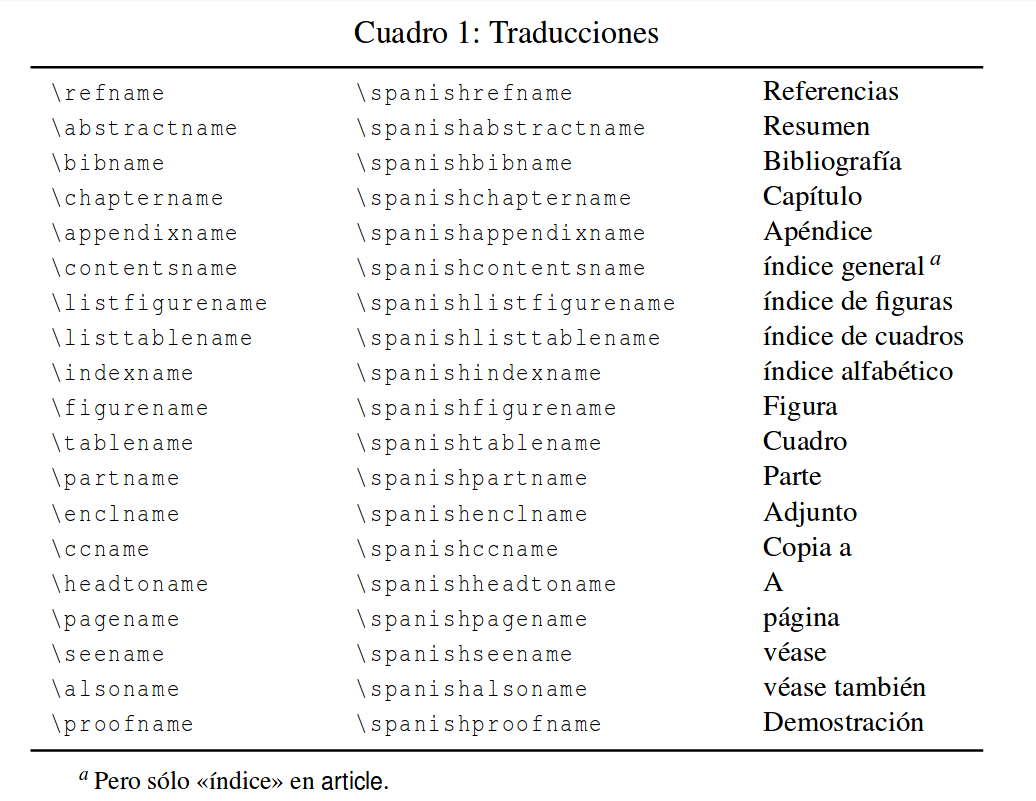
\includegraphics[width=0.9\textwidth]{docs/Figuras/traducciones}
\caption{Tabla que nos dice cómo llama a cada uno de los elementos. Del manual del estilo \lstinline!spanish! del paquete \lstinline!babel!}
\end{figure}

En el caso concreto de las tablas y para \lstinline!pdflatex! podemos cargar el
paquete \lstinline!babel! con la opción \lstinline!es-tabla! y nos evitamos problemas, pero para
el resto de elementos tenemos que hacer lo que os cuento.

\subsubsection{El caso polyglossia}

Si usamos \lstinline!polyglossia!, en su manual dicen que tenemos que cambiar el
nombre de la palabra clave con \lstinline!\gappto! (o \lstinline!\addto! para que sea compatible
con \lstinline!babel!)\footnote{A pesar de que \href{http://tex.stackexchange.com/questions/82993/how-to-change-the-name-of-document-elements-like-figure-contents-bibliogr}{leí} 
(y \href{https://ondahostil.wordpress.com/2017/02/09/lo-que-he-aprendido-establecer-el-idioma-para-xelatex/}{escribí}) que esos nombres se cambiaban
con el comando \texttt{\addto} en el manual de español de \lstinline!babel! dicen que es
mejor usar directamente renewcommand y spanishtablename o el nombre que corresponda.}. Por ejemplo:

\begin{lstlisting}[language={[latex]tex}]
\gappto\captionsspanish{\renewcommand{\tablename}{Tabla}}
\end{lstlisting}

\subsection{Texto en diferentes idiomas}\label{texto-en-diferentes-idiomas}

La última cosa que os voy a contar sobre los paquetes de idioma es cómo
cambiamos de idioma en un mismo documento.

\subsubsection{El caso \texttt{babel}}

En este caso simplemente cargamos como opciones del paquete \lstinline!babel! todos
los idiomas que vamos a usar en el documento:

\begin{lstlisting}[language={[latex]tex}]
\usepackage[idioma1, idioma2]{babel}
\end{lstlisting}

Los vamos activando en el texto con \lstinline!\selectlanguage!:

\begin{lstlisting}[language={[latex]tex}]
\usepackage[spanish, english]{babel}
\selectlanguage{spanish}

\begin{document}

  \section{Sección en español}

  \selectlanguage{english}
  \section{Section in english}

\end{document}
\end{lstlisting}

\subsubsection{El caso \texttt{polyglossia}}

Si estamos usando \lstinline!polyglossia!, cargamos el paquete y establecemos los
idiomas en el preámbulo de la siguiente manera:

\begin{lstlisting}[language={[latex]tex}]
\usepackage{polyglossia}
\setmainlanguage[Opciones]{Idioma} % Idioma principal
\setotherlanguage[Opcions]{Idioma} % Otro idioma
\end{lstlisting}

Si queremos cambiar el idioma de un trocito pequeño de texto usaremos el
comando \lstinline!\textIDIOMA!. Por ejemplo, para poner la fecha en español
haríamos:

\begin{lstlisting}[language={[latex]tex}]
\textspanish{\today}
\end{lstlisting}

Si vamos a escribir un pedazo de texto largo en otro idioma, es
preferible que usemos el entorno correspondiente al idioma;

\begin{lstlisting}[language={[latex]tex}]
\begin{spanish}
  Texto en español
\end{spanish}
\end{lstlisting}

\section{La codificación}\label{sec:codificacion}

La otra parte importante a la hora de configurar el idioma en LaTeX es
la codificación. Hay dos tipos de codificación: la codificación de
entrada y la codificación de fuente.

Configurar la codificación de entrada correctamente para nuestro idioma
nos permite escribir directamente los caracteres especiales desde el
teclado, por ejemplo, poder poner \lstinline!á! en lugar de \lstinline!\'a!.

Una codificación de fuente correcta, por su parte, sirve para que LaTeX
pueda partir las palabras por donde debe y para que podamos buscar en el
pdf resultante palabras con caracteres especiales. Si usamos una
codificación de fuente inadecuada ocurren cosas curiosas como que no
podamos copiar de un pdf palabras que contengan \emph{fi}. Esto se debe a que
LaTeX trata \emph{fi} como un único carácter, ya que es una \href{https://es.wikipedia.org/wiki/Ligadura_(tipograf\%C3\%ADa)}{ligadura
tipográfica}.

Aquí nos ocurre exactamente lo mismo que antes, dependiendo del
compilador tenemos que usar o no diferentes paquetes.

\subsection{El caso de pdflatex}\label{sec:pdflatex}

El pobre \lstinline!pdflatex! es viejecito y necesita ayuda para gestionar la
codificación. Nos hacen falta los siguientes paquetes:

\begin{itemize}
\item
  \lstinline!inputenc!: gestiona la codificación de entrada. Como opción le daremos
  la codificación, para ahorrarnos problemas usaremos \href{https://en.wikipedia.org/wiki/UTF-8}{UTF 8}
\item
  \lstinline!fontenc!: gestiona la codificación de fuente. Para escribir en
  castellano, usaremos la codificación \href{https://en.wikipedia.org/wiki/Cork_encoding}{T1} que contiene los caracteres
  necesarios de los idiomas que usan alfabeto latino con acentos. Si
  queréis escribir en cirílico no os vale esta codificación, tendréis
  que usar la T2A.
\item
  \lstinline!lmodern! o \lstinline!cm-super!: la fuente que LaTeX usa por defecto, Computer
  Modern, no es compatible con la codificación T1 así que necesitaremos
  usar su variante Latin Modern (paquete \lstinline!lmodern!) o la Computer Modern
  Super (paquete \lstinline!cm-super!). Parece ser que la Latin Modern es mejor para
  los acentos y la CM Super para el cirílico.
\end{itemize}

Si queremos escribir en español, la parte del idioma en el preámbulo
para \lstinline!pdflatex! nos queda por lo tanto así:

\begin{lstlisting}[language={[latex]tex}]
\usepackage[spanish]{babel}
\usepackage[utf8]{inputenc} 
\usepackage[T1]{fontenc}
\usepackage{lmodern}
\end{lstlisting}

Para cualquier otro idioma con acentos o caracteres especiales
necesitamos los mismos paquetes y solo tendríamos que cambiar la opción
de idioma en el paquete \lstinline!babel!.

\subsection{Xelatex y otros compiladores
modernos}\label{sec:xelatex}

Los compiladores modernos gestionan ellos solitos la codificación de
entrada y la de fuente así que no es necesario que añadamos ningún
paquete extra. Qué bien ¿eh?

\section{En resumen, ¿qué hago?}\label{sec:resumen6}

Después de todo el rollo que os he soltado, vamos a recapitular y ver
qué necesitamos en cada caso.

Para compilar con \lstinline!pdflatex! añadimos esto al preámbulo:

\begin{lstlisting}[language={[latex]tex}]
\usepackage[spanish,es-tabla]{babel} % Cargamos es-tabla para Tabla en lugar de Cuadro
\usepackage[utf8]{inputenc} % Codificación de entrada
\usepackage[T1]{fontenc} % Codificación de fuente
\usepackage{lmodern} % Fuente compatible
\end{lstlisting}

Para compilar con \lstinline!xelatex! añadimos esto al preámbulo:

\begin{lstlisting}[language={[latex]tex}]
\usepackage{polyglossia}
\setmainlanguage{spanish}
% Para Tabla en lugar de Cuadro
\gappto\captionsspanish{\renewcommand{\tablename}{Tabla}} 
\end{lstlisting}

Podemos venirnos arriba, utilizar el paquete \lstinline!ifxetex! (que mira si
estamos compilando con \lstinline!xelatex!), añadir este trocito al preámbulo y
asegurar que funciona con los dos compiladores:

\begin{lstlisting}[language={[latex]tex}]
% Idioma
\ifxetex
  \usepackage{polyglossia}
  \setmainlanguage{spanish}

  % Tabla en lugar de cuadro
  \gappto\captionsspanish{\renewcommand{\tablename}{Tabla}  
          \renewcommand{\listtablename}{Índice de tablas}}

\else
  \usepackage[spanish,es-tabla]{babel}
  % Para los acentos (xelatex no lo necesita)
  \usepackage[utf8]{inputenc} 
  \usepackage[T1]{fontenc}
  \usepackage{lmodern}
\fi
\end{lstlisting}

Os he añadido la parte de cambiar \emph{Cuadro} por \emph{Tabla} pero, por supuesto,
no es necesario.

\section{Referencias}

\href{http://osl.ugr.es/CTAN/macros/latex/required/babel/base/babel.pdf}{Manual
del paquete \texttt{babel} (pdf)}

\href{http://tug.ctan.org/tex-archive/language/spanish/babel/base/spanish.pdf}{\emph{Estilo
spanish para el sistema babel} (pdf)}

\href{http://osl.ugr.es/CTAN/macros/latex/contrib/polyglossia/polyglossia.pdf}{Manual
del paquete \texttt{polyglossia} (pdf)}

\href{http://mirror.utexas.edu/ctan/macros/latex/doc/encguide.pdf}{\emph{LaTeX
font encodings}}


\chapter{Formas, tamaños y colores}
Con este título tan críptico quería hacer referencia al formato del
texto. Hasta ahora hemos escrito cosas pero nos hemos conformado con el
que nos aparece por defecto, hoy vamos a aprender a cambiar el tamaño y
estilo de la letra y a escribir en diferentes colores. Pero para ello
antes de nada tenemos que entender qué es una clase y cómo afecta a
nuestro documento.

\section{Clases}\label{sec:clases}

Lo primero que tenemos que saber es que el formato de nuestro documento
está definido por su clase. Ahí pondrá cómo de grande tienen que ser los
títulos, cuánto espacio tiene que haber entre los ítems de una lista o
el tamaño de los márgenes. Estas clases pueden ser las típicas
\lstinline!article! o \lstinline!book!, unas que vivan en un paquete
como las \href{http://www.ctan.org/pkg/tufte-latex}{clases Tufte} o
incluso unas que hayamos escrito nosotros mismos. Son simplemente un
archivo \emph{cls} lleno de definiciones.

La clase del documento la establecemos en la definición inicial:

\begin{lstlisting}[language={[latex]tex}]
% Usar la clase memoir
\documentclass{memoir}
\end{lstlisting}

Ahora que sabemos que el estilo de nuestro documento lo decide la clase,
vamos a ver cómo cambiar alguna cosa puntual en el documento. Digo
puntual porque si queremos, por ejemplo, que todos los títulos de
sección sean en cursiva es preferible que redefinamos la orden en
cuestión. Ya haremos eso en el futuro, no os preocupéis.

\section{Formato de texto}\label{sec:formato}

Empecemos modificando el texto. Vamos a cambiar su tamaño, le
aplicaremos diferentes estilos y, por último, haremos una pequeña
introducción al color en LaTeX.

\subsection{Tamaño}\label{sec:tamano}

La manera en la que LaTeX trata el tamaño de letra es bastante original:
coge como referencia el tamaño de la letra del cuerpo del documento y
define los demás tamaños de manera relativa respecto a este. Así, si
cambiamos el tamaño de letra del cuerpo todo lo demás cambia en
consonancia.

Recordemos que el tamaño de letra del cuerpo lo podemos establecer como
argumento opcional en \lstinline!\documentclass!:

\begin{lstlisting}[language={[latex]tex}]
\documentclass[11pt]{article}
\end{lstlisting}

Si no ponemos nada, usará
\href{http://tex.stackexchange.com/questions/155896/what-is-the-default-font-size-of-a-latex-document\#155899}{10pt}
por defecto.

En esta tabla del libro sobre
\href{https://en.wikibooks.org/wiki/LaTeX/Fonts\#Sizing_text}{LaTeX en
Wikibooks} están los comandos para agrandar y reducir la letra y su
respectivos tamaños de letra según el tipo de documento que estemos
creando. Tanto \lstinline!article! como \lstinline!book! son parte de
las
\href{http://tex.loria.fr/ctan-doc/macros/latex/doc/html/usrguide/node10.html}{clases
estándar}.

\begin{figure}[htbp]
\centering
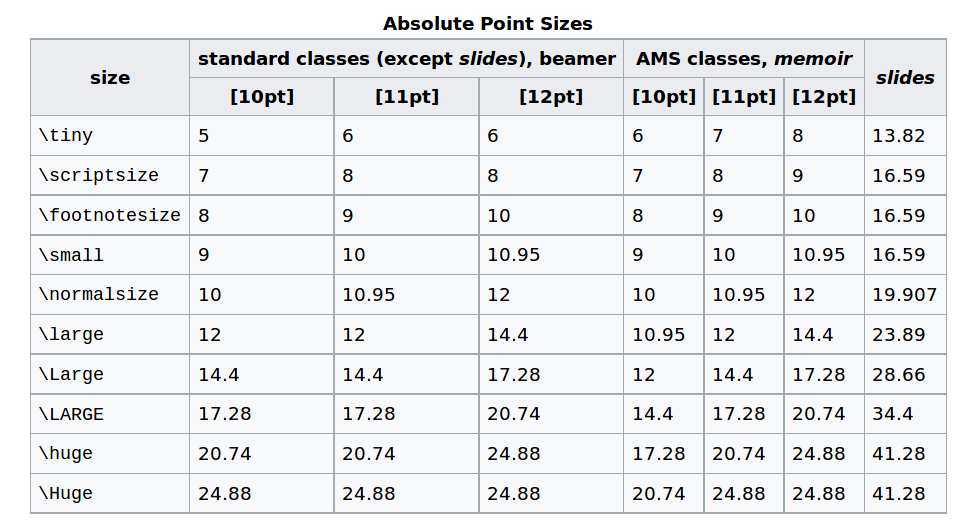
\includegraphics[width=0.9\textwidth]{docs/Figuras/tamanoLetra.png}
\end{figure}

Para usar cualquiera de estos comandos hay dos opciones, usarlos dentro
de una línea o como entorno. Si los usamos en la propia línea, harán
efecto hasta el final del \emph{grupo} (una zona delimitada entre
llaves) o \emph{entorno} actual. Si la zona de aplicación no está
delimitada, el tamaño de letra se mantendrá hasta encontrarse con otro
comando de tamaño o hasta el final del documento. Veamos un ejemplo para
entenderlo mejor:

\begin{lstlisting}[language={[latex]tex}]
Texto normal {\Huge Texto gigantesco}

\normalsize Texto normal hasta nueva orden

\section{\Huge Título de sección enorme}

Texto normal

\begin{quote}
  \Large Letra grande solo para la cita
\end{quote}

Texto normal de nuevo

\small Texto pequeño hasta el final del documento
\end{lstlisting}

Si el trozo de texto que queremos personalizar es muy largo, tal vez
merezca la pena usar el entorno para ganar en legibilidad:

\begin{lstlisting}[language={[latex]tex}]
\begin{tiny}
    Miniletrilla 
\end{tiny}
\end{lstlisting}

También podemos establecer otros tamaños de letra como haríamos en los
editores de toda la vida. Para ello utilizamos el comando
\lstinline!\fontsize!:

\begin{lstlisting}[language={[latex]tex}]
\fontsize{tamaño}{baseline skip}\selectfont Texto
\end{lstlisting}

Podemos facilitar ambos argumentos en diferentes unidades, si no ponemos
más que el número, LaTeX entenderá que estamos hablando de
\emph{puntos}. El segundo argumento es importante, ya que fija la
distancia
\href{http://noodle.med.yale.edu/latex/latex2e-html/baselineskip.html}{\lstinline!\\baselineskip!},
es decir, la distancia entre las partes inferiores de dos líneas
sucesivas. Suele ser 1.2 veces el tamaño de fuente\footnote{He de decir
  también que ponernos a cambiar estas cosas sin dominar es el camino
  directo al infierno del LaTeX en el que todo queda mal y arreglamos
  una cosa y se rompe otra y no sabemos por qué.}.

Si utilizamos este sistema es preferible que usemos una \emph{fuente
vectorial}, así estará disponible en cualquier tamaño\footnote{Para una
  explicación mejor sobre los tipos de fuente podéis echarle un ojo al
  artículo de la
  \href{https://en.wikipedia.org/wiki/Computer_font}{Wikipedia}.}. Por
ejemplo, con Computer Modern es probable que nos salga un aviso de este
estilo:

\begin{lstlisting}[language={[latex]tex}]
LaTeX Font Warning: Font shape `OT1/cmr/m/n' in size <20> not available
(Font)              size <20.74> substituted on input line 25.
\end{lstlisting}

Esto ocurre porque la fuente
\href{https://en.wikipedia.org/wiki/Computer_Modern}{Computer Modern} es
del tipo
\href{https://en.wikipedia.org/wiki/Computer_font\#Bitmap_fonts}{\emph{bitmap}},
es decir, las letras están formadas por puntitos. Esto implica que hay
versiones de la fuente para tamaños concretos, no para todos. En este
caso, lo más fácil es pasarnos a
\href{http://www.gust.org.pl/projects/e-foundry/latin-modern}{Latin
Modern} (\lstinline!\usepackage{lmodern}!) que es igualita y como es
\href{https://es.wikipedia.org/wiki/OpenType}{OpenType} (y por lo tanto
vectorial) no tiene este problema. Además es compatible con la
codificación T1, algo que necesitamos
\href{https://ondahostil.wordpress.com/2017/02/21/curso-no-convencional-de-latex-a-vueltas-con-el-idioma/}{si
vamos a escribir acentos}.

\subsection{Forma}\label{sec:forma}

De momento en el tema de las formas vamos a ignorar el tipo de fuente y
vamos a hablar de negritas, cursivas y esas cosas. Sobre el tipo de
fuente hablaremos en el futuro, que
\href{https://ondahostil.wordpress.com/2016/12/03/lo-que-he-aprendido-escribir-una-carta-en-latex/}{da
para rato}.

Una cosa que aprendí yo hace poquito es que en LaTeX el estilo de cada
letra pertenece a una \emph{familia}, una \emph{serie} y una
\emph{forma}:

\begin{itemize}
\itemsep1pt\parskip0pt\parsep0pt
\item
  La familia indica cómo es la fuente: con serifas o \emph{roman}
  (\lstinline!\rmfamily!), sin serifas (\lstinline!\sffamily!) o
  monoespaciada (\lstinline!\ttfamily!)
\item
  La serie hace referencia al grosor del trazo: fino
  (\lstinline!\lfseries!), medio (\lstinline!\mdseries!) o grueso
  (\lstinline!\bfseries!)
\item
  La formas como su nombre indica describen la forma de las letras:
  recta (\lstinline!\upshape!), cursiva
  (\lstinline!\itshape), oblicua (!\slshape`) o
    versalita (`\scshape`).
\end{itemize}

La letra por defecto tiene serifas, es de grueso medio y recta, es a lo
LaTeX denomina \lstinline!\normalfont!. Podemos hacer otras
combinaciones siempre con un elemento de cada grupo. Saber esto es
especialmente útil cuando estamos definiendo nuestro propio estilo.

Podemos activar diferentes familias, series y formas con diferentes
comandos{[}\^{}comand{]}:

\begin{itemize}
\itemsep1pt\parskip0pt\parsep0pt
\item
  \lstinline!\textbf{}! pone el texto en negrita
\item
  \lstinline!\textit{}! sirve para activar la cursiva
\item
  \lstinline!\texttt{}! escribe en letra de máquina de escribir o
  monoespaciada
\item
  \lstinline!\textsc{}! para las versalitas
\item
  \lstinline!\textnormal{}! vuelve a \lstinline!\normalfont!
\end{itemize}

Hay claramente un patrón, ¿verdad?

Podemos anidar estos comandos y escribir en letra monospaciada, cursiva
y negrita simultáneamente si nos parece que es una buena idea. En
cualquier caso, este es un tema complejo y esto no deja de ser una
explicación un poco por encima, en las referencias podéis encontrar más
información.

Como veis, no aparece la opción de subrayar porque es una
\href{http://practicaltypography.com/underlining.html}{muy mala decisión
tipográfica} que proviene de los tiempos en los que se escribía a
máquina. Si aun así queréis subrayar porque sois tercos como mulas, lo
que estáis buscando es el comando \lstinline!\underline{}!. También
tenéis el paquete \href{http://www.ctan.org/pkg/ulem}{\lstinline!ulem!},
que proporciona el comando \lstinline!\ul! para subrayar y del que me
niego a hablar.

Una cosa interesante es el comando \lstinline!\emph{}! que sirve para
enfatizar. En general se comporta como la cursiva aunque con un par de
pequeñas diferencias:

\begin{itemize}
\itemsep1pt\parskip0pt\parsep0pt
\item
  Depende del contexto, por ejemplo, si enfatizamos un trozo que estaba
  ya en cursiva se pone recto:
\end{itemize}

\begin{lstlisting}[language={[latex]tex}]
\textit{Texto en cursiva \emph{texto recto}}
\emph{Texto en cursiva \emph{texto recto}} 
\end{lstlisting}

\begin{itemize}
\itemsep1pt\parskip0pt\parsep0pt
\item
  Podemos modificarlo para enfatizar a nuestro gusto, ya sea en negrita,
  con colores o lo que sea. Es precisamente lo que hace el paquete
  \lstinline!ulem! (\emph{underline emphasis})
\end{itemize}

\subsection{Color}\label{sec:color}

¡Por fin llegamos al color! Tenía ganas ya, es cansino todo en blanco y
negro. Como suele ser habitual, para usar colores en LaTeX necesitamos
un paquete: \href{http://www.ctan.org/pkg/xcolor}{\lstinline!xcolor!},
la evolución del paquete
\href{https://www.ctan.org/pkg/color}{\lstinline!color!}. Lo cargamos en
el preámbulo con unas pocas opciones que nos facilitan la vida:

\begin{lstlisting}[language={[latex]tex}]
\usepackage[usenames,dvipsnames,svgnames,table]{xcolor}
\end{lstlisting}

\begin{itemize}
\item
  \lstinline!usenames! permite que llamemos a los 16 colores básicos por
  su nombre en lugar de por su definición
\item
  \lstinline!dvipsnames! nos da acceso a otros 64 colores extra
\item
  \lstinline!svgnames! añade otros 150 colores más
\item
  \lstinline!table! nos deja usar colores en las tablas
\end{itemize}

Tenéis una explicación sobre los colores disponibles en el apartado
\href{http://osl.ugr.es/CTAN/macros/latex/contrib/xcolor/xcolor.pdf}{2.4
del manual de \lstinline!xcolor!}.

Para cambiar el color del texto podemos usar tanto
\lstinline!\textcolor! como \lstinline!\color!:

\begin{lstlisting}[language={[latex]tex}]
\textcolor{red}{texto de color rojo}

{\color{magenta} texto en color rosa raro}
\end{lstlisting}

Al igual que ocurría con los comandos para cambiar el tamaño de letra,
en este caso \lstinline!color! afecta hasta el final del grupo.

También podemos definir nuestros propios colores con
\lstinline!\definecolor! dándoles un nombre o directamente cuando los
vayamos a usar. Para ello necesitamos elegir un modelo de color (rgb,
cmyk, HTML, \ldots{}) y darle el valor correspondiente:

\begin{lstlisting}[language={[latex]tex}]
% RGB
\definecolor{azulito}{rgb}{0.36, 0.54, 0.66}

% HTML (en hexadecimal y mayúsculas)
\definecolor{otroColor}{HTML}{4070A0}

% Definir directamente al usarlo
{\color[HTML]{4070A0} texto en color}
\end{lstlisting}

Definir nuestros propios colores es especialmente útil cuando queremos
combinar los colores del texto con alguno específico de una imagen o si
las opciones \lstinline!dvipsnames! y \lstinline!svgnames! no nos
funcionan por algún motivo. En la página
\href{http://latexcolor.com/}{\emph{LaTeX color}} hay montones de
definiciones de colores para que empecemos a jugar.

\section{El resumen}\label{sec:resumen7}

Vamos a hacer una recapitulación sobre lo que hemos visto hoy, que es
largo y denso:

\begin{itemize}
\item
  \textbf{Tamaño}: los tamaños en LaTeX son relativos y se cambian con
  comandos que van de \lstinline!\tiny! para la letra más pequeña a
  \lstinline!\Huge! para la más grande. También se puede establecer un
  tamaño de fuente concreto, pero con cuidado.
\item
  \textbf{Forma}: los estilos de las letras se dividen en familias,
  series y formas que pueden combinarse entre sí. A cada elemento le
  corresponde un comando que activa un formato específico. El texto por
  defecto tiene serifas, es de grueso medio y recto, se conoce como
  \lstinline!\normalfont!.
\item
  \textbf{Color}: para usar colores en LaTeX necesitamos el paquete
  \lstinline!xcolor!. Sus diferentes opciones nos dan acceso a un número
  de colores predefinidos pero también existe la posibilidad de definir
  unos nosotros con \lstinline!\definecolor{modelo}{definición}!.
  Aplicamos al texto cualquiera de estos colores con
  \lstinline!\textcolor{color}{texto}! o con \lstinline!\color{color}!.
\end{itemize}

\section{Referencias}\label{sec:referencias7}

\href{http://texcatalogue.ctan.org/bytopic.html\#classes}{\emph{Classes}
en \emph{The TeX catalogue}}

\href{http://tex.stackexchange.com/questions/782/what-are-the-available-documentclass-types-and-their-uses}{\emph{What
are the available ``documentclass'' types and their uses?} en
StackExchange}

\href{http://www.ctan.org/pkg/tufte-latex}{\emph{Tufte-LaTeX} en CTAN}

\href{https://www.sharelatex.com/learn/Line_breaks_and_blank_spaces}{\emph{Line
breaks and blank spaces}}

\href{http://tex.stackexchange.com/questions/74353/what-commands-are-there-for-horizontal-spacing\#74354}{\emph{What
commands are there for horizontal spacing?} en TexExchange}

\href{https://en.wikibooks.org/wiki/LaTeX/Fonts}{\emph{LaTeX/Fonts} en
Wikibooks}

\href{https://www.sharelatex.com/learn/Font_sizes,_families,_and_styles}{\emph{Font
sizes, families, and styles}}

\href{https://www.tug.org/pracjourn/2006-1/schmidt/schmidt.pdf}{\emph{Font
selection in LaTeX: The most frequently asked questions} (pdf)}

\href{http://www.cl.cam.ac.uk/\%7Erf10/pstex/latexcommands.htm}{\emph{LaTeX
font commands}}

\href{https://github.com/wspr/fontspec}{\emph{The \lstinline!fontspec!
package}}

\href{https://en.wikibooks.org/wiki/LaTeX/Page_Layout\#Margins}{\emph{LaTeX/Page
Layout} en WikiBooks}


\chapter{La página}
En el capítulo anterior estuvimos hablando de los diferentes estilos que
le podemos dar al texto, ahora nos centraremos en el formato de la
propia página. Vamos a ver cómo configurar cuatro cosas que los que
venimos de editores tipo Libre Office echamos de menos: la alineación,
el interlineado, los márgenes y la sangría. Va un
\href{https://www.xkcd.com/378/}{\emph{spoiler}}:

\begin{quote}
There is a LaTeX package for it
\end{quote}

\section{Alineación}\label{sec:alineacion}

Os habréis fijado que LaTeX justifica el texto por defecto, algo que a
mí personalmente me encanta. Para cambiar la alineación tenemos comandos
y entornos equivalentes, los comandos hacen efecto en el grupo actual y
los entornos en su contenido. Tanto los unos como los otros valen tanto
para el texto como para las tablas y figuras:

\begin{itemize}
\itemsep1pt\parskip0pt\parsep0pt
\item
  Para \textbf{alinear a la izquierda} tenemos el entorno
  \lstinline!flushleft! (\emph{nivelado a la izquierda}) y el comando
  \lstinline!\raggedright! (\emph{desigual a la derecha})
\item
  Para \textbf{alinear a la derecha} podemos elegir entre el entorno
  \lstinline!flushright! (\emph{nivelado a la derecha}) y el comando
  \lstinline!\raggedleft! (\emph{desigual a la izquierda})
\item
  Para \textbf{centrar} podemos usar el entorno \lstinline!center! o el
  comando \lstinline!\centering!
\end{itemize}

Hay dos diferencias entre usar un entorno y un comando para alinear:

\begin{itemize}
\item
  El entorno añade espacio blanco adicional delante y detrás de su zona
  de aplicación
\item
  El comando necesita un comando que le diga dónde acaba el párrafo, es
  por ello que se usa dentro de entornos como \lstinline!figure! o
  \lstinline!quote!. En un caso general tendremos que añadir una línea
  en blanco o el comando \lstinline!\par! al final del párrafo.
\end{itemize}

Los comandos son bastante prácticos cuando ya estamos dentro de un
entorno porque nos evitamos escribir otro \lstinline!begin! y
\lstinline!end! y, además, mejoramos la legibilidad.

Van unos ejemplos de texto alineado a la derecha:

\begin{lstlisting}[language={[latex]tex}]

% Texto alineado a la derecha

% Opción 1: entorno flushright
\begin{flushright}
  Texto
\end{flushright}

% Opción 2: \raggedleft + \par
{\raggedleft Texto\par}

% Opción 3: \raggedleft + línea en blanco
{\raggedleft Texto

}

% Opción 4: \raggedleft + entorno que indica final de párrafo
\begin{quote}
  \raggedleft
  Texto
\end{quote}
\end{lstlisting}

Acabo de descubrir que en español se puede uno referir a la alineación
como \href{http://glosariografico.com/bandera}{\emph{bandera}}, es
decir, un texto alineado a la derecha tendrá \emph{bandera a la
derecha}, porque parece una bandera cuyo mástil está a la derecha. Qué
cosas que aprendemos, oiga.

\section{Interlineado}\label{sec:interlineado}

Antes de deciros cómo cambiar el interlineado os dejo con este extracto
del artículo
\href{http://www.tex.ac.uk/FAQ-linespace.html}{\emph{Double-spaced
documents in LaTeX}} de \href{http://www.tex.ac.uk/index.html}{la lista
de preguntas frecuentes de LaTeX\footnote{También os podría contar como
  tuve que escribir mi Proyecto de Investigación en Arial 12, con
  interlineado de 1.5 y unos márgenes que daban ganas de llorar a pesar
  de que estaba usando LaTeX. Todo ello porque había unas
  \emph{exigencias de formato}, algo muy genial teniendo en cuenta que
  ese documento pasaba por un supuesto comité en el que nadie se lo
  leía. \href{http://writer2latex.sourceforge.net/}{Writer2Latex} me
  salvó la vida ahí. Pero mejor lo dejamos para otro día.}}:

\begin{quote}
Of course, the real solution (other than for private copy editing) is
not to use double-spacing at all. Universities, in particular, have no
excuse for specifying double-spacing in submitted dissertations: LaTeX
is a typesetting system, not a typewriter-substitute, and can (properly
used) make single-spaced text even more easily readable than
double-spaced typewritten text.
\end{quote}

Se refiere al interlineado doble, pero lo mismo me vale para cualquiera
que no sea el simple. Pero, como todo en LaTeX, lo podemos cambiar si
nos da por ahí, qué demonios. Para ello según ese mismo documento, lo
mejor es usar el paquete
\href{https://www.ctan.org/pkg/setspace}{\lstinline!setspace!} ya que
mantiene el interlineado simple en los pies de figura y tabla o en las
notas al pie, sitios donde no nos aporta nada que las líneas estén más
separadas.

Simplemente cargamos el paquete y elegimos el interlineado:

\begin{lstlisting}[language={[latex]tex}]
% Preámbulo
\usepackage{setspace}

\doublespacing % Interlineado doble
% \onehalfspacing % Interlineado 1.5
% \singlespacing % Interlineado simple
\end{lstlisting}

\section{Márgenes}\label{sec:margenes}

Para los márgenes, como en los demás casos, lo mejor es usar un paquete
que gestione las cosas por nosotros. Yo uso
\href{http://ctan.org/pkg/geometry}{\lstinline!geometry!} porque es el
que usa Pandoc y yo confío ciegamente en él.

Tan fácil de usar como cargar el paquete dándole como argumento opcional
el tamaño del margen. Para un margen uniforme haríamos:

\begin{lstlisting}[language={[latex]tex}]
\usepackage[margin=1cm]{geometry}
\end{lstlisting}

Y para definir cada margen por su lado:

\begin{lstlisting}
\usepackage[top=1cm, bottom=1cm, right=0.5cm, left=1.5cm]{geometry}
\end{lstlisting}

Para más detalles siempre está disponible
\href{http://osl.ugr.es/CTAN/macros/latex/contrib/geometry/geometry.pdf}{el
manual}

\section{Sangría}\label{sec:sangria}

Las normas tipográficas nos dicen que para separar dos párrafos podemos
usar una
\href{http://practicaltypography.com/first-line-indents.html}{línea en
blanco o sangría},
\href{https://www.youtube.com/watch?v=LbDMJ5YMaxM}{pero no ambas cosas}.
Si no le decimos nada, LaTeX se decanta por la segunda opción. Para
separar los párrafos con líneas en blanco lo más fácil es usar el
paquete \href{http://ctan.org/pkg/parskip}{\lstinline!parskip!}. También
podríamos poner \lstinline!\noindent! delante de cada párrafo que no
queremos que se indente o usar \lstinline!\setlength{\parindent}{0cm}!,
pero el paquete \lstinline!parskip! afecta al documento completo y nos
evita problemas con la gestión del espacio.

Lo cargamos en el preámbulo y a correr:

\begin{lstlisting}[language={[latex]tex}]
\usepackage{parskip}
\end{lstlisting}

\section{Recapitulemos}\label{sec:recapitulemos}

Como recomendación general a la hora de tocar el formato:

\begin{quote}
Lo mejor es dejarle siempre a LaTeX las decisiones de estilo. Él sabe de
tipografía y nosotros no, si hurgamos la probabilidad de convertir el
documento en una cosa que dé dolor de ojos es muy alta.
\end{quote}

Y como recapitulación a lo que hemos visto sobre la página:

\begin{itemize}
\item
  \textbf{Alineación}: LaTeX justifica por defecto pero podemos cambiar
  el alineado con entornos y comandos, \lstinline!flushleft! y
  \lstinline!\raggedright! alinean a la izquierda;
  \lstinline!flushright! y \lstinline!\raggedleft! a la derecha y
  \lstinline!center! y \lstinline!\centering! al centro.
\item
  \textbf{Interlineado}: de por sí es simple y el paquete
  \lstinline!setspace! nos ayuda a cambiarlo mediante órdenes como
  \lstinline!\doublespacing!.
\item
  \textbf{Márgenes}: se pueden modificar con el paquete
  \lstinline!geometry! mandándole los valores de los márgenes al paquete
  como argumento opcional.
\item
  \textbf{Sangría}: LaTeX sangra la primera línea de cada párrafo
  (excepto el primero) pero podemos modificar este comportamiento con el
  paquete \lstinline!parskip!.
\end{itemize}

\section{Referencias}\label{sec:referencias8}

\href{https://en.wikibooks.org/wiki/LaTeX/Page_Layout}{\emph{LaTeX/Page
Layout} en WikiBooks}

\href{http://texblog.org/2011/09/30/quick-note-on-line-spacing/}{\emph{Quick
note on line spacing}}

\href{https://en.wikibooks.org/wiki/LaTeX/Paragraph_Formatting\#Paragraph_indent_and_break}{\emph{Paragraph
indent and break} en WikiBooks}

\href{https://www.phy.duke.edu/~rgb/General/latex/ltx-300.html}{\lstinline!\\raggedleft!
en Hypertext Help with LaTeX}


\chapter{Espacio en blanco}\label{ch:blanco}
\section{Espacio en blanco}\label{espacio-en-blanco}

Como hemos visto en anteriores entregas, LaTeX gestiona el espacio en
blanco él solito. Esto tiene varias implicaciones:

\begin{itemize}
\item
  Le da igual que pongamos un espacio o sesenta y cuatro entre dos
  palabras, para él serán un único espacio.
\item
  Partirá las líneas donde mejor le venga a no ser que nosotros le
  obliguemos a hacerlo en un sitio determinado, dónde hayamos saltado de
  línea en el editor le da absolutamente igual. Lo mismo puede decirse
  de las páginas.
\item
  Dos trozos de texto que no estén separados por una línea en blanco
  pertenecerán al mismo párrafo a no ser que le digamos expresamente que
  no es así.
\item
  No pintará una línea en blanco a no ser que le digamos expresamente
  que lo haga por muchas líneas en blanco que tengamos en el editor.
\end{itemize}

Así visto parece que es malvado y que le gusta fastidiarnos, pero que él
tome las decisiones de formato tiene la grandísima ventaja de que
obtenemos un documento con \emph{pinta profesional} con muy poco
esfuerzo.

En cualquier caso, como nos gusta cacharrear, vamos a ver cómo menear
alegremente las cosas por el documento en contra de la lógica interna de
LaTeX. Aunque en general es mejor y más práctico dejar que LaTeX haga lo
que le dé la real gana. Avisados estáis.

\subsection{Espacio horizontal}\label{espacio-horizontal}

Hay muchas maneras de generar espacio en blanco en LaTeX, demasiadas
para mí. Os voy a hablar de las que yo uso, si queréis convertiros en
expertos en el espacio horizontal tenéis las referencias.

Primero tenemos los dos comandos que ya vimos en el capítulo de
ecuaciones:

\begin{itemize}
\item
  \lstinline!\,! crea un espacio estrecho (\lstinline!\thinspace!). Se
  usa cuando queremos separar ligeramente dos
  \href{http://defharo.com/tipografia/glifos/}{glifos} porque
  interfieren entre sí.
\item
  \lstinline!~! crea un \emph{espacio duro}, es decir, un espacio que no
  se puede partir. Es especialmente útil para las iniciales o casos como
  \emph{Ejemplo 1} donde no queremos que el uno vaya a otra
  línea\footnote{¿Recordáis el comando \lstinline!\refeq!? Lo definimos
    usando un \emph{espacio duro} por este mismo motivo:
    \lstinline!\newcommand{\refeq}[1]{Ecuación~\ref{#1}}!}.
\end{itemize}

Hay muchos más comandos de este tipo cada uno con sus reglas de uso pero
no sé cómo de útil es saberse una pila de ellos sin entender de
tipografía. Solo voy a citar la pareja \lstinline!\quad! y
\lstinline!\qquad! que equivalen respectivamente a 1 em\footnote{Un
  espacio de la anchura de una letra \emph{m} en la fuente actual} y a 2
em porque aparecen a menudo por ahí.

Por otra parte tenemos un comando que nos permite introducir un espacio
blanco del tamaño que nosotros queramos:

\begin{lstlisting}
\hspace{LONGITUD}
\end{lstlisting}

Esta longitud puede estar definida en cualquiera de las medidas que
LaTeX entiende: puntos (\emph{pt}), pulgadas (\emph{in}), centímetros
(\emph{cm}), milímetros (\emph{mm}), \emph{em}, \emph{ex}\footnote{Un
  espacio de la altura de una letra \emph{x} en la fuente actual
  {[}pica{]}: https://en.wikipedia.org/wiki/Pica\_(typography)} o
{[}picas{]}{[}pica{]} (\emph{pc}).

Una cosa a tener en cuenta es que LaTeX ignorará el
\lstinline!\hspace{}! si viene justo después de un salto de línea ya que
para él las líneas no pueden empezar con espacio en blanco. Nos ocurre
exactamente lo mismo al final de las líneas. Podemos obligarle a que
ponga siempre el espacio con la versión con asterisco
\lstinline!\hspace*{}!:

\begin{lstlisting}
% Diferencia entre \hspace y \hspace*
\hspace{1em}Línea alineada

\hspace*{1em}Línea movida 1 em hacia dentro 
\end{lstlisting}

Un comando similar a \lstinline!\hspace{}! es \lstinline!\phantom{}!,
que nos genera un espacio en blanco igual de ancho que su argumento:

\begin{lstlisting}
% Hueco del tamaño de abc
\phantom{abc}
\end{lstlisting}

Finalmente tenemos \lstinline!\hfill!, el \emph{espacio de goma}. Este
comando crea todo el espacio que puede dentro de una línea y sirve para
situar cosas espaciadas pero con un cierto orden en la línea:

\begin{lstlisting}
Texto a la izquierda \hfill Texto a la derecha
\end{lstlisting}

Todos estos comandos de espacio nos vienen bien a la hora de diseñar una
portada para nuestro documento o para crear encabezados y pies de página
personalizados.

\subsection{Espacio vertical}\label{espacio-vertical}

El espacio vertical se gestiona de manera muy similar al horizontal con
los comandos \lstinline!\vspace{}! y \lstinline!\vfill!. El primero nos
permite crear espacio vertical del tamaño deseado. Tiene una versión con
asterisco para que LaTeX no ignore el espacio vertical tras un salto de
página, es decir, al inicio de la página.

El segundo, \lstinline!\vfill!, nos crea \emph{espacio de goma} vertical
y es especialmente útil
\href{http://tex.stackexchange.com/questions/2326/vertically-center-text-on-a-page}{cuando
queremos alinear texto verticalmente}:

\begin{lstlisting}
\vfill
Texto centrado verticalmente
\vfill
\end{lstlisting}

\subsection{Párrafos y saltos de
línea}\label{puxe1rrafos-y-saltos-de-luxednea}

Hemos dicho que para LaTeX un párrafo no acaba hasta que haya una línea
en blanco o alguna indicación extra. Esta indicación es el comando
\lstinline!\par!, que apenas se usa a la hora de escribir ya que empeora
la legibilidad y se suele reservar para definir entornos.

Tenemos que tener en cuenta que solo si estamos usando el paquete
\lstinline!parskip! pintará una línea entre los párrafos, si no, por
mucho que en nuestro editor los párrafos estén separados por una o siete
líneas en blanco veremos dos párrafos juntos con el segundo de ellos
sangrado.

Para provocar saltos de línea tenemos (entre otros menos usados) dos
comandos \lstinline!\\! y \lstinline!\newline!, ambos comienzan una
nueva línea pero no un nuevo párrafo\footnote{Probad a saltar de línea
  sin usar el paquete \lstinline!parskip! ¿la línea tras el salto está
  indentada?}. El primero es preferible dejarlo para alinear, ya que
LaTeX lo redefine según el entorno, por ejemplo en las tablas, para
organizar ecuaciones con \lstinline!align! o tras un
\lstinline!centering!. El segundo solo puede usarse en el texto normal y
a ser posible sin abusar.

\subsection{Saltos de página}\label{saltos-de-puxe1gina}

Lo último que nos queda son los saltos de página. En general uno de
puede despreocupar porque LaTeX tiene la habilidad de situar las cosas
más o menos correctamente en la página. En mi opinión saber saltar de
página es necesario en tres contextos:

\begin{enumerate}
\def\labelenumi{\arabic{enumi}.}
\item
  Queremos una página en blanco al inicio del documento para poner una
  dedicatoria, un resumen, los agradecimientos o algo similar.
\item
  Nos ha empezado una sección muy abajo en la página y no nos gusta cómo
  queda.
\item
  Nos ha almacenado todas las imágenes en una página, la opción H de las
  figuras nos está haciendo cosas raras y tenemos prisa. Meter unos
  saltos de página por ahí nos puede solucionar la papeleta
  momentáneamente.
\end{enumerate}

Vamos a ver las opciones que tenemos:

\begin{itemize}
\item
  \lstinline!\newpage! provoca un salto de página dejando los párrafos
  que quedan tal cual, es decir, con espacio en la parte inferior como
  si se acabase el capítulo.
\item
  \lstinline!\pagebreak! provoca un salto de página y esparce los
  párrafos en la página para no dejar hueco blanco.
\item
  \lstinline!\clearpage! y \lstinline!\cleardoublepage! provocan un
  salto de página y hacen que se pinten todos las figuras y tablas
  definidas hasta ese punto. La diferencia entre ellos es que, como su
  nombre indica, \lstinline!\clearpage! salta una página y
  \lstinline!\cleardoublepage! salta dos caras. Si estamos en un
  documento con diferentes estilos para la página derecha y la izquierda
  \lstinline!\cleardoublepage! saltará las páginas necesarias para que
  la siguiente sea impar.
\end{itemize}

Una vez que hemos identificado los casos posibles y conocemos las
diferentes opciones vamos a combinar las dos cosas para obtener unas
\emph{reglas}:

\begin{itemize}
\item
  Para organizar secciones o figuras podemos elegir entre
  \lstinline!\newpage!, \lstinline!\pagebreak! y \lstinline!\clearpage!
  dependiendo del resultado que queramos conseguir, si es a la mitad de
  un capítulo igual nos conviene más \lstinline!\pagebreak! pero todo es
  probar.
\item
  Para las dedicatorias, resúmenes y tal de los libros la opción
  ganadora es \lstinline!\cleardoublepage! ya que nos los va a poner
  siempre a la derecha como es lo habitual.
\end{itemize}

\section{El resumen}\label{el-resumen}

Os resumo lo que hemos aprendido en este capítulo incluyendo unas
\emph{buenas prácticas}:

\begin{itemize}
\item
  \textbf{Espacio horizontal}: poner un espacio en blanco o varios entre
  dos palabras nos da exactamente el mismo resultado. Hay muchos
  comandos para crear espacio horizontal de mayor o menor tamaño,
  algunos para el texto, otros para las ecuaciones y algunos de ellos
  para ambas cosas. Si queremos crear un espacio a nuestro gusto tenemos
  \lstinline!\hspace{}! y \lstinline!\hspace*{}!, comandos que generan
  un espacio horizontal del tamaño que les pidamos, siendo el del
  asterisco imposible de ignorar. Si queremos un espacio que se ajuste
  solo tenemos \lstinline!\hfill! \emph{que es de goma}.
\item
  \textbf{Espacio vertical}: LaTeX no nos va a crear espacio blanco
  vertical a menos que se lo digamos. Para ello tenemos los comandos
  \lstinline!\vspace{}! y su versión con asterisco que fabrican espacio
  vertical del tamaño que les pidamos. Para situar elementos espaciados
  con cierto equilibrio en la página tenemos el \emph{espacio de goma}
  \lstinline!\vfill!.
\item
  \textbf{Párrafos y saltos de línea}: lo más práctico es separar los
  párrafos con una línea en blanco y solo usar los saltos de línea en
  casos especiales, para ello tenemos \lstinline!\newline! para usar en
  el texto normal y \lstinline!\\! en los entornos especiales.
\item
  \textbf{Saltos de página}: para saltar de página tenemos
  \lstinline!\newpage!, \lstinline!\pagebreak!, \lstinline!\clearpage! y
  \lstinline!\cleardoublepage!. Los tres primeros saltan a la siguiente
  página pero difieren en como tratan el texto y los objetos flotantes
  como las tablas y las figuras. El último salta dos caras y es útil
  para definir la página de dedicatoria o similares de un libro.
\end{itemize}

\section{Referencias}\label{referencias}

\href{https://www.sharelatex.com/learn/Line_breaks_and_blank_spaces}{\emph{Line
breaks and blank spaces}}

\href{http://tex.stackexchange.com/questions/74353/what-commands-are-there-for-horizontal-spacing\#74354}{\emph{What
commands are there for horizontal spacing?} en TexExchange}

\href{https://en.wikipedia.org/wiki/Whitespace_character}{\emph{Whitespace
character} en la Wikipedia}

\href{http://tex.stackexchange.com/questions/82664/when-to-use-par-and-when-or-blank-lines\#82666}{\emph{When
to use \par and when \textbackslash{}, or blank lines} en TexExchange}

\href{http://www.personal.ceu.hu/tex/breaking.htm}{\emph{LaTeX Line and
Page Breaking}}

\href{http://tex.stackexchange.com/questions/736/pagebreak-vs-newpage}{\emph{\lstinline!\pagebreak!
vs \lstinline!\newpage!} en TexExchange}


\chapter{Un documento científico}
Vamos a hablar del caso en el que LaTeX da lo mejor de sí mismo: un
\textbf{documento científico}. Con esto me refiero a libros técnicos,
tesis, artículos\ldots{} ya me entendéis. No tienen por qué hablar
necesariamente de ciencia, si me centro más en ellos es porque es mi
campo.

La característica esencial de un documento científico es su
\emph{formato rígido} que en muchas ocasiones nos viene impuesto, ya sea
por una revista o universidad o por las propias costumbres de nuestra
disciplina. Por ejemplo, una tesis suele estar dividida en capítulos,
debe tener referencias bibliográficas con un estilo determinado y se
inicia con un índice general, uno de tablas y otro de figuras así como
con un glosario de términos. También suele llevar un resumen del
contenido al principio y se separa el trabajo adicional en apéndices.
Todo esto implica diferentes formatos para las partes (numeración de las
páginas y secciones, estilo de los encabezados\ldots{}) y cierta
planificación. Sin planificar se puede uno volver completamente tarumba,
lo digo conocimiento de causa, el control de versiones me salvó más de
una vez de romper la tesis sin remedio.

Es por ello que primero veremos cómo organizar el documento en cuestión
y luego haremos un índice, un glosario y hasta unas lista de
referencias.

\section{División del documento}

Vamos a empezar organizándonos. Lo primero que tenemos que hacer es
elegir el tipo de documento, empezando por preguntarnos si es un
documento corto o largo ya que el formato del documento varía en gran
medida según su longitud:

\begin{itemize}
\item
  \textbf{Documentos cortos}: para ellos usaremos la clase
  \lstinline!article! y sus derivadas, como \lstinline!scrartcl! de las
  \href{https://www.ctan.org/pkg/koma-script}{clases KOMA}. Como norma
  general este tipo de documentos tienen 5 niveles de títulos\footnote{Aprendimos
    a usar los diferentes niveles de título cuando escribimos nuestro
    \href{https://ondiz.github.io/cursoLatex/Contenido/03.DocumentoBasico.html}{primer
    documento}.} (\lstinline!section!, \lstinline!subsection!,
  \lstinline!subsubsection!, \lstinline!paragraph!,
  \lstinline!subparagraph!), con los tres primeros numerados, y no
  llevan portada.
\end{itemize}

\begin{itemize}
\item
  \textbf{Documentos largos}: en este caso nos convienen las clases
  \lstinline!book!, \lstinline!report!\footnote{Estas dos clases sirven
    para objetivos diferentes: \lstinline!report! está pensado para
    documentos no muy largos como un trabajo de clase o así y
    \lstinline!book! para libros verdaderos. Hay varias diferencias
    entre ellas, por ejemplo, la clase \lstinline!book! le da diferentes
    estilos a las páginas pares e impares por defecto mientras que
    \lstinline!report! solo lo hace si se lo pedimos; \lstinline!book!
    abre los capítulos siempre a la derecha aunque pare ello tenga que
    dejar una página en blanco, \lstinline!report! simplemente salta de
    página. Tenéis una comparación mejor
    \href{http://tex.stackexchange.com/questions/36988/ddg\#36989}{aquí}.}
  y sus derivadas como \lstinline!memoir!. Estos suelen tener 7 niveles
  de títulos (\lstinline!part!, \lstinline!chapter!,
  \lstinline!section!, \lstinline!subsection!,
  \lstinline!subsubsection!, \lstinline!paragraph!,
  \lstinline!subparagraph!) de los que se numeran los cuatro primeros.
  Los demás niveles tienen un estilo pero ni se numeran ni aparecen en
  el índice. A diferencia de los documentos cortos, estos llevan portada
  por defecto.
\end{itemize}

Para el caso de un documento largo, si estamos usando las clases
\lstinline!book!, \lstinline!memoir! o derivadas\footnote{\lstinline!report!
  carece de estos comandos el pobrecillo.}, aparte de los diferentes
niveles de títulos tenemos a nuestra disposición unos comandos para
identificar las distintas partes del documento y así darles estilos
específicos. Todos ellos afectan desde que los escribimos hasta que
aparece el siguiente:

\begin{itemize}
\item
  \lstinline!\frontmatter! identifica las páginas preliminares. En esta
  parte los capítulos no llevan número y las páginas se numeran en
  romano. Es donde suelen ir el índice o los agradecimientos.
\item
  \lstinline!\mainmatter! da inicio al cuerpo del documento. Se numeran
  los capítulos y las páginas con números arábigos (o como decían mis
  compañeros de clase \emph{números normales}).
\item
  \lstinline!\appendix! como su nombre indica, especifica dónde empiezan
  los apéndices. Aquí los capítulos se \emph{numeran} con letras pero se
  mantiene numeración de las páginas.
\item
  \lstinline!\backmatter! identifica las páginas finales. En esta parte
  los capítulos no se numeran y, como en los apéndices, se mantiene la
  numeración de las páginas. Nos vale, por ejemplo, para las referencias
  bibliográficas.
\end{itemize}

Por supuesto, todo lo que he comentado sobre los estilos se puede
modificar con relativa facilidad, pero sin tocar absolutamente nada
podemos conseguir un documento con bastante lógica.

Otro tema a tener en cuenta es la \textbf{división del contenido en
diferentes archivos}. Hasta ahora hemos escrito todo junto, pero cuando
estamos escribiendo un documento más o menos largo este sistema no es
muy apropiado. LaTeX nos permite escribir en diferentes archivos que
luego juntaremos para crear el documento final. De esta manera podemos
tener un archivo con la definición del documento y el preámbulo desde el
que llamaremos a otros archivos en los que nos ocuparemos del contenido
propiamente dicho.

Para ello tenemos dos opciones:

\begin{itemize}
\item
  \lstinline!\input{RUTA}! equivale a meter el contenido del archivo ahí
  mismo. Tiene la ventajas de que se puede usar en cualquier parte
  (¡incluido el preámbulo!) y que se puede anidar, es decir, el archivo
  \emph{B} que llamamos desde \emph{A} puede a su vez llamar al archivo
  \emph{C}.
\item
  \lstinline!\include{RUTA}! es un poco más complejo, digamos que nos
  permite \emph{compilar el documento a trozos} porque mantiene los
  números de página, secciones y demás como si compilásemos el documento
  completo aunque solo estemos compilando un pedacito\footnote{Esto
    ocurre porque escribe archivos auxiliares para cada archivo que
    llamamos y luego lee de ahí las referencias, números de página y
    otras cosas que varían. Más adelante hablaremos sobre archivos
    auxiliares, si tenéis ansias podéis leer
    \href{https://ondahostil.wordpress.com/2016/11/17/lo-que-he-aprendido-archivos-auxiliares-de-latex/}{esto
    que escribí hace un tiempo}.}. Es especialmente apropiado para
  capítulos ya que provoca un salto de página antes y después de incluir
  el contenido. Sus desventajas son que no se puede anidar y que no se
  debe usar en el preámbulo.
\end{itemize}

Vamos a ver un ejemplo de uso para entenderlo mejor:

\begin{lstlisting}[language={[latex]tex}]
\documentclass[a4paper,11pt]{book}

  % Cargamos el preámbulo que tenemos escrito en otro archivo
  \input{preámbulo}
  
  % Elegimos qué capítulos queremos que se compilen
  \includeonly{cap1,cap3} % sin espacios!

\begin{document}

  % Cargamos la portada desde la Carpeta contenido
  \input{Contenido/portada}

  % Cargamos los capítulos desde la carpeta Contenido.
  % Los capítulos capX.tex no llevan ni preámbulo ni definición del
  % documento, solo órdenes que irían tras \begin{document}
  
  \include{Contenido/cap1} % cargamos cap1.tex
  \include{Contenido/cap2} % cap2 no aparecerá en el resultado
  \include{Contenido/cap3} % mantiene la numeración como si cap2.tex estuviera incluido

\end{document}
\end{lstlisting}

Ya que tenemos comandos que nos permiten incorporar contenido desde
otros archivos podemos aprovechar para organizar nuestro material en
carpetas para el contenido, el estilo o las imágenes. Incluso cabe la
posibilidad de escribir las tablas largas en un archivo aparte y
llamarlas con \lstinline!\input{}! cuando corresponda. Cuando sepamos
más sobre los diferentes tipos de archivos os contaré cómo me organizo
yo.

\section{Índices}

Pasemos a hablar de los índices, uno de los motivos por los que amo
LaTeX. ¡Los índices de contenido, tablas, figuras o código se hacen
solos! Solamente tenemos que escribir el comando correspondiente y ya
está. La única cosa que tenemos que tener en cuenta es que los índices
no se incluyen por defecto en el índice de contenido, tenemos que
\emph{exigirle} a LaTeX que los añada.

Os pongo un ejemplo de cómo se crean los índices y cómo se incluyen en
el índice, creo que el funcionamiento es bastante claro:

\begin{lstlisting}[language={[latex]tex}]
% Índice de contenido
\addcontentsline{toc}{chapter}{Índice general}
\tableofcontents

% Índice de tablas
\addcontentsline{toc}{chapter}{Índice de tablas}
\listoftables

% Índice de figuras
\addcontentsline{toc}{chapter}{Índice de figuras}
\listoffigures
\end{lstlisting}

Tenemos que tener en cuenta que hay que compilar el documento dos veces
para que LaTeX fabrique los índices, la primera de ellas escribe los
archivos auxiliares necesarios y la segunda los lee y crea el índice en
concordancia.

Como todo en LaTeX, los índices se pueden personalizar. Por ejemplo,
para el caso del índice de contenido, se puede cambiar la profundidad de
los tres niveles que tiene por defecto al número que a nosotros nos
parezca mejor:

\begin{lstlisting}[language={[latex]tex}]
\setcounter{tocdepth}{NIVEL}
% NIVEL -1: part, 0: chapter, 1: section, etc.
\end{lstlisting}

También es interesante darle un título corto para los índices como
argumento opcional a \lstinline!\caption!, \lstinline!\chapter! y otros
comandos, por ejemplo:

\begin{lstlisting}[language={[latex]tex}]
\begin{figure}
  \caption[Título corto para el índice]{Título ultralargo que describe la figura en el documento}
    \includegraphics{RUTA}
\end{figure}
\end{lstlisting}

Para acabar con los índices una cosa bastante chula: si usamos el
paquete \lstinline!hyperref! los elementos de los índices se vuelven
\emph{clicables}. Hasta podemos poner los enlaces de colorines, en mi
tesis, por ejemplo, eran rosas gracias a esta línea:

\begin{lstlisting}[language={[latex]tex}]
\usepackage[colorlinks=true,linkcolor=magenta]{hyperref}
\end{lstlisting}

Dicen en el manual de \lstinline!hyperref! que es mejor que sea el
último paquete que cargamos por si acaso colisiona con algún otro.

\section{Glosario y unidades}

Otro tema que nos interesa a nosotros los científicos es poder hacer una
lista de símbolos, letras griegas o acrónimos con facilidad. Y facilidad
no es coger un documento científico de 350 páginas y apuntar en un
papelito todos los símbolos que hemos utilizado con su respectiva
definición\footnote{Yo me sé de uno que casi gasta el alfabeto griego en
  su tesis y tenía subíndices y superíndices simultáneamente para hacer
  referencia a diferentes variables. Le mando un beso desde aquí.}.

Para el tema de los glosarios, nomenclaturas o listas de
símbolos\footnote{Voy a usar \emph{lista de símbolos} y \emph{glosario}
  indistintamente para referirme a \emph{una lista de cosas con su
  respectiva definición que ponemos al inicio del documento para ayudar
  al lector a entender lo que hemos escrito}} es muy importante la
planificación. \emph{Muy importante}. Lo mejor es configurar todo antes
de empezar a escribir, así aprovechamos las ventajas que tiene usar un
paquete de este estilo y de paso no nos volvemos locos. Por cierto, digo
\emph{un paquete} porque hay unos cuantos con este propósito, aunque
todos ellos tienen dos características en común:

\begin{itemize}
\item
  \textbf{Declaramos los símbolos al principio}. De este modo
  garantizamos la coherencia y no nos llevamos la sorpresa de que le
  hemos llamado \emph{I} a la corriente en el capítulo 3 y \emph{J} en
  el 4. Además, al cambiar la declaración se modifican los símbolos
  correspondientes en todo el documento.
\item
  \textbf{La lista de símbolos se crea automáticamente}. Dependiendo del
  paquete tenemos la opción de crear listas de símbolos, letras griegas
  y acrónimos separadas o no, pero en todos los casos la lista se genera
  automáticamente de manera similar al índice de contenido y solo
  incluye los símbolos que hemos usado en el documento. Esto último
  igual parece ridículo así a primera vista pero nos permite tener
  declarados un montón de símbolos en un archivo aparte y tener la
  certeza de que solo se incluirán los que aparecen en el documento en
  el que estamos trabajando.
\end{itemize}

Veamos qué opciones tenemos. Por una parte están los que usan el
programa
\href{http://tex.loria.fr/bibdex/makeindex.pdf}{\lstinline!makeindex!}
lo que implica un paso extra a la hora de compilar:
\href{http://www.ctan.org/pkg/nomencl}{\lstinline!nomencl!} y
\href{http://www.ctan.org/tex-archive/macros/latex/contrib/glossaries/}{\lstinline!glossaries!},
heredero del antiguo
\href{http://www.ctan.org/pkg/glossary}{\lstinline!glossary!} y que
tiene un manual de 250 páginas. Por otro, tenemos al mucho más modesto
\href{https://www.ctan.org/pkg/listofsymbols}{\lstinline!listofsymbols!}
que tiene menores capacidades pero no nos dificulta la compilación.

Cuando escribí la tesis no tenía ganas de liarme la manta así que me
quedé con \lstinline!listofsymbols! que era sencillito y eficaz. ¡Al
final hasta me atreví a \href{https://gitlab.com/Ondiz/los}{añadirle
funcionalidades} con mis limitadas habilidades! Os dejo un ejemplo de
uso de \lstinline!listofsymbols! que creo que se entiende por sí solo:

\begin{lstlisting}[language={[latex]tex}]
\documentclass{article}

  \usepackage[draft]{listofsymbols} % cambiar 'draft' por 'final' en el definitivo
  \begin{document}

    % Definición de símbolos [Definición]{Nombre que usaremos}[Símbolo]
    \opensymdef
    \newsym[Energía]{symE}{E}
    \newsym[Masa]{symm}{m}
    \newsym[Velocidad de la luz]{symc}{c}
    % Hay que usar \ensuremath en los símbolos matemáticos
    \newsym[Longitud de onda]{symlam}{\ensuremath{\lambda}}
    \closesymdef

    % Crear lista de símbolos
    \listofsymbols

    % Uso en ecuaciones
    \begin{equation}
      \symE=\symm \symc^2
    \end{equation}

    % Uso en texto
    donde \symE es la energía \ldots

\end{document}
\end{lstlisting}

En lo que respecta a \lstinline!nomencl! y a \lstinline!glossaries!,
aunque me parecen interesantes nunca los he usado así que poco más os
puedo decir aparte de este pequeño \emph{estado del arte}. En las
referencias tenéis más información si os animáis a usarlos.

Algo parecido nos pasa con las unidades, por eso voy a hablar de ellas
en este mismo apartado. En este caso se une al tema de la coherencia la
tipografía, una de las mayores preocupaciones de los usuarios de LaTeX
del mundo\footnote{Hay hasta una
  \href{https://nickhigham.wordpress.com/2016/01/28/typesetting-mathematics-according-to-the-iso-standard/}{norma
  ISO} sobre cómo dar formato a las constantes, variables, unidades y
  demás. Y yo he visto a profesores criticar a gente en defensas de
  proyectos \emph{porque no han puesto recto el símbolo de la derivada}.
  Tiene que haber gente para todo.}.

Si nuestro principal problema es que las unidades tengan buena pinta,
tenemos el paquete
\href{http://www.ctan.org/tex-archive/macros/latex/contrib/units/}{\lstinline!units!}
que se ocupa de que nuestras unidades sean tipográficamente correctas.
Gracias a él las unidades tendrán el mismo estilo que el resto del texto
en el modo texto y serán rectas en el modo matemático; no habrá nunca un
salto de línea antes de la unidad, y habrá solo un \emph{espacio
estrecho} (\lstinline!\,!) entre el valor y la unidad. Incluso nos crea
una fracciones de lo más cucas gracias al paquete
\href{http://ctan.org/pkg/nicefrac}{\lstinline!nicefrac!}. Pero la
verdad es que lo uso porque tiene uno de los
\href{http://osl.ugr.es/CTAN/macros/latex/contrib/units/units.pdf}{manuales}
más geniales que he visto yo nunca.

Simplemente lo cargamos en el preámbulo:

\begin{lstlisting}[language={[latex]tex}]
\usepackage{units} % Opción 'ugly' para fracciones de texto normal
\end{lstlisting}

Y usamos los comandos \lstinline!\unit[VALOR]{UNIDAD}! y
\lstinline!\unitfrac[VALOR]{NUM}{DEN}! tanto en el modo texto como
dentro de ecuaciones:

\begin{lstlisting}[language={[latex]tex}]
\unit[3]{m}

$\unitfrac[4]{m}{s}$
\end{lstlisting}

Si aparte de unidades bonitas queremos garantizar la coherencia en todo
el texto tenemos el mucho más potente (y con manual mucho menos
gracioso) paquete
\href{http://ctan.org/pkg/siunitx}{\lstinline!SIunits!}. El enfoque de
\lstinline!SIunits! para las unidades es similar al de los paquetes para
hacer glosarios y al que tiene el propio LaTeX para las ecuaciones: usar
comandos para las unidades en lugar de texto normal. No voy a entrar en
mucho detalle porque es un paquete bastante complejo, pero básicamente
nos da unos comandos para dar formato a números, unidades y números con
unidades:

\begin{lstlisting}[language={[latex]tex}]
% Formato de número
\num[OPCIONES]{NÚMERO}

% Formato de unidad
\si[OPCIONES]{UNIDAD}

% Formato de valor con unidad
\SI[OPCIONES]{VALOR}{UNIDAD}
\end{lstlisting}

Podemos o bien escribir las unidades nosotros mismos o utilizar el
comando correspondiente:

\begin{lstlisting}[language={[latex]tex}]
\si{kg}

\si{\kilogram}
\end{lstlisting}

Es interesante porque nos permite representar las fracciones como
exponentes negativos y los prefijos como \emph{kilo} o \emph{mili} como
potencias de 10:

\begin{lstlisting}[language={[latex]tex}]
\SI{10}{\kilo\metre\per\hour} % 10 km h^{-1}
\SI[per-mode = fraction]{10}{\kilo\metre\per\hour} % 10 km/h
\SI[prefixes-as-symbols=false]{10}{\kilo\metre\per\hour}  % 10 10^3 m h^{-1}
\end{lstlisting}

Todo esto lo podemos configurar en el preámbulo para no tener que
escribir tantísimo, claro. Muchas de las unidades tienen además nombres
cortos para que no sean tan cansinas de definir.

\section{Referencias bibliográficas}

Ahora toca mi parte favorita en lo que respecta a LaTeX y los documentos
científicos: el manejo de las referencias bibliográficas. Para ello
usaremos un programa diferente pero que va integrado en las
distribuciones de LaTeX: el gestor de referencias bibliográficas
\href{http://www.bibtex.org/}{BibTeX}.

BibTeX nos permite tener una base de datos de documentos diversos que
podemos citar en el texto y que luego muy amablemente nos listará donde
le pidamos con nuestro estilo favorito. Lo mejor es que en esa lista
solo aparecerán los elementos que hemos citado y en el orden que
queramos independientemente del orden en el que aparezcan en la base de
datos.

Además, como no era suficientemente genial, tiene dos ventajas extra:
todo va en texto plano y se pueden usar programas libres para generar la
base de datos.

Antes de nada una cosilla, usar BibTeX como yo lo uso es la manera más
sencilla pero también hay otros paquetes más avanzados como
\href{http://ctan.org/pkg/natbib}{\lstinline!natbib!} y
\href{http://ctan.org/pkg/biblatex}{\lstinline!biblatex!} e incluso
otros programas como
\href{http://biblatex-biber.sourceforge.net/}{Biber}, especialmente
desarrollado para trabajar con \lstinline!biblatex!. Aquí me pasa como
con \lstinline!makeindex!, se que existen y poco más. En cualquier caso
os dejo algunos enlaces en las referencias para que os modernicéis, yo
ya no puedo que soy vieja.

Yendo al grano, para mi manera de gestionar la bibliografía necesitamos
lo siguiente:

\begin{itemize}
\item
  \textbf{Una bibliografía}, evidentemente, o bien la tenemos en un
  archivo \lstinline!.bib! o la definimos en el propio documento.
\item
  \textbf{Un estilo de cita} que vendrá definido en un archivo
  \lstinline!.bst!, la propia distribución de
  \href{https://www.sharelatex.com/learn/Bibtex_bibliography_styles}{LaTeX
  trae unos pocos} pero podemos descargarnos uno que nos interese de por
  ahí (por ejemplo, cuando una revista científica nos exige citar de una
  manera determinada) e incluso
  \href{http://ctan.org/pkg/custom-bib}{crear uno nosotros}.
\item
  Si vamos a tener nuestra base de datos en un \lstinline!.bib! nos
  vendrá bien \textbf{programa de gestión bibliográfica}. Puede ser un
  programa específico como los libres
  \href{http://www.jabref.org/}{Jabref} o
  \href{https://www.zotero.org/}{Zotero} o un editor de uso general como
  \href{https://nickhigham.wordpress.com/2016/01/06/managing-bibtex-files-with-emacs/}{Emacs}.
\item
  \textbf{Compilar 4 veces} en una secuencia \lstinline!pdflatex!,
  \lstinline!bibtex!, \lstinline!pdflatex!,
  \lstinline!pdflatex!\footnote{El proceso que se sigue es algo así: el
    primer comando escribe las claves de las referencias en el archivo
    auxiliar. A continuación \lstinline!bibtex! lee esas claves junto
    con el \lstinline!.bib! y el \lstinline!.bst! y crea la bibliografía
    en un archivo \lstinline!.bbl!. El segundo \lstinline!latex! escribe
    las referencias cruzadas en el \lstinline!aux!. Por fin, el último
    escribe las referencias cruzadas en el archivo final.}. He puesto
  \lstinline!pdflatex! pero ya sabemos que puede ser perfectamente
  \lstinline!xelatex! o simplemente \lstinline!latex!. Si estamos usando
  un IDE se hará automáticamente.
\end{itemize}

Vamos a hablar un poco sobre la base de datos bibliográfica. Para mí lo
más simple es usar un programa con su GUI y guardar todo un
\lstinline!.bib!. Este archivo no deja de ser texto plano, de hecho, si
lo abrimos con un editor de texto normal veremos que cada una de las
entradas de nuestra base de datos tiene una pinta como esta:

\begin{lstlisting}[language={[latex]tex}]
@Book{Zarraga2017,
  title={Curso no convencional de LaTeX},
  author={Zarraga, Ondiz},
  year={2017},
  note=\url{https://ondiz.github.io/cursoLatex/}
}
\end{lstlisting}

No voy a hablar sobre ninguno de estos programas aquí por dos motivos:
ya he escrito suficiente tocho y sus manuales están muy bien.

Si no nos gusta usar otro programa, siempre podemos definir la
bibliografía directamente en LaTeX:

\begin{lstlisting}[language={[latex]tex}]
\begin{thebibliography}{9} % Menos de 9 entradas

\bibitem{Zarraga2017}
  Ondiz Zarraga,
  \emph{Curso no convencional de LaTeX},
  2017.

\end{thebibliography}
\end{lstlisting}

En estos dos ejemplos \lstinline!Zarraga2017! es la \emph{clave} de la
entrada bibliográfica y es lo que usaremos para citar ese trabajo en
nuestro documento mediante el comando \lstinline!\cite{CLAVE}!:

\begin{lstlisting}[language={[latex]tex}]
Tal y como dice \cite{Zarraga2017}
\end{lstlisting}

Si hemos escrito nosotros la bibliografía a mano con
\lstinline!thebibliography!, en el documento nos sustituirá
\lstinline!\cite{Zarraga2017}! por un número. Si estamos usando un
archivo \lstinline!.bib!, en cambio, tenemos ventajas añadidas ya que
podemos pedir un estilo de cita y de referencia bibliográfica concreto.
Este estilo está definido en un archivo \lstinline!.bst!, tenéis
explicados los que BibTeX tiene por defecto
\href{https://www.sharelatex.com/learn/Bibtex_bibliography_styles}{aquí}.
En definitiva, necesitamos estas dos líneas:

\begin{lstlisting}[language={[latex]tex}]
% Definimos el estilo bibliográfico
\bibliographystyle{plain} 

% Creamos bibliografía a partir de referencias.bib 
\bibliography{referencias}
\end{lstlisting}

Vamos a dejar aquí la bibliografía, es un tema que da para mucho. Espero
que esto os sirva como introducción, hay más información en las
referencias.

\section{Recapitulación}

Hemos visto que la planificación es fundamental a la hora de escribir un
documento científico. La planificación se extiende tanto a la
organización de los ficheros como a la propia escritura del documento,
ya que elegir una manera de hacer las cosas antes de hacerlas nos ayuda
luego a la hora de trabajar. Por eso yo me haría unas pocas preguntas
antes de escribir la primera letra:

\begin{itemize}
\item
  ¿Qué tipo de documento nos conviene? ¿Hay alguna clase que nos
  facilite la labor?
\item
  ¿Necesitamos crear una lista de símbolos? ¿Vamos a hacerla a mano o es
  preferible usar un paquete? En este último caso, ¿usamos uno
  sencillito o incluimos una etapa extra de compilación para ganar en
  funcionalidad?
\item
  ¿Podría ser interesante un paquete para tratar las unidades? ¿Queremos
  solo que sean bonitas o también cierta coherencia?
\item
  Si nuestro documento tiene referencias bibliográficas ¿cómo vamos a
  crear la base de datos? ¿Qué programa vamos a utilizar?
\end{itemize}

También hemos aprendido que una buena idea para escribir un documento
largo es dividirlo en un archivo en el que se define su esqueleto y
otros en los que está el contenido propiamente dicho. El esqueleto
tendrá una pinta similar a esta:

\begin{lstlisting}[language={[latex]tex}]
% Definición del documento
\documentclass[opciones]{tipo}

% Paquetes
\usepackage[opc]{paquete}

% Datos
\title{título}
\author{autor}
\includeonly{cap1}

% Inicio
\begin{document}
  % Título e índices
  \maketitle

  \frontmatter
  \tableofcontents
  \listoftables
  \listoffigures

  % Contenido
  \mainmatter
  \include{cap1}
  \include{cap2}

  % Apéndices
  \appendix
  \include{ap1}

  % Referencias bibliográficas
  \backmatter
  \bibliographystyle{plain}
  \bibliography{referencias}
  % Fin
\end{document}
\end{lstlisting}

En definitiva, con este fascículo del curso he intentado hablar un poco
de diferentes paquetes y herramientas que tenemos a nuestra disposición
a la hora de escribir un documento científico. Me habré dejado cosas en
el tintero que espero recuperar en el futuro próximo. De momento ahí
están las referencias.

\section{Referencias}\label{referencias}

\href{http://texblog.org/2007/07/09/documentclassbook-report-article-or-letter/}{\emph{\lstinline!\\documentclass\{book, report, 
article or letter\}!} en texblog}

\href{http://tex.stackexchange.com/questions/36988/regarding-the-book-report-and-article-document-classes-what-are-the-mai\#36989}{\emph{Regarding
the \lstinline!book!, \lstinline!report!, and \lstinline!article!
document classes: what are the main differences?} en TexExchange}

\href{http://web.science.mq.edu.au/~rdale/resources/writingnotes/latexstruct.html}{\emph{LaTeX
Notes: Structuring Large Documents}}

\href{http://tex.stackexchange.com/questions/20538/what-is-the-right-order-when-using-frontmatter-tableofcontents-mainmatter\#20547}{\emph{What
is the right order when using \lstinline!\\frontmatter!,
\lstinline!\\tableofcontents!, \lstinline!\\mainmatter!,
\lstinline!\\part!, \lstinline!\\chapter!, \lstinline!\\backmatter!,\lstinline!\\appendix! etc?} en TexExchange}

\href{http://tex.stackexchange.com/questions/246/when-should-i-use-input-vs-include\#250}{\emph{When
should I use \lstinline!\\input! vs. \lstinline!\\include!?} en TexExchange}

\href{http://texblog.org/2011/09/09/10-ways-to-customize-tocloflot/}{\emph{10
ways to customize toc/lof/lot}}

\href{http://get-software.net/macros/latex/contrib/glossaries/glossariesbegin.pdf}{\emph{The
glossaries package v4.25: a guide for beginners} (pdf)}

\href{http://texblog.org/2014/01/15/glossary-and-list-of-acronyms-with-latex/}{\emph{LaTeX
glossary and list of acronyms}}

\href{https://www.sharelatex.com/learn/Nomenclatures}{\emph{Nomenclatures}
en ShareLaTeX}

\href{http://www.math.illinois.edu/~ajh/tex/bibliographies.html}{\emph{LaTeX
tips: Bibliographies}}

\href{https://www.latex-tutorial.com/tutorials/beginners/latex-bibtex/}{\emph{Bibliography
in LaTeX with Bibtex/Biblatex}}

\href{ftp://ftp.dante.de/tex-archive/info/bibtex/tamethebeast/ttb_en.pdf}{\emph{Tame
the BeaST} (pdf)}

\href{https://www.sharelatex.com/learn/Bibliography_management_with_natbib}{\emph{Bibliography
management with \lstinline!natbib!} en ShareLaTeX}

\href{http://tex.stackexchange.com/questions/13509/biblatex-in-a-nutshell-for-beginners}{\emph{\lstinline!biblatex!
in a nutshell (for beginners)} en TeXExchange}

\href{http://www.colorado.edu/physics/phys4610/phys4610_sp13/bibtex_guide.pdf}{\emph{A
BibTeX Guide via Examples} (pdf)}

\href{http://debibify.dorian-depriester.fr/}{\emph{Debibify}, un
colección de estilos de cita}


\chapter{Píntame ese código}
En este episodio vamos a hablar de \emph{resaltado de sintaxis}, es
decir, vamos a aprender a darle formato al código fuente que hayamos
insertado en nuestro documento con la idea de que sea más fácil de leer.

Hay varios paquetes que nos permiten pintar de colorines nuestro código,
está
\href{http://www.ctan.org/tex-archive/macros/latex/contrib/listings/}{\lstinline!listings!}
que he usado bastante,
\href{http://www.ctan.org/tex-archive/macros/latex/contrib/minted/}{\lstinline!minted!}
que tenía ganas de aprender a usar y
\href{http://www.ctan.org/pkg/lgrind}{\lstinline!LGrind!} que descubrí
al escribir esto. Voy a hablar de los dos primeros que son los que
controlo y sobre \lstinline!LGrind! investigáis si os gusta, igual hasta
hay más por ahí.

\section{Lo fácil: listings}

El paquete \lstinline!listings! se utiliza de manera similar al resto de
paquetes que hemos visto hasta ahora: lo cargamos, establecemos sus
opciones y luego utilizamos los comandos que nos proporciona en el
cuerpo del documento.

Para incluir el código hay varias opciones. Por una parte, igual que
ocurría con las ecuaciones y las figuras, podemos escribir código en la
propia línea (\emph{inline}) o puede flotar. Y también como en el caso
de las figuras y ecuaciones, al código flotante podemos ponerle un
\emph{pie de código} (\lstinline!caption!) y etiquetarlo
(\lstinline!label!) para luego referenciarlo en el texto
(\lstinline!\ref{}!).

Para incluir código \emph{inline} tenemos el comando
\lstinline!\lstinline!, muy útil él para hacer referencia a órdenes y
variables en el texto:

\begin{lstlisting}[language={[latex]tex}]
Guardamos el resultado en la variable \lstinline!fib!
\end{lstlisting}

Los signos de exclamación delimitan el código y pueden sustituirse por
cualquier otro carácter no incluido en el código.

Para escribir código con línea propia está el entorno
\lstinline!lstlisting!, al que le podemos dar como opciones tanto el
\emph{pie de código} y su posición como la etiqueta del pedacito de
código:

\begin{lstlisting}[language={[latex]tex}]
% Código con pie en la parte inferior (por defecto en la superior) y etiqueta
\begin{lstlisting}[language=haskell, caption=Código con Listings, captionpos=b, label=lst:fiboHaskell]
  -- Fibonacci!
  fib = 0 : 1 : zipWith (+) fib (tail fib)
\_end{lstlisting}
\end{lstlisting}

Por otra parte, se puede escribir el código en el propio documento o
importarlo de un archivo externo.

\begin{lstlisting}[language={[latex]tex}]
\lstinputlisting[language={[latex]tex}]{Codigo/codigo.tex}
\end{lstlisting}

He puesto precisamente un ejemplo de LaTeX porque tiene una
característica especial: es un \emph{dialecto} de TeX, así veis cuál es
la sintaxis para indicar dialectos.

Este comando es especialmente interesante con los argumentos opcionales
\lstinline!firstline! y \lstinline!lastline! mediante los cuales le
indicamos a LaTeX el trozo de programa que nos interesa pintar:

\begin{lstlisting}[language={[latex]tex}]
\lstinputlisting[language={[latex]tex}, firstline=5, lastline=10]{Codigo/codigo.tex}
\end{lstlisting}

Al igual que con el entorno \lstinline!lstlisting!, al código importado
mediante \lstinline!\lstinputlsiting! podemos ponerle un \emph{pie de
código} con el argumento opcional \lstinline!caption!. Por cierto, si
queremos, podemos recopilar todos los listados de código flotantes en un
índice con el comando \lstinline!\lstlistoflistings!, del mismo modo que
hacíamos con las tablas y las figuras.

Pasemos ahora a personalizarlo. Si no especificamos nada,
\lstinline!listings! nos pintará los comentarios en cursiva, las
palabras claves en negrita y demás, pero todo ello en blanco y negro. Si
queremos otro tipo de formato o usar diferentes colores necesitamos
indicárselo. Veamos cómo se hace.

Lo primero es cargar el paquete \lstinline!xcolor! que, como sabemos de
entregas anteriores nos permite usar colores en nuestro documento:

\begin{lstlisting}[language={[latex]tex}]
\usepackage[usenames,dvipsnames,svgnames,table]{xcolor}
\end{lstlisting}

Luego, en el cuerpo del documento definimos el estilo de nuestro código
con \lstinline!\lstset{OPCIONES}!. Os pongo un ejemplo con diferentes
opciones pero hay muchísimas, lo mejor es mirar en el
\href{http://osl.ugr.es/CTAN/macros/latex/contrib/listings/listings.pdf}{manual}:

\begin{lstlisting}[language={[latex]tex}]
\lstset{
    tabsize=2, % tab = 2 espacios
    backgroundcolor=\color[HTML]{F0F0F0}, % color de fondo
    captionpos=b, % posición de pie de código, b=debajo
    basicstyle=\ttfamily, % estilo de letra general
    columns=fixed, % columnas alineadas
    extendedchars=true, % ASCII extendido
    breaklines=true, % partir líneas
    prebreak = \raisebox{0ex}[0ex][0ex]{\ensuremath{\hookleftarrow}}, % marcar final de línea con flecha
    showtabs=false, % no marcar tabulación
    showspaces=false, % no marcar espacios
    keywordstyle=\bfseries\color[HTML]{007020}, % estilo de palabras clave
    commentstyle=\itshape\color[HTML]{60A0B0}, % estilo de comentarios
    stringstyle=\color[HTML]{4070A0}, % estilo de strings
}
\end{lstlisting}

¿Recordáis que hablamos en su momento de las diferentes familias, series
y formas de las letras? ¿Y de que había dos maneras para aplicarlas?
Aquí se ve clara la utilidad, usamos \lstinline!\bfseries! en lugar de
\lstinline!\textbf! porque \emph{ya estamos dentro de un grupo}.

También tenemos la opción de definir diferentes estilos mediante el
comando \lstinline!\lstdefinestyle{NOMBRE}{ESTILO}! para luego
aplicarlos con la opción \lstinline!style!. A mí en concreto esta
característica me resultó muy útil en la tesis para poder resaltar mejor
el código de Python específico que se usa en Abaqus (¡programa no libre!
¡Huid!), de esta manera tenía un estilo general que se aplicaba a todos
los listados de código y luego unas pocas opciones más que solo se
aplicaban cuando eran necesarias:

\begin{lstlisting}[language={[latex]tex}]
\lstdefinestyle{abaqusPython}{
    language=python,
    % Palabras clave extra
    morekeywords={CONTINUOUS,NUMBER,MESH,par,name,ParStudy,
    template,define,sample,combine, generate},
    % Delimitadores extra, s porque hay uno a cada lado
    moredelim=[s][\ttfamily\color{magenta}]{<}{>},
}

\lstinputlisting[style=abaqusPython]{calculo.py}
\end{lstlisting}

Por último, tenemos que tener en cuenta que \lstinline!listings! no
acepta UTF8 por lo que no nos va a escribir los caracteres acentuados
directamente. Para solucionar esto lo más sencillo es crear un
\lstinline!\lstset! con la opción \lstinline!literate!, que sirve para
sustituir elementos en el código. En sí, \lstinline!literate! se usa
para que el código pueda
\href{https://en.wikipedia.org/wiki/Literate_programming}{leerse con
mayor facilidad}, pero a nosotros nos viene bien para cada vez que vea
\lstinline!á! lo sustituya por \lstinline!\'a! y nos queden bien los
acentos. Os copio aquí lo que yo uso, tenéis una versión con más
chirimbolos
\href{https://en.wikibooks.org/wiki/LaTeX/Source_Code_Listings\#Encoding_issue}{aquí}:

\begin{lstlisting}[language={[latex]tex}]
% Listings no acepta UTF8
{original}{sustitución}{tamaño}
\lstset{literate=
  {á}{{\'a}}1
  {é}{{\'e}}1
  {í}{{\'i}}1
  {ó}{{\'o}}1
  {ú}{{\'u}}1
  {Á}{{\'A}}1
  {É}{{\'E}}1
  {Í}{{\'I}}1
  {Ó}{{\'O}}1
  {Ú}{{\'U}}1
  {ñ}{{\~n}}1
  {ü}{{\"u}}1
  {Ü}{{\"U}}1
}
\end{lstlisting}

La principal debilidad que se le achaca al paquete \lstinline!listings!
es la de no ser un \emph{lexer} completo, es decir, que no distingue
todos los elementos del lenguaje. Para solucionar este problema tenemos
el paquete \lstinline!minted!.

\section{Lo no tan fácil: minted}

El paquete \lstinline!minted! utiliza
\href{http://pygments.org/}{Pygments}, un resaltador de sintaxis general
escrito en Python, para dar formato al código. Está basado además en el
paquete \href{http://www.ctan.org/pkg/fancyvrb}{\lstinline!fancyvrb!}
(\emph{Fancy Verbatim}), un paquete para dar formato al texto
\emph{verbatim}, osease, al \emph{texto tal cual, sin interpretar las
marcas}.

Digo que no es tan fácil porque requiere una etapa de compilación
intermedia y requiere tener Python 2.6 o superior y Pygments instalados.
Para saber si tenemos Pygments instalado podemos buscar el ejecutable
con \lstinline!whereis pygmentize!, que es la
\href{http://pygments.org/docs/cmdline/}{herramienta para el terminal}
de Pygments. Si no lo tenemos siempre nos queda
\lstinline!pip install pygments!.

Que sea un poco más lío de instalar y usar nos da unas ventajas nada
desdeñables:

\begin{itemize}
\item
  Hay disponibles un mayor número de
  \href{http://pygments.org/languages/}{lenguajes}. ¡Hay hasta
  resaltador de
  \href{https://es.wikipedia.org/wiki/Brainfuck}{BrainFuck}!
\item
  Es más fácil de personalizar
\item
  Acepta UTF8, al menos con \lstinline!xelatex! y
  \lstinline!polyglossia!, y hay posibilidad de elegir la codificación a
  partir de su versión 2.0
\item
  Está bien mantenido, hay mejoras del 2016.
\end{itemize}

Evidentemente, también tiene sus desventajas:

\begin{itemize}
\item
  Hay que compilar con la opción
  \href{https://tex.stackexchange.com/questions/20444/what-are-immediate-write18-and-how-does-one-use-them}{\lstinline!-shell-escape!}
  para que LaTeX permita la ejecución de un programa externo, lo que
  implica ciertos \href{https://0day.work/hacking-with-latex/}{problemas
  de seguridad}.
\item
  La versión\footnote{Podemos ver la versión del paquete que estamos
    usando en el archivo \emph{.log}} de los repositorios suele ser
  antigua, con lo que nos perdemos las últimas funcionalidades como la
  de elegir la codificación. Además, es un poco de lío actualizarlo
  porque requiere
  \href{https://www.ctan.org/pkg/fvextra}{\lstinline!fvextra!} y en
  algunos repos no está.
\end{itemize}

Vayamos a su uso. La opción más básica es usar el entorno
\lstinline!minted! junto con el lenguaje del código en cuestión:

\begin{lstlisting}[language={[latex]tex}]
\begin{minted}{python}
 for n in range(10):
   if n%2:
     print n
\end{minted}
\end{lstlisting}

Que tiene la versión reducida \lstinline!\mint! si el código que
queremos añadir tiene solo una línea. Para delimitar el código podemos
usar diferentes caracteres, los elegimos según los delimitadores que use
nuestro código.

\begin{lstlisting}[language={[latex]tex}]
\mint{python}|print [n for n in range(10) if n%2]|
\end{lstlisting}

Tanto para el caso del entorno \lstinline!minted! como para el comando
\lstinline!\mint! el código tendrá línea propia, pero no se le puede
considerar flotante, para ello debemos rodear cualquiera de las dos
opciones con el entorno \lstinline!listing!, más abajo hay un ejemplo
completo en el que se muestra cómo hacerlo.

Este paquete también nos permite incluir código \emph{inline}:

\begin{lstlisting}[language={[latex]tex}]
Guardamos el resultado en la variable \mintinline{python}{fib}
\end{lstlisting}

Y también tenemos la opción de importar el código tal y como hacíamos
con \lstinline!listings!:

\begin{lstlisting}[language={[latex]tex}]
\inputminted{python}{fibonacci.py}
\end{lstlisting}

Lo más difícil de usar de \lstinline!minted! es llamar al comando que
compilará en documento con la opción \lstinline!-shell-escape!, por
ejemplo:

\begin{lstlisting}[language=bash]
pdflatex -shell-escape documento.tex
\end{lstlisting}

Los que compiláis a pelo o con un Makefile no tenéis problema, los que
estáis usando un editor específico para LaTeX seguramente podréis crear
un comando personalizado para compilar. En Kile, que es el programa que
yo uso ahora mismo, tendríamos que ir a \emph{Settings \textgreater{}
Configure Kile \textgreater{} Tools \textgreater{} Build} y crear una
nueva herramienta de compilación que incluya \lstinline!-shell-escape!
siguiendo el ejemplo del resto de herramientas. Digo una \emph{nueva}
porque no es demasiado recomendable compilar alegremente cualquier
documento con la opción \lstinline!-shell-escape! ya que con TeX se
puede programar \emph{cualquier cosa}, hasta cosas malignas.

Para personalizar el código tenemos diferentes opciones:

\begin{itemize}
\item
  Con \lstinline!\usemintedstyle[LENGUAJE]{ESTILO}! elegimos el
  \href{https://help.farbox.com/pygments.html}{estilo de Pygments} con
  el queremos dar formato al código. Como veis el lenguaje es opcional,
  podemos elegir un estilo para cada lenguaje si nos apetece. Para ver
  los estilos instalados escribimos \lstinline!pygmentize -L styles! en
  el terminal. También podemos definir nuestro propio estilo siguiendo
  las \href{http://pygments.org/docs/styles/}{directrices de Pygments}.
\item
  Los comandos \lstinline!\setminted[LENGUAJE]{ESTILO}! y
  \lstinline!\setmintedinline[LENGUAJE]{ESTILO}!, que tiene precedencia,
  también valen para definir los estilos. El primero afecta al entorno
  \lstinline!minted! y al comando \lstinline!\mint! y el segundo al
  código \emph{inline}.
\item
  El comando \lstinline!\newminted[NOMBRE]{LENGUAJE}{OPCIONES}! nos
  permite guardar las opciones para un determinado lenguaje para el
  entorno \lstinline!minted!. Es similar a \lstinline!\lstdefinestyle!
  del paquete \lstinline!listings!. Si no le ponemos nombre llamará
  \lstinline!LENGcode! a nuestro nuevo estilo donde \lstinline!LENG! es
  el lenguaje del mismo. Para usarlo no tenemos más que sustituir el
  nombre del lenguaje por el del estilo que hemos definido en el entorno
  \lstinline!minted!.
\item
  El comando \lstinline!\newmint[NOMBRE]{LENGUAJE}{OPCIONES}! es el
  equivalente a \lstinline!\newminted! para el comando
  \lstinline!\mint!. Funciona exactamente igual excepto por que
  sustituye \lstinline!\mint! por el nombre que le hemos dado al estilo.
\end{itemize}

\begin{lstlisting}[language={[latex]tex}]
\newmint[py]{python}{bgcolor=black}

\py|print [n for n in range(10) if n%2]|
\end{lstlisting}

En cuanto a las opciones, hay montones de ellas, muchas coinciden con
las de \lstinline!listings!, creo que lo mejor es ir al
\href{http://osl.ugr.es/CTAN/macros/latex/contrib/minted/minted.pdf}{manual}
y mirar, se entiende bastante bien y no es demasiado largo.

¡Veamos un ejemplo completo! Tiene las siguientes características:

\begin{itemize}
\item
  Es un objeto flotante con opción de posición H (\emph{here})
\item
  Crea un índice de codigo con \lstinline!\listoflistings!, el
  equivalente a \lstinline!\lstlistoflistings!
\item
  Activa los números de línea con la opción \lstinline!linenos!
\item
  Nos deja escribir ecuaciones en los comentarios del código gracias a
  \lstinline!mathescape!
\item
  Nos permite escribir en LaTeX dentro de los comentarios del código
  gracias a \lstinline!texcl!. Esta opción se ha convertido en
  \lstinline!texcomments! a partir de la versión 2.0. En este caso lo
  uso para poder enlazar la página web.
\end{itemize}

\begin{lstlisting}[language={[latex]tex}]
% Cambiamos Listing por Listado
\renewcommand{\listingscaption}{Listado}
\listoflistings

\begin{listing}[H]
  \begin{minted}[linenos,mathescape,texcl]{clojure}
  ;; Fibonacci por cortesía de \href{https://pfctelepathy.wordpress.com/}{Ekaitz}
  ;; $F_n = F_{n-1} + F_{n-2} \,/\, F_0 = 0 \wedge F_1 = 1$
  (defn fibo
      ([] (fibo 0 1))
      ([one two]
          (lazy-seq (cons one (fibo two (+ one two))))))
  \end{minted}
  \label{lst:fibo}
  \caption{Código con Minted}
\end{listing}
\end{lstlisting}

Que quedaría así:

\begin{figure}[htbp]
\centering
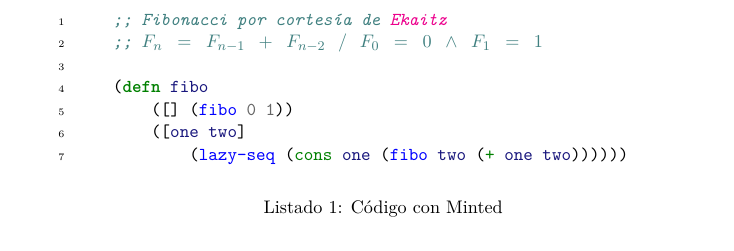
\includegraphics[width=\textwidth]{docs/Figuras/fibo.png}
\caption{Ejemplo de uso de minted}
\end{figure}

Como nota final, \lstinline!listings! no sabe resaltar Clojure y nos
obligaría a crear
\href{http://alexott.net/common/clojure/clj-latex.txt}{nuestro propio
\emph{resaltador}}.

\section{En resumen}\label{en-resumen}

En esta entrega hemos aprendido a resaltar código de dos maneras, una de
ellas usa un paquete de la forma tradicional y la otra llama a un
programa externo. Ambas nos dan una funcionalidad similar siendo tal vez
\lstinline!listings! más fácil de usar y \lstinline!minted! más fácil de
personalizar. Los dos paquetes tienen montones de opciones pero como ya
estamos curtidos, !podemos ir a sus respectivos manuales y leerlos para
saber sacar el máximo partido!

\section{Referencias}\label{referencias}

\href{http://www.texdoc.net/texmf-dist/doc/latex/listings/listings.pdf}{Manual
de \lstinline!listings!}

\href{https://github.com/gpoore/minted}{\lstinline!minted! en GitHub}

\href{http://osl.ugr.es/CTAN/macros/latex/contrib/minted/minted.pdf}{Manual
de \lstinline!minted!}

\href{http://www.tex.ac.uk/FAQ-codelist.html}{\emph{Code listings in
LaTeX} en el FAQ de LaTeX}

\href{https://www.sharelatex.com/learn/Code_listing}{\emph{Code listing}
en ShareLaTeX}

\href{https://tex.stackexchange.com/questions/102596/minted-vs-texments-vs-verbments\#103471}{\lstinline!minted!
vs \lstinline!textments! vs \lstinline!verbments! en TeXExchange}

\href{https://www2.cs.uic.edu/~s/papers/tex2010/}{\emph{Are Text-Only
Data Formats Safe? Or, Use This LaTeX Class File to Pwn Your Computer}}


\chapter{También podemos presentar}
Como muchos ya sabréis, con LaTeX además de fabricar documentos con una
excelente calidad también podemos crear presentaciones. Para ello
tenemos varias clases diferentes,
\href{https://www.ctan.org/pkg/beamer}{\lstinline!beamer!} es la más
famosa y probablemente habréis oído hablar de ella, pero también tienen
el mismo objetivo
\href{http://www.ctan.org/pkg/powerdot/}{\lstinline!powerdot!} y las más
viejecillas \href{http://www.ctan.org/pkg/prosper}{\lstinline!prosper!},
\href{https://www.ctan.org/pkg/seminar}{\lstinline!seminar!} y
\href{http://www.ctan.org/pkg/slides}{\lstinline!slides!}. Yo voy a
hablar de la clase \lstinline!beamer! que es la que controlo, pero antes
de nada vamos a ver en qué nos beneficia usar LaTeX para hacer una
presentación.

\section{¿Merece la pena usar LaTeX para una
presentación?}

He de reconocer que odio Power Point, Impress y todo el software similar
y que la primera vez que usé LaTeX para una presentación fue única y
exclusivamente por llevar la contraria, pero no volvería atrás. Estas
son las ventajas que le veo:

\begin{itemize}
\item
  \textbf{Contenido y formato separados}: esta es una de las
  características fundamentales de LaTeX y aquí nos resulta
  especialmente útil, definimos ambas cosas por separado y se afectan
  muy poco entre sí.
\item
  \textbf{Orden lógico}: nos vemos obligados a escribir el contenido
  como si fuera un texto y no como unos cuadrados con cosas dentro.
\item
  \textbf{Formato favorable para el espectador}: es más complicado poner
  muchísimo texto o imágenes sin ton si son en una diapositiva que
  hacerla sencilla y clara.
\item
  \textbf{Texto plano}: como siempre, trabajamos con texto plano por lo
  que no necesitamos un programa específico\footnote{Luego veremos que a
    la hora de presentar tal vez necesitemos un programa si queremos
    usar alguna funcionalidad específica.}, el resultado no depende del
  sistema operativo\footnote{Algo que importante cuando eres
    \emph{linuxera} en entorno Windows y no quieres que te echen la
    bronca porque \emph{sus} formatos privativos no funcionan en tu
    sistema operativo libre o viceversa, porque tus formatos estándar no
    funcionen en \emph{su} sistema privativo.}, la colaboración más
  sencilla y demás ventajas habituales del texto plano que ya conocemos.
\item
  \textbf{Reutilización}: si la presentación deriva de otro documento,
  como un artículo o tesis, que hemos escrito en LaTeX podemos copiar el
  trozo correspondiente a las imágenes, ecuaciones, tablas\ldots{}
  directamente en la presentación.
\end{itemize}

También tiene, evidentemente, sus inconvenientes:

\begin{itemize}
\item
  \textbf{No vemos lo que hacemos}: esto nos lleva pasando mucho tiempo
  pero puede ser un problema para una presentación ya que es algo más
  visual. Este problema es especialmente acuciante si no tenemos claro
  el orden en el que queremos decir las cosas.
\item
  \textbf{Diseños complejos}: es bastante difícil crear una diapositiva
  con muchos elementos y que siga teniendo buena pinta. Esto quiere
  decir que nunca conseguiríamos reproducir las míticas presentaciones
  comerciales que tienen en cada página el logo de la empresa y su
  slogan, un índice de contenidos, diecisiete imágenes, dos tablas y
  texto en tres tipos de fuente diferen te. A LaTeX le va más el
  minimalismo\footnote{Por cierto, me encanta cuando dicen que con LaTeX
    se crean presentaciones \emph{de calidad} y el ejemplo tiene unos
    colores que hacen sangrar los ojos. Aberraciones estéticas se pueden
    cometer por mucho que usemos LaTeX.}.
\end{itemize}

\section{La clase beamer}

Bien, pasemos entonces a hablar sobre \lstinline!beamer!. Aunque esta
clase tenga un
\href{http://osl.ugr.es/CTAN/macros/latex/contrib/beamer/doc/beameruserguide.pdf}{manual
de casi 250 páginas} enseguida puede uno montarse una presentación
decente. Esto se debe a que las tablas, imágenes,
bibliografía, apéndices\footnote{Para tener apéndices numerados
  necesitamos cargar el paquete \lstinline!appendixnumberbeamer!},
ecuaciones y demás características de LaTeX funcionan exactamente igual,
aunque su aspecto varía dependiendo del estilo que estemos utilizando.
Del mismo modo, \lstinline!\maketitle! nos hace la portada y
\lstinline!\tableofcontents! nos fabrica el índice de contenidos como
viene siendo habitual.

En definitiva, creamos el documento de la misma manera que creábamos un
artículo o libro, definiendo el contenido de cada diapositiva dentro del
entorno \lstinline!frame!:

\begin{lstlisting}[language={[latex]tex}]
\begin{frame}{Título}
  % Contenido de la diapositiva
\end{frame}
\end{lstlisting}

Algo a tener en cuenta es que tanto las secciones como las subsecciones
añaden una entrada al índice pero no establecen el título de la
diapositiva, debemos hacerlo nosotros a mano. Dependiendo del estilo,
tener diferentes secciones y subsecciones nos permite crear diapositivas
de título para separar cada sección y que nuestra presentación pueda
seguirse más fácilmente.

\subsection{Estilo}

En cuanto al estilo debemos diferenciar dos cosas: los \textbf{temas} y
el \textbf{estilo de ciertos elementos} como las alertas, los ejemplos o
los teoremas, que cada tema redefine.

El \textbf{tema} es lo que establece el formato general de nuestra
presentación, vendría a ser como la plantilla. Aparte de los temas que
define el propio \lstinline!beamer! y de los que hablaremos a
continuación, tenemos muchos temas disponibles en Internet, por ejemplo,
en
\href{https://www.overleaf.com/latex/templates/tagged/presentation}{Overleaf}.
A mí me gustan especialmente
\href{https://www.overleaf.com/9480607mxqxvhczzvhr\#/34336424/}{\emph{Presento}},
\href{https://www.overleaf.com/9480660qtjkqtjfqhny\#/34336601/}{el de la
universidad de Berkeley} y
\href{https://www.ctan.org/pkg/beamertheme-metropolis}{Metropolis}, el
que usé con algunas modificaciones para la defensa de mi tesis.

Lo más importante que hay que entender respecto a los temas de
\lstinline!beamer! es que hay cinco tipos:

\begin{itemize}
\item
  \textbf{Temas de presentación}: afectan a toda la presentación. Eligen
  un tema de color, uno de fuente, uno exterior y otro interior que
  combinen (relativamente) bien. Tienen nombres de ciudades.
  Antiguamente se llamaban cosas tipo \lstinline!bars! o
  \lstinline!shadow!.
\item
  \textbf{Temas de color}: afectan a la paleta de colores de la
  presentación. Hay temas de color \emph{exterior}, con nombres de
  animales acuáticos; \emph{interior}, con nombres de flores; y
  completos con nombre de animales voladores. Los temas interiores
  afectan al color de lo de dentro de la diapositiva; los exteriores a
  los elementos del borde y los completos a ambas cosas.
\item
  \textbf{Temas de fuente}: controlan el tipo de fuente que usamos en la
  presentación, por defecto es Sans Serif, pero hay opción de Serif
  (\lstinline!serif!); títulos en negrita (\lstinline!structurebold!),
  títulos en cursiva (\lstinline!structureitalicserif!) y títulos en
  versalita (\lstinline!structuresmallcapsserif!).
\item
  \textbf{Temas interiores}: controlan el aspecto de los elementos del
  interior de la diapositiva, es decir, como se muestran los bloques,
  las tablas, las figuras, las listas\ldots{} Las opciones son
  \lstinline!default!, \lstinline!circles!, \lstinline!rectangles!,
  \lstinline!rounded! e \lstinline!inmargin!. Lo más fácil es probar uno
  mismo que hace cada una, si no se hace muy largo de explicar.
\item
  \textbf{Temas exteriores}: controlan el aspecto de los bordes, es
  decir, el encabezamiento, el pie y la barra lateral. Las opciones son
  \lstinline!default!, \lstinline!miniframe!, \lstinline!sidebar!,
  \lstinline!split!, \lstinline!shadow!, \lstinline!tree! y
  \lstinline!smoothtree!. Podéis probar a ver cuál os gusta más.
\end{itemize}

Podemos combinarlos como nos parezca más bonito. Existen, de hecho,
\href{https://hartwork.org/beamer-theme-matrix/}{matrices} recopilando
combinaciones de estilos, sobre todo para los temas de presentación y de
color.

Para terminar con los temas veamos como se establecen todos ellos:

\begin{lstlisting}[language={[latex]tex}]
% Preámbulo
\usetheme{Bergen} % tema de presentación
\usecolortheme{rose} % tema de color
\usefonttheme{serif} % tema de fuente
\useinnertheme{circles} % tema interior
\useoutertheme{split} % tema exterior
\end{lstlisting}

En el caso de que haya la posibilidad de definir más opciones las
añadimos entre corchetes como argumento opcional, eso ya depende de cada
tema.

En cuanto al \textbf{estilo de los diferentes elementos} de la
presentación, son los temas los que establecen cómo son todos y cada uno
de ellos, por lo que si no nos gusta, por ejemplo, la pinta que tienen
las listas podemos pisar su estilo por defecto el nuestro. Esto nos
permite que nuestra presentación sea coherente y que no tengamos en la
diapositiva 7 el título verde y en la 23 rosa. En el siguiente apartado
veremos cómo se modifica el estilo de los elementos.

\subsection{Opciones}

Lo que sí cambia respecto a otros documentos de LaTeX es el modo de
establecer las opciones, ya que para ello usamos la familia de comandos
\lstinline!\setbeamer! y especificamos qué elemento queremos cambiar y
cómo. Según qué queramos conseguir tenemos diferentes comandos:

\begin{itemize}
\item
  \lstinline!\setbeameroption{opción general}!, establece las opciones
  generales para la presentación. Por ejemplo y tal y como veremos en la
  próxima sección, se usa para decirle a \lstinline!beamer! que muestre
  u oculte las notas mediante \lstinline!\setbeameroption{hide notes}!.
\item
  \lstinline!\setbeamertemplate{elemento}{definición}!, define el
  aspecto de cierto elemento, por ejemplo, con
  \lstinline!\setbeamertemplate{itemize   item}{$\Rightarrow$}!
  conseguimos que en las listas no numeradas se indiquen los ítems con
  una flecha.
\item
  \lstinline!\setbeamercolor{elemento}{fg=colorPrimerPlano, bg=colorDeFondo}!,
  establece el color de determinado elemento, por ejemplo,
  \lstinline!\setbeamercolor{title}{fg=magenta, bg=white}! establece que
  todos los títulos sean rosas con el fondo blanco. No es necesario usar
  las opciones \lstinline!fg! y \lstinline!bg! a la vez, lo que no
  cambiemos mantendrá el color que tenía.
\item
  \lstinline!\setbeamerfont{elemento}{size=tamaño, shape=estilo}!,
  establece la forma y tamaño de fuente de determinado elemento, por
  ejemplo, \lstinline!\setbeamerfont{title}{series=\bfseries}! pone en
  negrita el título de la presentación. Podemos establecer solo el
  tamaño o solo el estilo, lo que no cambiemos permanecerá como estaba.
\end{itemize}

Para ver qué elementos tiene una presentación no nos queda otra que
acudir al
\href{http://osl.ugr.es/CTAN/macros/latex/contrib/beamer/doc/beameruserguide.pdf}{manual},
pero ahora ya sabemos mucho y lo podemos entender perfectamente. También
en el manual encontraremos los argumentos opcionales de estos comandos.

Podemos usar todos estos comandos en cualquier parte del documento y
afectan desde donde están situados hasta encontrarse con otra definición
o, si no hay ninguna más, hasta el final.

\subsection{Notas}

Con \lstinline!beamer! tenemos la opción de crear unas notas secretas
que solo vemos nosotros en la línea de la
\href{https://wiki.openoffice.org/wiki/Presenter_Screen}{consola del
presentador} de Impress. Para escribir las notas usamos el comando
\lstinline!\note{}! que nos crea una página de notas detrás de la
diapositiva en cuestión:

\begin{lstlisting}[language={[latex]tex}]
\documentclass[notes=show]{beamer}
\begin{document}
  \begin{frame}
    % Contenido de la diapositiva
    \note{Notas}
  \end{frame}
\end{document}
\end{lstlisting}

Esto es interesante, pero se le puede sacar mucho más jugo uniéndolo al
paquete \href{http://ctan.org/pkg/pgf}{\lstinline!pgfpages!} que nos
permite unir la diapositiva con la página de notas en una hoja más ancha
de tal manera que al proyectarla nosotros veamos las notas y la
audiencia la presentación. Hay que tener en cuenta que esta
funcionalidad no es compatible con todos los visores de \emph{pdf}, en
el siguiente apartado hablaremos de ello.

Controlamos el comportamiento de las notas mediante las siguiente
opciones:

\begin{itemize}
\item
  \lstinline!\setbeameroption{hide notes}! solo muestra la presentación.
\item
  \lstinline!\setbeameroption{show only notes}! solo muestras las notas.
\item
  \lstinline!\setbeameroption{show notes on second screen=right}! crea
  una presentación el doble de ancha que contiene las diapositivas y las
  notas. En este caso mostramos las notas en la pantalla de la derecha,
  con \lstinline!left! las pondríamos en la izquierda.
\end{itemize}

Veamos como quedaría:

\begin{lstlisting}[language={[latex]tex}]
\documentclass{beamer}

\usepackage{pgfpages}
\setbeameroption{show notes on second screen=right}

\begin{document}
  \begin{frame}
    % Contenido de la diapositiva
    \note{Notas}
  \end{frame}
\end{document}
\end{lstlisting}

\subsection{Efectos y multimedia}

Que hagamos la presentación con \lstinline!beamer! no significa que vaya
a ser aburrida y estática, podemos personalizar cómo va apareciendo el
contenido e incluso añadir multimedia. Os cuento ahora unas cosillas al
respecto.

\paragraph{Overlay}

Mediante las opciones de \emph{overlay} se puede controlar cuando se
muestra cada elemento. Esto nos viene bien, por ejemplo, para mostrar
los elementos de una lista uno a uno. Para ello LaTeX nos creará
múltiples copias de la diapositiva con \emph{overlays} que mostrarán los
elementos que vayamos indicando. De esta manera, al ir avanzando dará la
sensación de que va \emph{surgiendo} o \emph{desapareciendo} contenido
en la presentación.

Hay varios comandos para gestionar este mecanismo, como los que siguen:

\begin{itemize}
\item
  \lstinline!\pause!: solo se muestra el contenido hasta este punto.
\item
  \lstinline!\uncover<OVERLAY>{CONTENIDO}!: solo se muestra el contenido
  en las copias indicadas pero se le reserva espacio desde el principio.
\item
  \lstinline!\only<OVERLAY>{CONTENIDO}!: como \lstinline!\uncover! pero
  sin que se reserve espacio previamente para el contenido.
\end{itemize}

Además, muchos otros comandos y entornos aceptan opciones de
\emph{overlay}, generalmente con esta estructura:

\begin{lstlisting}[language={[latex]tex}]
\comando<OVERLAY>{CONTENIDO}

\begin{entorno}<OVERLAY>
CONTENIDO
\end{entorno}
\end{lstlisting}

En \lstinline!OVERLAY! especificamos cuándo queremos que aparezcan las
cosas, \lstinline!<1>! mostrará el contenido solo en la primera copia;
\lstinline!<2->! en todas a partir de la segunda y \lstinline!<-5>! solo
hasta la quinta.

Un caso interesante es el de las listas, ya que hay una sintaxis
simplificada para mostrar los elementos de uno en uno:

\begin{lstlisting}[language={[latex]tex}]
\begin{itemize}[<+->]
 \item Ítem 1
 \item Ítem 2
\end{itemize}
\end{lstlisting}

Aprovecho el ejemplo para decir que los \emph{overlays} también
funcionan en las notas:

\begin{lstlisting}[language={[latex]tex}]
\note<1>{Notas para el ítem 1}
\note<2>{Notas para el ítem 2}
\end{lstlisting}

\paragraph{Vídeos}
En las presentaciones de \lstinline!beamer! también podemos añadir
vídeos, faltaría más. Hay varios paquetes con este fin, como
\lstinline!multimedia!, que viene con el propio \lstinline!beamer! y
\href{https://www.ctan.org/pkg/media9}{\lstinline!media9!}, que
sustituye a
\href{https://www.ctan.org/pkg/movie15}{\lstinline!media15!}. El
problema aquí es que muy pocos visores de \emph{pdf} soportan los vídeos
incrustados. Si conseguís encontrar uno, los vídeos se incrustan muy
fácilmente:

\begin{lstlisting}
% Vídeo con multimedia
\movie[OPCIONES]{SUSTITUTO}{VÍDEO}

% Vídeo con media9
\includemedia[OPCIONES]{SUSTITUTO}{VÍDEO}
\end{lstlisting}

Donde \lstinline!SUSTITUTO! es el texto o imagen que guardará sitio al
vídeo, por ejemplo, un fotograma del mismo. En \lstinline!VÍDEO! debemos
escribir la ruta al vídeo.

Otra opción es usar el comando \lstinline!\href! del paquete
\href{https://www.ctan.org/pkg/hyperref?lang=en}{\lstinline!hyperref!},
que sirve para crear enlaces en nuestros documentos. En lugar de
incrustar el vídeo en la presentación, en este caso ponemos un texto o
imagen para que cuando la pinchemos se abra el reproductor de vídeo en
una ventana aparte:

\begin{lstlisting}
\href{run:VIDEO}{SUSTITUTO}
\end{lstlisting}

\paragraph{Navegación}

En la parte inferior de las diapositivas nos aparecen por defecto unos
iconitos para navegar por la presentación y buscar. Hay gente que los
ama y gente que los detesta. Si sois de los segundos podéis asesinarlos
con:

\begin{lstlisting}[language={[latex]tex}]
\setbeamertemplate{navigation symbols}{}
\end{lstlisting}

\paragraph{Repetición}

La última cosa que os voy a contar sobre \lstinline!beamer! es cómo
insertar automáticamente un contenido concreto cuando se dé cierto
evento. Esto es útil para hacer aparecer una diapositiva con el título o
para mostrar el índice cada vez que vaya a comenzar una nueva sección,
por poner un par de ejemplo.

Conseguimos esto con la familia de comandos\lstinline!\AtBegin! (y
\lstinline!\AtEnd! para el caso de las notas) que se disparan al
comenzar una sección, parte, nota o demás. Os dejo aquí dos casos que
creo que se entienden con facilidad:

\begin{lstlisting}[language={[latex]tex}]
% Diapositiva con el título de sección al iniciar sección
\AtBeginSection{
  \begin{frame}
  \vfill
  % Caja con colores de título
  \begin{beamercolorbox}[center]{title}
    \usebeamerfont{title} % Fuente de título
    \insertsectionhead % Nombre de sección
  \end{beamercolorbox}
  \vfill
  \end{frame}
}

% Índice mostrando subsección actual al iniciar subsección
\AtBeginSubsection
{   \begin{frame}{Outline}
        \tableofcontents[currentsection,
        currentsubsection,
        sectionstyle=show/hide,
        subsectionstyle=show/shaded/hide] 
    \end{frame}
}
\end{lstlisting}

\section{Programas para presentar}

El mayor problema de \lstinline!beamer! desde mi punto de vista es que
no todos los visores de \emph{pdf} son capaces de mostrarnos en nuestro
ordenador las notas y proyectar las diapositivas. Si somos valientes y
damos las presentaciones a pelo esto no nos importa, con cualquier
lector en pantalla completa estamos servidos, pero si somos cobardicas
con miedo escénico como la que escribe tenemos un problema.

¡No nos asustemos aún! El mundo es grande y los cobardes que usan LaTeX
y saben programar parece que abundan. Es por ello que hay diferentes
alternativas para que podamos hacer trampa y leer de nuestras notas
secretas. En concreto voy a hablar de \emph{pdfpc} que es el que yo he
usado, luego nombraré algunos otros que sé que existen pero poco más.

\subsection{Pdfpc}

\href{https://pdfpc.github.io/}{\emph{Pdfpc}} es una herramienta de
línea de comandos para visualizar presentaciones en formato \emph{pdf}
en varias pantallas. Es un \emph{fork} de \emph{Pdf Presenter Console},
que \href{https://github.com/jakobwesthoff/Pdf-Presenter-Console}{dejó
de desarrollarse}. Se distribuye con licencia
\href{https://github.com/pdfpc/pdfpc/blob/master/LICENSE.txt}{GNU GPL
v2} así que es software libre. Es muy fácil de utilizar y ayuda mucho a
la hora de presentar, no solo por las notas, como luego veremos.

La única pega que le pondría es que tuve que compilarlo desde fuente
porque el que estaba en los repositorios era muy viejecito, pero no es
difícil, yo lo hice en GNU/Linux y hasta en Windows con Cygwin\footnote{Hablé
  un poco más en detalle sobre cómo compilar
  \href{https://ondahostil.wordpress.com/2016/10/24/lo-que-he-aprendido-compilar-pdf-presenter-console-con-cygwin/}{aquí}}.

Para usarlo simplemente escribimos:

\begin{lstlisting}[language={[latex]tex}]
pdfpc PRESENTACIÓN
\end{lstlisting}

Donde \lstinline!PRESENTACIÓN! es la ruta a la presentación en
\emph{pdf}.

De por sí \emph{pdfpc} nos enseña en la vista de presentador la
diapositiva actual, la siguiente, un reloj, el número de la diapositiva
actual y el total. Todo ello muy útil a la hora de presentar.

\begin{figure}[htbp]
\centering
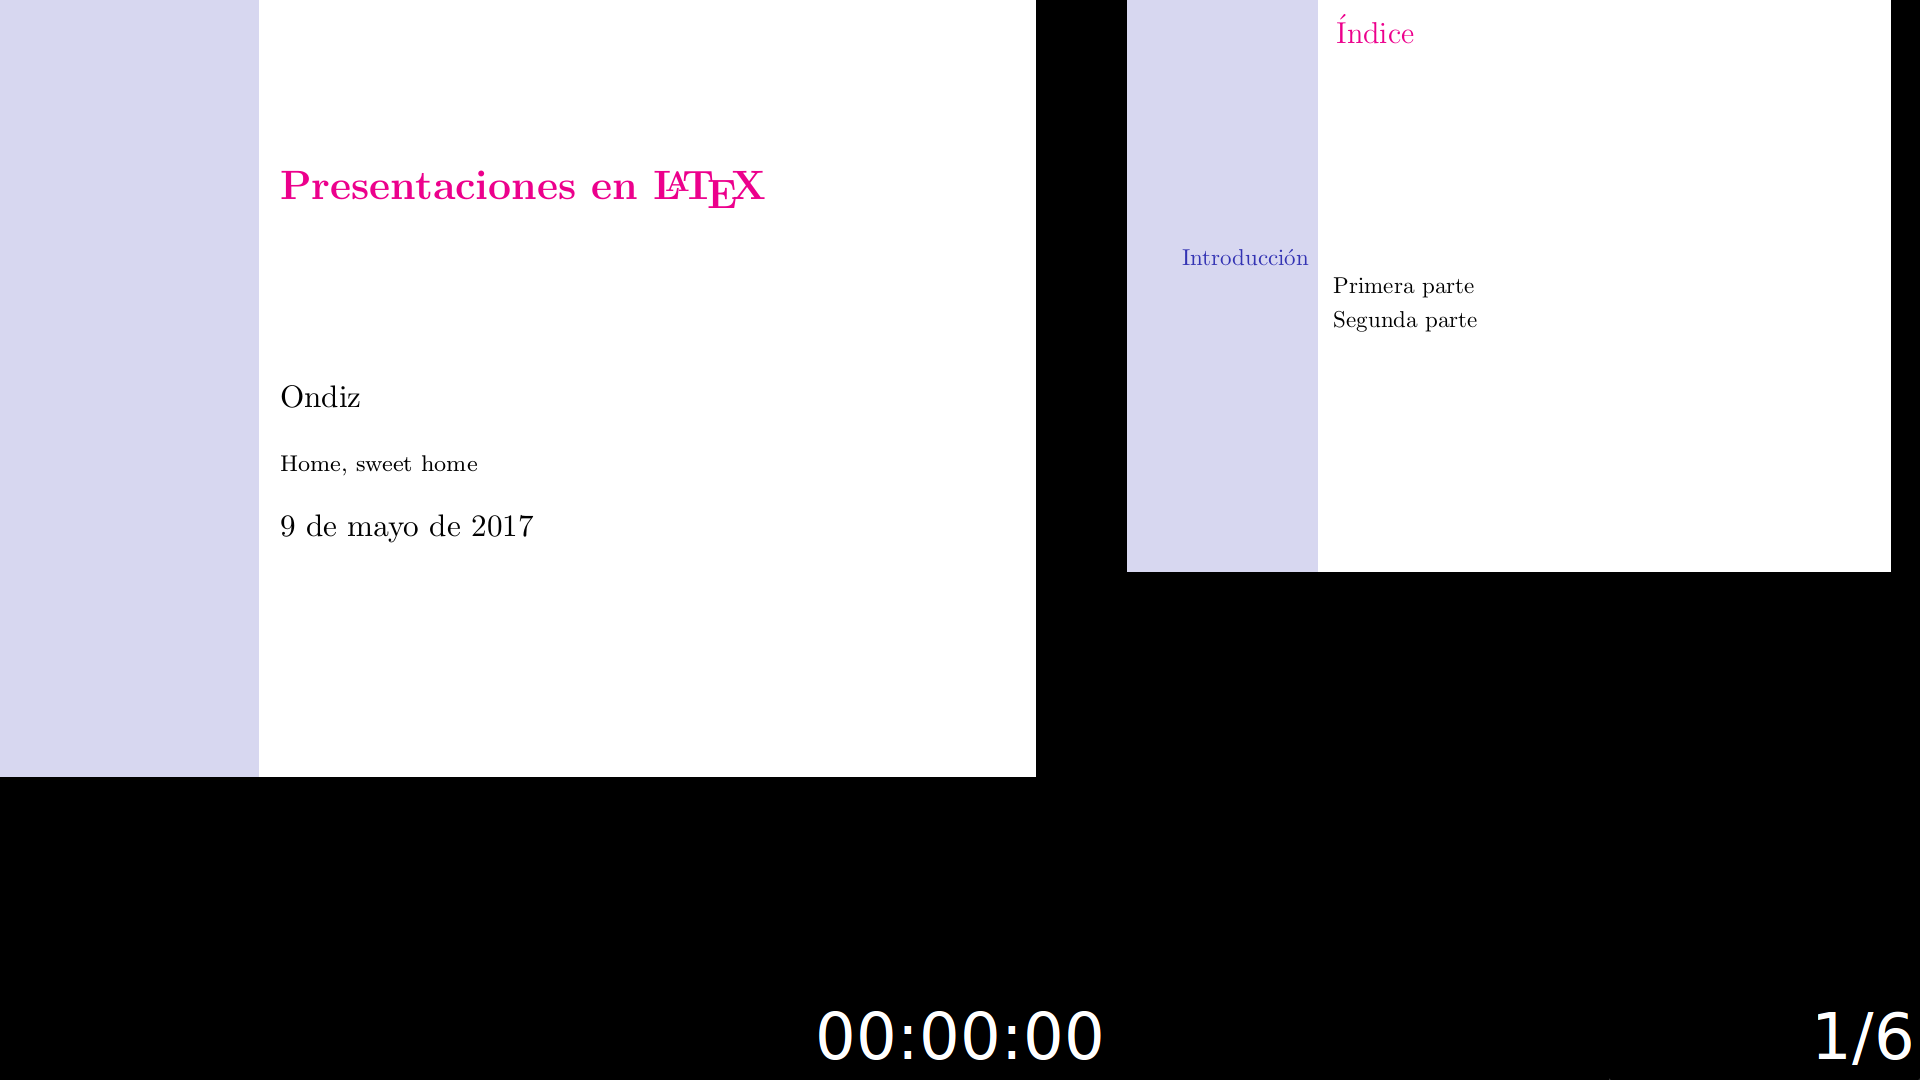
\includegraphics[width=\textwidth]{docs/Figuras/pdfpc.png}
\caption{pdfpc en acción}
\end{figure}

Para ver las notas de \lstinline!beamer! necesitamos crear la
presentación con las notas integradas como hemos visto antes:

\begin{lstlisting}
\setbeameroption{show notes on second screen=right}
\end{lstlisting}

Luego llamamos a \emph{pdfpc} con la opción \lstinline!--notes!:

\begin{lstlisting}[language=bash]
pdfpc presentation.pdf --notes=right
\end{lstlisting}

Ahora en la vista de presentador veremos las notas y una minidiapositiva
mostrándonos la diapositiva actual, en lugar de verla en grande como
antes.

\begin{figure}[htbp]
\centering
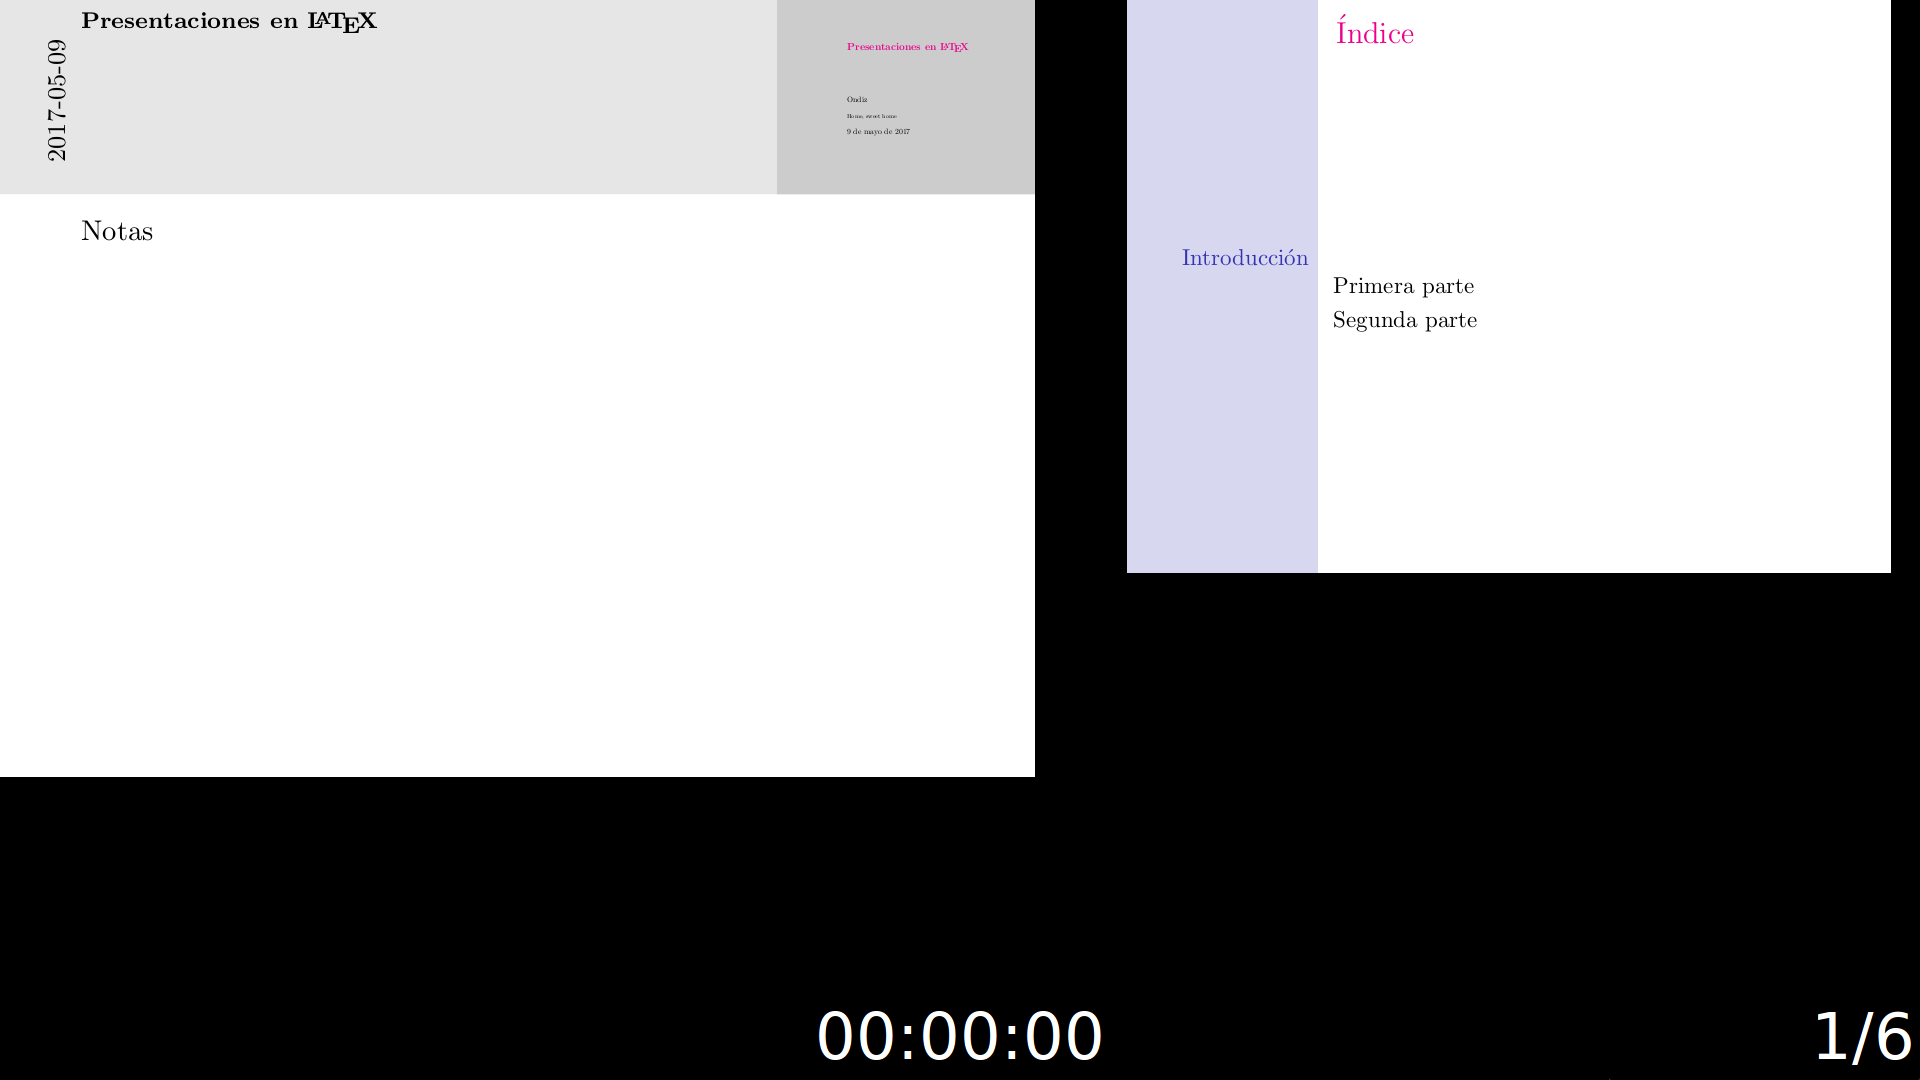
\includegraphics[width=\textwidth]{docs/Figuras/pdfpcNotas.png}
\caption{pdfpc con notas}
\end{figure}

El programa tiene otras muchas opciones, os resumo unas pocas que me
parecen especialmente útiles, las demás están en el manual:

\begin{itemize}
\item
  \lstinline!-d!, \lstinline!--duration=N! la duración en minutos
  (\lstinline!N!) de la presentación. Sirve para que nos ponga una
  cuenta atrás en la parte inferior de la pantalla.
\item
  \lstinline!-l!, \lstinline!--last−minutes=N! tiempo en minutos
  (\lstinline!N!) a partir del que la cuenta atrás se verá en rojo. Para
  irse poniendo nerviosillo.
\item
  \lstinline!-s!, \lstinline!--switch−screens! cambia la vista de
  presentador de pantalla.
\item
  \lstinline!-w!, \lstinline!--windowed! crea dos ventanas, una con la
  vista del presentador y otra con lo que verá la audiencia. Útil para
  ver el resultado cuando solo tenemos una pantalla.
\end{itemize}

Por ejemplo, para presentación de la tesis usé lo siguiente\footnote{Y
  no llegué a la cuenta atrás en rojo porque en media hora lo tenía
  ventilado.}:

\begin{lstlisting}[language=bash]
pdfpc presentation.pdf --duration=45 --notes=right --last-minutes=10
\end{lstlisting}

Además, durante la presentación se pueden usar diferentes teclas para
\emph{hacer cosas}:

\begin{itemize}
\item
  \lstinline!F! (\emph{freeze}): congela la imagen de la presentación
  para la audiencia mientras nosotros jugamos en nuestra vista. Pinta un
  copo de nieve en la parte inferior.
\item
  \lstinline!B! (\emph{black}): pone la pantalla de la audiencia negra y
  a nosotros nos pinta un cuadradito negro con una cruz blanca. Útil
  cuando das clase y alternas pizarra y proyector (así no montas el lío
  que solían montar mis profesores, ingenieros industriales casi todos
  ellos).
\item
  \lstinline!G! (\emph{go}): nos lleva a la diapositiva que le
  indiquemos. Fantástico para cuando te dicen \emph{en la diapositiva 12
  hay una tabla que\ldots{}}
\item
  \lstinline!N! (\emph{notes}): nos permite escribir notas en la
  diapositiva. Salimos con \lstinline!ESC!.
\item
  \lstinline!E! (\emph{end}): marca la diapositiva final. Útil si
  tenemos \emph{diapositivas de repuesto} para las preguntas.
\item
  \lstinline!O! (\emph{overlay}): sirve para marcar/desmarcar
  diapositivas como parte de una diapositiva que va surgiendo poco a
  poco. No las tendrá en cuenta en el cómputo total de diapositivas.
\item
  \lstinline!P! (\emph{pause}): pausa el reloj.
\item
  \lstinline!R! (\emph{reset}): reinicia la presentación.
\item
  \lstinline!Q! (\emph{quit}) o \lstinline!ESC!: cierra la presentación.
\end{itemize}

Las notas y diferentes marcas (fin, \emph{overlay}, \ldots{}) las guarda
en un archivo \emph{pdfpc} que recupera cada vez que leemos la
presentación. Es un archivo de texto plano y podemos abrirlo. Tiene esta
pinta:

\begin{lstlisting}
[file]
presentation.pdf
[duration]
45
[skip]
8,
[end_user_slide]
10
[notes]
### 1
Notas en la diapositiva 1
\end{lstlisting}

\subsection{Otras opciones para
presentar}

Los programas que cito ahora nunca los he usado, encontré \emph{pdfpc} y
me quedé con él, los pongo aquí para que vosotros elijáis el que más os
guste.

\begin{itemize}
\item
  \href{http://impressive.sourceforge.net/}{\emph{Impressive}}\footnote{¡Gracias
    a \href{https://quitter.se/notice/9129937}{Shevek} por informarme de
    su existencia!}: un programa escrito en Python con funcionalidades
  curiosas como el modo foco y la vista global de todas las
  diapositivas.
\item
  \href{https://github.com/Cimbali/pympress}{\emph{Pympress}}: también
  escrito en Python, soporta vídeo y las notas de \lstinline!beamer! y
  tiene una consola para el presentador.
\item
  \href{https://github.com/dannyedel/dspdfviewer}{\emph{Dspdfviewer}}:
  un visor simple para las presentaciones de \lstinline!beamer!.
\end{itemize}

\section{Resumen}

Para resumir lo que hemos estado comentando, vamos a ver cómo quedaría
un ejemplo completo aunque sencillo de una presentación en LaTeX:

\begin{lstlisting}[language={[latex]tex}]
% Definición
\documentclass{beamer}

% Notas
\usepackage{pgfpages}
\setbeameroption{show notes on second screen=right}

% Datos
\title{Presentaciones en \LaTeX}
\author{Ondiz}
\institute{Home, sweet home}
\date{\today}

% Temas
\usetheme{Bergen}
\usefonttheme{serif}
\usecolortheme{rose}

% Opciones
\setbeamercolor{title}{fg=magenta, bg=white}
\setbeamertemplate{navigation symbols}{}

% Inicio
\begin{document}

% Diapositivas
 \begin{frame}
  \maketitle
  \note{Notas}
 \end{frame}
 
 \begin{frame}{Índice}
  \tableofcontents
  \note{Más notas}
 \end{frame}
 
 \section{Introducción}
 \subsection{Primera parte}

 \begin{frame}{Introducción}
  \begin{itemize}
   \item<1-> Ítem 1
   \item<2> Ítem 2
  \end{itemize}
 \end{frame}

\end{document}
\end{lstlisting}

¡No es tan difícil!

En cualquier caso, para empezar con \lstinline!beamer! yo recomendaría
coger una presentación ya hecha y probar a cambiar cosas hasta que nos
sintamos cómodos con este nuevo sistema de trabajo. Cuando ya manejemos
lo más sencillo ir al manual (o a StackOverflow) y personalizar la
presentación es coser y cantar.

Por último, como soy maja os dejo una presentación de
\href{https://github.com/Ondiz/cursoLatex/tree/master/Ejemplos/Presentacion}{ejemplo}
en el repositorio del curso, contiene muchas de las cosas que he
comentado.

\section{Referencias}

\href{https://tex.stackexchange.com/questions/16204/which-package-to-use-for-presentations-beamer-prosper-or-other}{\emph{Which
package to use for presentations? Beamer, Prosper, or Other} en
TeXExchange}

\href{http://www.dmi.me.uk/blog/2010/11/08/creating-a-presentation-with-latex-and-powerdot/}{\emph{Creating
a presentation with LaTeX and powerdot}}

\href{http://osl.ugr.es/CTAN/macros/latex/contrib/beamer/doc/beameruserguide.pdf}{Manual
de \lstinline!beamer!}

\href{https://tug.org/pracjourn/2005-2/miller/miller.pdf}{\emph{Producing
beautiful slides with LaTeX}}

\href{https://hartwork.org/beamer-theme-matrix/}{\emph{Beamer theme
matrix}}

\href{http://www.deic.uab.es/~iblanes/beamer_gallery/index.html}{\emph{Beamer
theme gallery}}

\href{https://www.r-bloggers.com/create-your-own-beamer-template/}{\emph{Create
your own beamer template}}

\href{https://tex.stackexchange.com/questions/1574/embedding-videos-and-animations}{\emph{Embedding
videos and animations} en TeXExchange}

\href{https://tex.stackexchange.com/questions/21777/is-there-a-nice-solution-to-get-a-presenter-mode-for-latex-presentations}{\emph{Is
there a nice solution to get a ``presenter mode'' for Latex
presentations?} en TeXExchange}


\chapter{Nuestras propias macros}
Hoy vamos a salir de mi zona de confort y hablar sobre la creación de
\href{http://foldoc.org/macro}{\emph{macros}}, es decir, de nuevos
comandos y entornos\footnote{¡Líos de nomenclatura a la vista! Dijimos
  hace mucho que LaTeX es un \emph{conjunto de macros} para TeX. Luego
  hemos separado estas \emph{macros} en comandos y entornos, pero un
  entorno no deja de ser un conjunto de comandos que afecta de forma
  local. Llamaremos también \emph{macro} a los comandos (y por extensión
  entornos) que \emph{definamos nosotros}, tal y como se suele hacer en
  el mundillo.}. No soy ninguna experta en esto, pero hay un par de
ideas que me parece que hay que tener claras a la hora de definir cosas
en LaTeX. Básicamente voy a contar lo que me hubiera gustado que me
contaran cuando empecé con esto, más que nada para no copiar de
StackOverflow a ciegas.

Lo primero y más importante que tenemos que saber a la hora de jugar con
las macros en LaTeX es que tenemos dos opciones
\footnote{Para ser sinceros también está \lstinline!\\providecommand!, que crea el comando si no existe y si no ignora la definición, pero no tiene un\href{https://tex.stackexchange.com/questions/56667/why-is-there-no-provideenvironment}{primo para los entornos}.}:

\begin{itemize}
\item
  \textbf{Crear un entorno o comando desde cero}. Así conseguimos que
  LaTeX haga algo que no hacía o guardamos un conjunto de órdenes que
  usamos a menudo en una macro con el objetivo escribir menos. La
  palabra clave para esto es \emph{new}.
\item
  \textbf{Pisar un entorno o comando existente}. En este caso la idea es
  modificar el comportamiento de cierto comando o entorno a nuestro
  gusto. Se conoce como \emph{renew}.
\end{itemize}

El siguiente concepto en orden de importancia es que podemos (re)definir
comandos en cualquier parte del documento, pero para tener todo
perfectamente organizado es preferible hacerlo en el preámbulo.

Veamos entonces como crear comandos y entornos nuevos y modificar los
existentes. Voy a intentar que todos los ejemplos resuelvan problemas
reales, que no sean \emph{de juguete}.

\section{Escribir comandos}

Han ido apareciendo comandos nuevos\footnote{Cuando aprendimos a
  escribir
  \href{https://ondiz.github.io/cursoLatex/Contenido/05.Ecuaciones.html}{ecuaciones}
  vimos un truco para no tener que escribir la palabra \emph{Ecuación} a
  la hora de referenciar.} y trucados\footnote{Cuando hablamos del
  \href{https://ondiz.github.io/cursoLatex/Contenido/06.Idioma.html}{idioma}
  vimos cómo modificar el nombre de las tablas.} anteriormente, ¡hoy
llega por fin la explicación que os debía! Primero vamos a fabricar
comandos nuevecitos, luego modificaremos alguno que ya existe para que
sea más divertido.

\subsection{Comandos nuevos}

Definir comandos nuevos en LaTeX es sencillo, solo debemos seguir la
siguiente estructura:

\begin{lstlisting}[language={[latex]tex}]
\newcommand{COMANDO}[ARGUMENTOS]{DEFINICIÓN}
\end{lstlisting}

donde:

\begin{itemize}
\item
  \lstinline!COMANDO! será el nombre del comando que queramos definir.
  Empezará por \lstinline!\!. Solo podemos usar letras para bautizarlo.
\item
  \lstinline!ARGUMENTOS! será el número de argumentos entre 0 y 9 que le
  pasaremos al comando. Como veis, que un comando tenga argumentos es
  opcional.
\item
  \lstinline!DEFINICIÓN! será donde escribiremos lo que hace el comando.
  Haremos referencia a los diferentes argumentos mediante \lstinline!#!
  seguida del número correspondiente.
\end{itemize}

Veamos un ejemplo. Vamos a crear un comando que nos escriba
\lstinline!Figura X! en lugar de \lstinline!X! cuando hagamos referencia
a cierta figura:

\begin{lstlisting}[language={[latex]tex}]
\newcommand{\figref}[1]{\figurename~\ref{#1}}
\end{lstlisting}

Analicémoslo:

\begin{itemize}
\item
  El nombre del nuevo comando es \lstinline!\figref{}! y tiene un único
  argumento, la etiqueta de la figura, a la que hacemos referencia
  gracias a nuestro viejo conocido \lstinline!\ref{}!.
\item
  \lstinline!\figurename! es el comando que guarda el nombre de las
  figuras\footnote{\href{http://www.tex.ac.uk/FAQ-fixnam.html}{Del mismo
    modo}, el nombre de los capítulos se guarda en
    \lstinline!\\chaptername! y el de las tablas en
    \lstinline!\\tablename!. Cuidado porque no todos los elementos siguen
    este patrón, de hecho, \lstinline!\\sectionname! no existe.}.
  Podríamos escribir \emph{Figura} a mano, pero si cambiamos el idioma
  tendríamos que cambiar también la definición. De este modo LaTeX,
  sustituye \lstinline!\figurename! por el nombre de la figura según le
  mande el paquete de idioma.
\item
  Usamos un \emph{espacio duro} entre el nombre y el número para que
  LaTeX no meta en medio un salto de línea o de página.
\end{itemize}

Nuestra nueva macro se usa exactamente igual que cualquier otro comando:

\begin{lstlisting}[language={[latex]tex}]
\begin{figure}[H]
  \includegraphics[width=0.7\textwidth]{Figuras/esquema.eps}
  \caption{Esquema del proceso}
  \label{fig:esquema}
\end{figure}

Como vemos en la \figref{fig:esquema}...

% Equivalente a 
Como vemos en la Figura~\ref{fig:esquema}...
\end{lstlisting}

Un tema interesante a la hora de definir comandos es la inclusión de
\textbf{argumentos por defecto} en la definición del mismo:

\begin{lstlisting}[language={[latex]tex}]
\newcommand{COMANDO}[ARGUMENTOS][DEFECTO]{DEFINICIÓN}
\end{lstlisting}

donde \lstinline!DEFECTO! es el valor que tomará el argumento opcional
si no se especifica. El argumento opcional siempre es el primero.

Un ejemplo de uso podría ser un texto matemático en el que hagamos
referencia al plano real a menudo pero tal vez nos haga falta alguna vez
hablar de un espacio de dimensión mayor. Para ello podemos definir un
comando que nos escriba la
\href{https://en.wikipedia.org/wiki/Real_number\#/media/File:Latex_real_numbers.svg}{R
molona esa} y que por defecto el espacio sea bidimensional, pero podamos
cambiarlo opcionalmente:

\begin{lstlisting}[language={[latex]tex}]
\usepackage{amssymb}
\newcommand{\R}[1][2]{\mathbb{R}^{#1}}
\end{lstlisting}

A la hora de usarlo le pasamos el argumento opcional cuando lo
necesitamos:

\begin{lstlisting}[language={[latex]tex}]
% Espacio bidimensional
$\R$

% Espacio tridimensional
$\R[3]$
\end{lstlisting}

\subsection{Comandos trucados}

Hemos dicho al principio que además de crear nuestros propios comandos
podemos modificar el comportamiento de alguno existente. Para ello
usamos \lstinline!\renewcommand! en lugar de \lstinline!\newcommand! con
la misma sintaxis:

\begin{lstlisting}[language={[latex]tex}]
\renewcommand{COMANDO}[ARGUMENTOS]{DEFINICIÓN}
\end{lstlisting}

donde:

\begin{itemize}
\item
  \lstinline!COMANDO! será el nombre del comando que queramos modificar.
\item
  \lstinline!ARGUMENTOS! será el número de argumentos, igual que antes.
\item
  \lstinline!DEFINICIÓN! será la nueva definición del comando.
\end{itemize}

Como ejemplo de esta sección, vamos a usar \lstinline!\renewcommand!
para evitar tener que activar el modo matemático cuando escribamos
fracciones. Con este fin vamos a echar mano de
\lstinline!\ensuremath{}!,
que nos permite usar comandos matemáticos dentro y fuera de las
ecuaciones.

Como vamos a crear la nueva definición a partir del propio comando,
necesitamos guardarlo en otro sitio primero para que la definición no
sea recursiva. En este menester nos ayuda el comando
\href{https://en.wikibooks.org/wiki/TeX/let}{\lstinline!\\let!}, que
sirve para copiar el contenido de un comando en uno nuevo:

\begin{lstlisting}[language={[latex]tex}]
\let\comandoNuevo=\comandoViejo
\end{lstlisting}

Juntando las piezas, tenemos lo siguiente:

\begin{lstlisting}[language={[latex]tex}]
% Guardamos la definición original
\let\oldfrac=\frac
% Modificamos \frac para que funcione fuera de ecuaciones
\renewcommand{\frac}[2]{\ensuremath{\oldfrac{#1}{#2}}}
\end{lstlisting}

Ahora podemos usar \lstinline!\frac! directamente en el texto.

\section{Escribir entornos}

¡Ya sabemos crear y cambiar comandos! Vamos a dar un paso más y hacer
los mismo para los entornos.

\subsection{Entornos nuevos}

La sintaxis para la definición de entornos nuevos es muy similar a la de
los comandos, usando ahora \lstinline!\newenvironment!:

\begin{lstlisting}[language={[latex]tex}]
\newenvironment{ENTORNO}[ARGUMENTOS]{ANTES}{DESPUÉS}
\end{lstlisting}

En \lstinline!ANTES! escribiremos el grupo de comandos que hay que
ejecutar al iniciar el entorno y, por tanto, los que le darán el formato
al mismo, y \lstinline!DESPUÉS!, los que se activarán tras el texto. El
resto de elementos funciona como antes.

De esta manera, podemos definir un entorno para poner notas en el texto.
Yo he creado uno que rodea el texto de la nota con dos rayas
(\lstinline!\hrule!), una por debajo y una por encima, y que nos permite
darle un título, que aparecerá en negrita:

\begin{lstlisting}[language={[latex]tex}]
\newenvironment{nota}[1]
  {\vspace{1ex}\hrule\textbf{#1}}
  {\vspace{1ex}\hrule}
\end{lstlisting}

Este entorno nuevecito y reluciente se usa en el cuerpo del documento
como cualquier otro:

\begin{lstlisting}[language={[latex]tex}]
\begin{nota}{¡Cuidado!}
  Hay que tener en cuenta que
\end{nota}
\end{lstlisting}

Un tema interesante son los
\href{https://www.sharelatex.com/learn/Counters}{contadores} gracias a
los cuales podremos fabricar \textbf{entornos numerados}. Los contadores
tiene la estructura \lstinline!\theELEMENTO!. Así, \lstinline!\thepage!
contiene el número de página, \lstinline!\thechapter!\footnote{Uniéndolo
  con lo que hemos dicho anteriormente, \lstinline!\\thechapter! contiene
  el número del capítulo, \lstinline!\\chaptername! su nombre y
  \lstinline!\\chaptermark! el título.} el número de capítulo y
\lstinline!\theNOMBRE! el número del elemento numerado que hayamos
creado.

Para crear un contador usamos el comando \lstinline!\newcounter!, le
damos un nombre y, opcionalmente, le decimos dónde debe reiniciar la
cuenta:

\begin{lstlisting}[language={[latex]tex}]
\newcounter{NOMBRE}[REINICIO]
\end{lstlisting}

El tema del reinicio es interesante para los documentos largos, así
podemos empezar a contar al iniciar un capítulo y hacer referencia al
elemento mediante \lstinline!\thechapter.\theNOMBRE! que nos escribirá
el número del capítulo seguido del número del elemento. Con el ejemplo
que viene a continuación se entenderá mejor, espero.

Luego, incrementamos el valor del contador cuando sea necesario con:

\begin{itemize}
\item
  \lstinline!\stepcounter{CONTADOR}!: incrementa en uno el valor de
  \lstinline!CONTADOR!.
\item
  \lstinline!\refstepcounter{CONTADOR}!: incrementa en uno el valor de
  \lstinline!CONTADOR! y nos permite usarlo en las referencias cruzadas.
\item
  \lstinline!\addtocounter{CONTADOR}{NÚMERO}!: incrementa
  \lstinline!CONTADOR! en un valor que le pasemos.
\end{itemize}

Una idea que se me ocurre para hacer uso de esta funcionalidad es crear
un entorno numerado para poner ejemplos en el texto cuya numeración se
reinicie al cambiar de sección:

\begin{lstlisting}[language={[latex]tex}]
% Creamos un nuevo contador que se reinicie al cambiar de sección
\newcounter{ejemplo}[section]
% Incrementamos en uno el contador al iniciar el nuevo entorno
% Accedemos a su contenido con \theejemplo
\newenvironment{ejemplo}
  {\refstepcounter{ejemplo}\vspace{1ex}\hrule\textbf{Ejemplo~\thesection.\theejemplo}}
  {\vspace{1ex}\hrule}
\end{lstlisting}

Así, si escribimos algo de este estilo:

\begin{lstlisting}[language={[latex]tex}]
\section{Entorno numerado}
  \begin{ejemplo}
    Un primer ejemplo
  \end{ejemplo}

  \begin{ejemplo}
    Un segundo ejemplo
  \end{ejemplo}
\end{lstlisting}

Conseguiremos lo siguiente:

\begin{figure}[htbp]
\centering
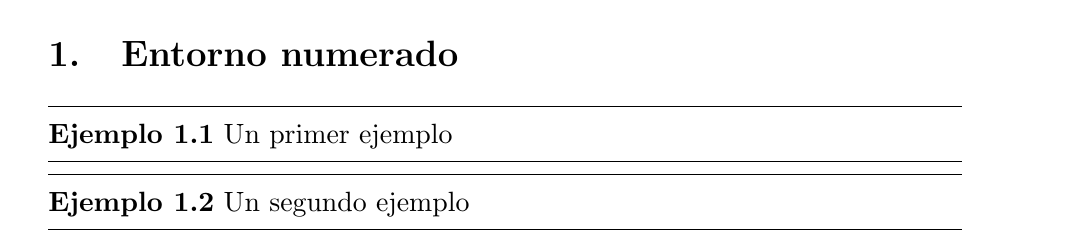
\includegraphics[width=\textwidth]{docs/Figuras/entornoNum.png}
\caption{Entornos numerados}
\end{figure}

\subsection{Entornos trucados}

Al igual que modificábamos comandos existentes con
\lstinline!\renewcommand!, podemos cambiar entornos con
\lstinline!\renewenvironment!:

\begin{lstlisting}[language={[latex]tex}]
\renewenvironment{ENTORNO}[ARGUMENTOS]{ANTES}{DESPUÉS}
\end{lstlisting}

Lo que tenemos que tener en cuenta aquí es la implementación original
del entorno que vamos a cambiar. A mí me ayuda pensar en un entorno como
dos comandos, uno que da inicio al formato concreto y otro que lo
finaliza. Es decir, esto:

\begin{lstlisting}[language={[latex]tex}]
\begin{equation}
  a^2 x + b x + c = 0
\end{equation}
\end{lstlisting}

es equivalente a:

\begin{lstlisting}[language={[latex]tex}]
\equation
  a^2 x + b x + c = 0
\endequation
\end{lstlisting}

De esta manera me resulta más sencillo saber qué hay que escribir en los
argumentos \lstinline!ANTES! y \lstinline!DESPUÉS! de los que hablaba.

Para terminar con los entornos os dejo con un ejemplo complejo que monté
juntando piezas de aquí y de allí para que las citas aparecieran en gris
oscuro con una barrita gris clara a la izquierda. Es complicadillo y yo
misma no sé si lo entiendo muy bien, pero es para que veáis un caso
real:

\begin{lstlisting}[language={[latex]tex}]
\usepackage{framed}

% Redefinir leftbar
\renewenvironment{leftbar}[1][\hsize]
  {\color{gray}
    \def\FrameCommand
    {{\color{lightgray}\vrule width 3pt}}
    \MakeFramed{\hsize#1\advance\hsize-\width\FrameRestore}
  }
  {\endMakeFramed}
  
% Guardar entorno quote, lo forman dos comandos
\let\oldquote=\quote
\let\oldendquote=\endquote

% Barra vertical a la izquierda de la cita
\renewenvironment{quote}
  {\vspace{10pt}\leftbar\vspace*{-6pt}\oldquote}
  {\oldendquote\endleftbar\vspace{10pt}}
\end{lstlisting}

En fin, creo que la única manera de aprender a modificar entornos es
modificar entornos así que no queda más remedio que practicar.

\section{Una nota sobre TeX}

En el principio de los tiempos dijimos que LaTeX es un conjunto de
macros escritos en TeX (o Plain TeX) ¿recordáis? Esto provoca que LaTeX
tenga algunas limitaciones a la hora de definir cosas, limitaciones que
TeX, al ser de más bajo nivel, no tiene.

El comando \lstinline!\let! que hemos usado para guardar la definición
original de un comando que íbamos a modificar pertenece a TeX. También
\lstinline!\def! que
aparece en ejemplo de las citas personalizadas es parte de TeX y sirve
para definir comandos nuevos, al igual que
\lstinline!\newcommand!\footnote{Se pueden declarar comandos nuevos
  dentro de entornos de manera similar a declararlos de manera
  independiente.
  \href{https://en.wikibooks.org/wiki/LaTeX/Macros\#Declare_commands_within_new_environment}{Aquí}
  tenéis más información.}. Os hablo de ellos porque los veréis a menudo
cuando busquéis ejemplos por ahí.

\section{En definitiva, ¿qué hay que
saber?}

Diría que lo más importante es saber la diferencia entre \emph{definir}
(\lstinline!\new!) y \emph{pisar} (\lstinline!\renew!) un comando o
entorno existente y cuándo hay que hacer lo uno o lo otro. Tampoco está
de más recordar que escribimos tanto las definiciones como las
modificaciones en el preámbulo. Igualmente, nos viene bien saber de la
existencia de comandos de TeX como \lstinline!\let! y \lstinline!\def!
que nos hacen la vida más fácil.

Para acabar, os dejo mi proceso para crear macros:

\begin{enumerate}
\def\labelenumi{\arabic{enumi}.}
\item
  Escribo mi combinación de comandos en el cuerpo del documento y
  verifico que funciona.
\item
  Escribo cómo quiero que sea mi comando o entorno final y lo comparo
  con mi combinación de comandos.
\item
  Traslado la combinación al preámbulo y le doy forma según la sintaxis
  correspondiente.
\item
  Extraigo los argumentos y pienso si puedo darle un valor por defecto a
  alguno de ellos.
\item
  Pruebo si funciona.
\end{enumerate}

Lo dicho, a escribir macros se aprende escribiendo macros. ¡Dadle duro!

\section{Referencias}\label{referencias}

\href{http://alvinalexander.com/blog/post/latex/create-your-own-commands-in-latex-using-newcommand}{\emph{LaTeX
example: How to create your own commands with \lstinline!newcommand!}}

\href{https://en.wikibooks.org/wiki/LaTeX/Macros}{\emph{LaTeX/Macros} en
Wikibooks}

\href{http://www.shawnlankton.com/2008/01/newcommand-with-argument-in-latex/}{\emph{\\newcommand
with arguments in LaTeX}}

\href{https://tex.stackexchange.com/questions/35564/plain-tex-vs-latex-macros}{\emph{Plain
TeX vs.~LaTeX Macros} en TeXExchange}

\href{https://en.wikibooks.org/wiki/LaTeX/Plain_TeX}{\emph{LaTeX/Plain
TeX} en Wikibooks}

\href{https://tex.stackexchange.com/questions/26742/list-of-higher-level-latex-commands-corresponding-to-tex-commands/26922\#26922}{\emph{List
of higher-level LaTeX commands corresponding to TeX commands} en
TeXExchange}

\href{https://tex.stackexchange.com/questions/655/what-is-the-difference-between-def-and-newcommand}{\emph{What
is the difference between \\def and \\newcommand?} en TeXExchange}


\chapter{Abramos la caja de herramientas}
Ya sabemos usar LaTeX, crear documentos complejos, presentaciones y
hasta macros propias. Este capítulo es un poco diferente a los
anteriores ya que en lugar de averiguar cómo se hacen las cosas en
LaTeX, vamos a hablar de herramientas externas y trucos que nos pueden
ayudar a la hora de crear nuestro documento.

Veremos algunos paquetes que simplifican el proceso de probar el
formato, cómo crear una plantilla o un registro de cambios y algunas
herramientas que no pertenecen a LaTeX propiamente dicho pero que son
interesantes.

\section{Fase de pruebas}

Vamos a ver dos partes del proceso de testar nuestro precioso formato:
crear un borrador y generar un documento de prueba en el que podemos
cambiar el formato sin necesidad de tener contenido.

\subsection{Un borrador}

Podemos crear un borrador del documento gracias al argumento opcional
\lstinline!draft! de \lstinline!\documentclass!. Tiene dos ventajas:

\begin{itemize}
\item
  \textbf{Se reduce el tiempo de compilación} ya que no se pinta todo el
  contenido. Por ejemplo, se sustituyen las imágenes por cajas del mismo
  tamaño que contienen el nombre de la imagen.
\item
  \textbf{Permite ver más fácilmente errores} como las
  \href{http://www.tex.ac.uk/FAQ-overfull.html}{\emph{overfull
  boxes}}\footnote{Las \emph{overfull boxes} ocurren a menudo porque
    LaTeX no sabe cómo partir una palabra (pasa mucho con las
    direcciones de correo electrónico y las URLs) y haga lo que haga el
    pobre acaba invadiendo el margen, ahí tenemos que
    \href{https://en.wikipedia.org/wiki/Hyphenation_algorithm}{entrar
    nosotros}}, lugares en los que el texto invade el margen, que marca
  con una barra.
\end{itemize}

Muchos paquetes tienen esta opción, cada cual con
\href{https://tex.stackexchange.com/questions/49277/what-does-the-draft-mode-change}{sus
características concretas}. Si establecemos \lstinline!draft! como
opción de la clase afecta a todos ellos, si queremos que solo afecte a
alguno, podemos darla como opción del paquete.

\subsection{Texto e imágenes de
prueba}

Existen un par de paquetes que nos rellenan las páginas de texto sin
sentido para que nos resulte más fácil ver el efecto de algún paquete u
opción. El más sencillito es
\href{https://www.ctan.org/pkg/lipsum}{\lstinline!lipsum!}, la
implementación para LaTeX del típico
\href{https://es.wikipedia.org/wiki/Lorem_ipsum}{\emph{Lorem Ipsum}}. No
puede ser más fácil de usar:

\begin{lstlisting}[language={[latex]tex}]
\documentclass[draft]{article}
\usepackage{lipsum}
\begin{document}
  \lipsum % Texto Lorem Ipsum completo
  \lipsum[17] % El párrafo 17 será texto sin sentido
\end{document}
\end{lstlisting}

Otra opción un poco más potente es \lstinline!blindtext!, que tiene
varias ventajas respecto a \lstinline!lipsum!:

\begin{itemize}
\item
  Depende del idioma así que se puede ver qué tal va la silabación.
  Ahora mismo los idiomas disponibles son inglés, francés, alemán, latín
  y catalán.
\item
  A diferencia del paquete \lstinline!lipsum!, que solo nos crea texto,
  tenemos la posibilidad de generar listas, ecuaciones y hasta un
  documento completo si se lo pedimos.
\item
  Podemos crear texto formado por
  \href{https://es.wikipedia.org/wiki/Pangrama}{pangramas}, frases que
  contienen todas las letras del abecedario de un idioma concreto,
  interesante para probar tipografías. También podemos usar trozos de la
  Biblia, cosa que me parece absolutamente genial aunque utilidad
  práctica le veo menos.
\end{itemize}

Veamos ahora cómo se usa, que es un poco más complejo que
\lstinline!lipsum!. Para crear texto tenemos dos comandos:

\begin{itemize}
\item
  \lstinline!\blindtext! crea un trozo de texto corto. Opcionalmente le
  podemos dar el número de veces que queremos que repita el texto con
  \lstinline!\blindtext[REPETICIONES]!.
\item
  \lstinline!\Blindtext! crea un trozo de texto largo. Puede tomar como
  opciones el número de párrafos y el de repeticiones con
  \lstinline!\Blindtext[PARRÁFOS][REPETICIONES]!
\end{itemize}

Podemos fabricar un documento completo, largo o corto, con y sin
ecuaciones:

\begin{itemize}
\item
  \lstinline!\blindocument! crea un documento corto, si delante
  activamos las matemáticas con \lstinline!\blindmathtrue! tendrá
  también ecuaciones. El documento tendrá títulos de sección de todos
  los niveles y varios tipos de listas.
\item
  \lstinline!\Blindocument! crea un documento largo, funciona
  exactamente igual que el anterior.
\item
  \lstinline!\blindmathpaper! crea un documento con ecuaciones.
\end{itemize}

Hay otras opciones para crear listas y así, en el
\href{http://osl.ugr.es/CTAN/macros/latex/contrib/blindtext/blindtext.pdf}{manual}
lo tenéis bien explicado.

En cuanto a las \textbf{imágenes}, el paquete
\href{http://www.ctan.org/pkg/mwe}{\lstinline!mwe!} (\emph{Minimal
Working Example}) nos proporciona diversas imágenes de prueba\footnote{Viven
  en \lstinline!/usr/share/texlive/texmf-dist/tex/latex/mwe/! si las
  queréis mirar.} de diferentes proporciones y formatos. Este paquete
también nos carga \lstinline!graphicx! y si están instalados,
\lstinline!lipsum! y \lstinline!blindtext!. No hace falta que carguemos
el paquete para usar estas imágenes, las instala de tal manera que al
compilar se pueda acceder a ellas.

Para usarlas simplemente las llamamos por su nombre:

\begin{lstlisting}[language={[latex]tex}]
\includegraphics{example-image-a}
\end{lstlisting}

\section{Una plantilla}

Cuando ya tengamos nuestro formato perfectamente definido, si vamos a
usarlo a menudo podemos crear una plantilla a partir del documento.
Todos los IDEs que yo conozco permiten exportar una plantilla a partir
del documento actual, más adelante podremos importarla y tendremos una
base desde la que trabajar.

Otra opción es crear nuestra propio paquete (\emph{sty}) o clase
(\emph{cls}). Crearemos un paquete si nuestras macros valen para
diferentes clases, y si, en cambio,estamos definiendo un tipo de
documento, crearemos una clase. Tanto las clases como los paquetes
consisten en lo que escribimos en el preámbulo de nuestros documentos
formateado de otra manera.

Os pongo como ejemplo un paquete muy poco ortodoxo que nos carga los
paquetes de idioma para cuando queremos escribir en español. Consistiría
en el archivo \lstinline!español.sty! con el siguiente contenido:

\begin{lstlisting}[language={[latex]tex}]
% Versión de LaTeX usada
\NeedsTeXFormat{LaTeX2e}[1994/06/01]

% Nombre del paquete creado
\ProvidesPackage{español}

% Paquetes usados
\RequirePackage[utf8]{inputenc}
\RequirePackage[spanish]{babel}
\RequirePackage[T1]{fontenc}
\RequirePackage{lmodern}
\end{lstlisting}

Como veis, usamos \lstinline!\RequirePackage! en lugar de
\lstinline!\usepackage!, pero se parece bastante a un preámbulo de toda
la vida. Guardamos nuestro paquete en un lugar accesible y lo llamamos
como a cualquier otro con \lstinline!\usepackage{español}!.

Hay más información sobre la creación de clases y paquetes en las
referencias.

\section{Cambios y versiones}

Que manejemos texto plano tiene una gran ventaja: podemos fácilmente
incluir software de control de versiones en nuestro flujo de trabajo.
Además de las ventajas que ya tiene el control de versiones de por sí,
nos permite incluir información sobre las versiones y los cambios en el
propio documento

Tenemos, además, un montón de paquetes para añadir información sobre los
cambios al documento. Algunos incluyen al pie o en una marca de agua la
versión actual, como
\href{http://ctan.org/pkg/gitinfo2}{\lstinline!gitinfo2!}, con otros
como
\href{http://www.ctan.org/tex-archive/macros/latex/contrib/vhistory}{\lstinline!vhistory!}
registramos el historial de cambios en una tabla de manera manual
mediante el comando \lstinline!\vhEntry!:

\begin{lstlisting}[language={[latex]tex}]
\vhEntry{VERSIÓN}{FECHA}{AUTOR}{CAMBIOS}
\end{lstlisting}

Después, podemos hacer referencia a esta información en el cuerpo del
documento, ya sea el número de versión o la lista de autores.
\href{http://osl.ugr.es/CTAN/macros/latex/contrib/vhistory/doc/vh_sets_en.pdf}{Aquí}
tenéis el manual del paquete si queréis echarle un ojo.

Es fácil crear \textbf{registro de cambios} casero si usamos
\lstinline!git!. Una manera es etiquetar los puntos más interesantes,
exportar una tabla con la información deseada e incluirla en el
documento mediante el comando \lstinline!\input{}!.

Para etiquetar podemos usar una etiqueta \emph{anotada} o \emph{ligera},
con la primera podemos añadirle un mensaje a la etiqueta, la ligera
simplemente marca el \emph{commit} anterior. Yo voy a usar etiquetas
ligeras como ejemplo. Procedamos:

\begin{lstlisting}[language=bash]
git tag NOMBRE
\end{lstlisting}

Luego, para exportar en formato LaTeX la información de cada etiqueta
que hemos creado usamos algo de este estilo, dependiendo de qué queramos
conseguir:

\begin{lstlisting}[language=bash]
git for-each-ref --format="%(refname:short) & %(authordate:short) & %(subject) \\\\" refs/tags > log.tex
\end{lstlisting}

Como hemos formateado la información como si fuera el contenido de una
tabla (¡mirad los separadores de columna y el salto de línea!) , lo
incluimos dentro de un entorno \lstinline!tabular! en el que escribimos
los encabezados:

\begin{lstlisting}[language={[latex]tex}]
\begin{tabular}{l l l}
  \textbf{Versión} & \textbf{Fecha} & \textbf{Descripción} \\
  & & \\
  \input{log.tex} % incluir datos
\end{tabular}
\end{lstlisting}

Por supuesto, podríamos crear una macro, formatear la información de
cualquier otro modo o incluso fusionarlo con el paquete
\lstinline!vhistory!, simplemente os enseño mi sistema, a partir de ahí
cada que haga uso de su libre albedrío.

Para automatizar esto hay varias maneras, una de ellas es escribir un
\emph{hook} de \lstinline!git!, otra es incluir la línea anterior en el
Makefile, si lo estamos usando, y la más simple es modificar la orden de
compilación que ejecuta nuestro IDE.

Cambiando ligeramente de tema, una manera interesante de \textbf{mostrar
los cambios} entre dos versiones de un documento es
\href{https://www.ctan.org/pkg/latexdiff?lang=en}{\lstinline!latexdiff!},
un \emph{script} de Perl que compara dos archivos de LaTeX y genera un
tercer archivo destacando los cambios.

Una vez instalados Perl y \lstinline!latexdiff!, si no los teníamos ya,
no hay más que escribir lo siguiente en la terminal\footnote{Si estáis
  en Windows y
  \href{http://techshangrila.blogspot.com.es/2013/10/installing-latexdiff-of-windows.html}{después
  de instalar Perl} no os funciona, probad \lstinline!latexdiff-so!, la
  versión \emph{standalone}. Hablé de ello un poco más en detalle
  \href{https://ondahostil.wordpress.com/2016/09/16/lo-que-he-aprendido-latexdiff-vuelve-a-la-carga/}{aquí}.}:

\begin{lstlisting}[language=bash]
latexdiff viejo.tex nuevo.tex > dif.tex
\end{lstlisting}

Si compilamos \lstinline!dif.tex! conseguiremos algo así:

\begin{figure}[htbp]
\centering
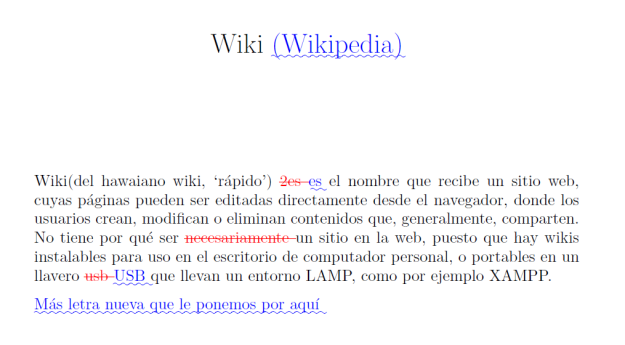
\includegraphics[width=\textwidth]{docs/Figuras/diff.png}
\caption{Marcando las diferencias}
\end{figure}

Tacha en rojo lo que hemos borrado y destaca en azul lo que hemos
añadido. Me parece especialmente útil para cuando estamos colaborando,
se ve de un vistazo cómo quedan los cambios.

Por cierto, si no queréis instalar nada también hay una
\href{https://3142.nl/latex-diff/}{versión online} en la que pegamos el
contenido de los archivos a comparar y nos aparece el archivo de
diferencias que podemos a su vez copiar y compilar.

\section{Exportar a LaTeX}

Este último apartado sobre las herramientas trata de exportar contenido
que tenemos en otros formatos a LaTeX. De esta manera conseguimos dos
cosas:

\begin{itemize}
\item
  Incluir con facilidad contenido creado en otros programas en LaTeX.
\item
  Ayudarnos a crear elementos que resultan complejos de llevar a cabo en
  LaTeX, como podrían ser las tablas y las portadas.
\end{itemize}

En el caso de las tablas se entrelazan ambas problemáticas, cuesta
escribir tablas en LaTeX y, además, muchas veces tenemos esas tablas en
otros formatos. Si nuestro problema es el primero, tenemos
\href{http://www.tablesgenerator.com/}{\emph{editores online}} con los
que crear la tabla de manera visual y exportarla a continuación. Si nos
pasan un poco de las dos cosas tenemos varias herramientas, la que más
he usado ha sido
\href{http://www.ctan.org/tex-archive/support/excel2latex/}{\emph{Excel2Latex}},
un \emph{plugin} para Excel que nos permite seleccionar y exportar una
tabla concreta en formato LaTeX, la verdad es que funciona bastante
bien. También hay una versión para OpenOffice,
\href{http://calc2latex.sourceforge.net/}{\emph{Calc2LaTeX}}, pero es
viejecita y no sé qué tal funciona, y tenemos
\href{https://github.com/TheChymera/matrix2latex}{\emph{Matrix2LaTeX}}
para Python y Matlab que no he usado.

Una herramienta similar es
\href{https://extensions.libreoffice.org/extensions/writer2latex-1}{\emph{Writer2LaTeX}}
que sirve para exportar de Libre Office Writer a LaTeX, no es la panacea
pero nos puede ayudar cuando tenemos que seguir cierta plantilla y solo
nos proporcionan un \emph{doc}, ¿os suena esto?

Sin duda el programa definitivo para las labores de conversión es
\href{http://pandoc.org/}{\emph{Pandoc}}, del que ya hemos hablado y que
trataremos largo y tendido dentro de poco. Con una terminal y una orden
muy sencilla transforma casi cualquier formato de texto a casi cualquier
otro:

\begin{lstlisting}[language=bash]
pandoc OPCIONES INPUT -o OUTPUT
\end{lstlisting}

\section{Resumen}

En este capítulo he mencionado diferentes herramientas útiles sin entrar
demasiado en detalle para que vosotros mismos investiguéis las que mejor
se adapten a vuestras necesidades. Hemos hablado de borradores, texto e
imágenes de prueba, plantillas, clases y paquetes, control de versiones
y sobre cómo exportar el contenido creado en otros programas a LaTeX.
Evidentemente, hay muchas más herramientas relacionadas con LaTeX ahí
fuera, estas son las que me han servido a mí en mi larga relación con
este lenguaje de marcado tan simpático.

\section{Referencias}

\href{https://tex.stackexchange.com/questions/49277/what-does-the-draft-mode-change}{\emph{What
does the draft mode change?} en TeXExchange}

\href{http://tug.ctan.org/info/dickimaw/dickimaw-minexample.pdf}{\emph{Creating
a LaTeX Minimal Example} (pdf)}

\href{https://www.ctan.org/pkg/lipsum}{El paquete \lstinline!lipsum!}

\href{https://www.ctan.org/pkg/blindtext}{El paquete
\lstinline!blindtext!}

\href{http://tex.stackexchange.com/questions/231738/example-images-in-latex\#231741}{\emph{Example
images in LaTeX?} en TexExchange}

\href{https://tex.stackexchange.com/questions/278817/creating-a-default-preamble}{\emph{Creating
a default preamble} en TeXExchange}

\href{https://docs.kde.org/stable4/en/extragear-office/kile/kile.pdf}{Manual
de Kile (pdf)}

\href{http://texstudio.sourceforge.net/manual/current/usermanual_en.html\#SECTION12aa}{Manual
de TexStudio}

\href{https://en.wikibooks.org/wiki/LaTeX/Creating_Packages}{\emph{LaTeX/Creating
Packages} en Wikibooks}

\href{http://www.latex-project.org/help/documentation/clsguide.pdf}{\emph{LaTeX
2$\varepsilon$ for class and package writers}}

\href{https://tex.stackexchange.com/questions/6560/best-practice-for-maintaining-change-history-in-tex}{\emph{Best
practice for maintaining change history in tex} en TeXExchange}

\href{https://robjhyndman.com/hyndsight/tracking-changes-in-latex-files/}{\emph{Tracking
changes in LaTeX files}}

\href{https://ondahostil.wordpress.com/2017/04/24/lo-que-he-aprendido-registro-de-cambios-en-un-documento-latex-con-git/}{\emph{Registro
de cambios en un documento LaTeX con git}}

\href{https://tex.stackexchange.com/questions/161/latex-packages-for-use-with-revision-control}{\emph{LaTeX
packages for use with revision control}}

\href{http://techshangrila.blogspot.com.es/2013/10/installing-latexdiff-of-windows.html}{\emph{Highlighting
the different between Latex Documents in Windows 7 using Latexdiff}}

\href{https://en.wikibooks.org/wiki/LaTeX/Collaborative_Writing_of_LaTeX_Documents}{\emph{LaTeX/Collaborative
Writing of LaTeX Documents} en Wikibooks}

\href{https://support.rstudio.com/hc/en-us/articles/200532257-Customizing-LaTeX-Options}{\emph{When
and why should I use \% !TEX TS-program and \% !TEX encoding?} en
TeXExchange}

\href{https://latexforhumans.wordpress.com/tag/calc2latex/}{\emph{Converting
a spreadsheet to LaTeX}}


\appendix
\chapter{Una nota sobre los archivos auxiliares}
Os habréis fijado como yo en que cuando compilamos LaTeX desde un IDE se
generan miles y miles de archivos auxiliares al darle a que genere el
documento. Vamos a ver si conseguimos clarificar un poco que para qué
sirven algunos de ellos.

Aquí tenemos un lista de los archivos auxiliares más típicos, lo mejor
de todo es que todos ellos son texto plano así que podemos abrirlos y
mirar qué contienen:

\begin{itemize}
\item
  \lstinline!aux!: sirve para gestionar las referencias cruzadas
  (\lstinline!\ref!) y las citas bibliográficas (\lstinline!\cite!),
  entre otras cosas. En general, guarda la información que ha de pasarse
  de un proceso de compilación a otro.
\item
  \lstinline!log!: aquí se guarda la información sobre el proceso de
  compilación, las advertencias, los errores, los paquetes utilizados
  con su respectiva versión y tal. Es especialmente útil si nos falla al
  crear el documento y no sabemos por qué.
\item
  \lstinline!synctex!: sincroniza nuestro código fuente con el documento
  de salida en el IDE, es decir, al movernos por el código fuente vemos
  al lado la parte correspondiente del \emph{pdf}. Podemos borrarlo
  alegremente, simplemente se creará otro.
\item
  \lstinline!toc!, \lstinline!lof!, \lstinline!lot! \ldots{} : sirven
  para crear el índice, la lista de figuras, la lista de tablas \ldots{}
\item
  \lstinline!out!: lo genera \lstinline!hyperref! y vale para crear los
  enlaces que nos llevan de un lado a otro en el \emph{pdf}.
\item
  \lstinline!bbl!: es el archivo de bibliografía creado por BibTeX.
\item
  \emph{Otros}: otros paquetes crean archivos auxiliares para gestionar
  sus cosas, por ejemplo, el paquete
  \href{http://ctan.org/pkg/listofsymbols}{\lstinline!listofsymbols!}
  crea un \lstinline!sub! y un \lstinline!sym! para gestionar la lista
  de subíndices y de símbolos respectivamente. Otro ejemplo son los
  archivos \lstinline!idx! que sirven para hacer el índice por palabras
  con
  \href{https://en.wikibooks.org/wiki/LaTeX/Indexing}{\lstinline!makeindex!}.
\end{itemize}

Para el caso de Beamer se crean además estos otros:

\begin{itemize}
\item
  \lstinline!snm!: ayuda en el proceso de insertar imágenes en el tipo
  \lstinline!article!
\item
  \lstinline!nav!: sirve para crear la barra de navegación en la
  presentación
\end{itemize}

Todos estos archivos aparecen porque cuando nosotros le damos al
botoncillo para que nos cree el documento por dentro en realidad se
invocan un montón de procesos. Tomando como ejemplo un caso en el que
usemos \lstinline!pdflatex! y tengamos referencias se haría algo así:

\begin{lstlisting}[language=bash]
pdflatex fuente.tex  # primera compilación
bibtex fuente.aux    # la bibliografía
pdflatex fuente.tex  # para referencias 
pdflatex fuente.tex  # para referencias 
\end{lstlisting}

Como veis, necesitamos compilar tres veces para tener las referencias
correctamente. A este proceso se le pueden añadir otros pasos como
\lstinline!makeindex!, para el índice por palabras, o
\lstinline!makeglossaries!, para crear el glosario. Es por esta ristra
de procesos que nosotros no vemos que se escriben todos los archivos
auxiliares.

Os preguntaréis: \emph{¿estas mierdas para qué las va dejando por ahí?
¿no las puede crear y luego borrarlas?} Podría hacerlo, sí, Pandoc lo
hace de hecho, crea una carpeta temporal con las basuras y luego la
borra. Esto es como todo en la vida, tiene sus ventajas y sus
inconvenientes. Tener esos archivos auxiliares nos permite hurgar y
trucar cosas y es útil para ver dónde falla al compilar. Pero si no os
gusta que os deje cosas por ahí tenéis varias opciones:

\begin{itemize}
\item
  Si usáis un IDE tipo Kile, tendréis un botón para eliminar los
  archivos auxiliares.
\item
  Si el documento no tiene referencias cruzadas, ni citas
  bibliográficas, ni ninguna cosa que necesite archivos auxiliares
  podemos usar \lstinline!\nofiles! en el preámbulo y solo nos creará el
  \lstinline!pdf!y el \lstinline!log!. También se creará el
  \lstinline!synctex! si compilamos desde un IDE. Tampoco nos ahorramos
  mucha cosas como veis.
\item
  Añadir \lstinline!--aux-directory=CARPETA! a la orden de compilar. Así
  meterá todos los archivos auxiliares en la carpeta que le hemos dicho
  y buscará también ahí cuando los necesite. Lo podemos cambiar
  fácilmente en el IDE donde aparecen las órdenes. Esta es la opción que
  yo suelo usar (ahora que la he descubierto).
\item
  Compilar con la opción \lstinline!--jobname=CARPETA/OUTPUT INPUT.tex!,
  así guardará el \emph{pdf} y los archivos auxiliares en la carpeta que
  nosotros queramos\footnote{¡Gracias Shevek por hablarme de esta
    opción!}.
\item
  Usar \emph{Pandoc}. Esto nos hace cambiar nuestra forma de trabajar
  radicalmente, pero no nos quedan sobras por ahí.
\end{itemize}

\section{Referencias}

\href{http://www.dickimaw-books.com/latex/novices/html/auxiliary.html}{\emph{Auxiliary
Files} en Dickimaw Books}

\href{http://tex.stackexchange.com/questions/11123/prevent-pdflatex-from-writing-a-bunch-of-files}{\emph{Prevent
pdflatex from writing a bunch of files} en TeXExchange}

\href{http://stackoverflow.com/questions/3745908/i-dont-want-the-aux-log-and-synctex-gz-files-when-using-pdflatex}{\emph{I
don't want the .aux, .log and .synctex.gz files when using pdflatex} en
StackOverflow}

\href{http://latex-mk.sourceforge.net/}{\lstinline!latex-mk!}


\chapter{Hablemos de paquetes}
En todo el curso no he hablado de instalación pero me parecía necesaria
una pequeña nota sobre los paquetes, especialmente para el caso de
GNU/Linux, ya que la distribución de LaTeX para Windows, MikTeX, instala
los paquetes necesarios de manera automática.

El caso de TeXLive es diferente porque hay dos maneras\footnote{También
  se pueden descargar los paquetes de CTAN y descomprimirlos en la
  carpeta correcta de nuestro LaTeX tal y como cuentan
  \href{https://en.wikibooks.org/wiki/LaTeX/Installing_Extra_Packages}{aquí},
  nunca lo he hecho y me parece un poco lioso.} de instalarlo en
GNU/Linux:

\begin{itemize}
\item
  \textbf{Desde los repositorios de nuestra distro}, cuando queramos
  instalar paquetes usaremos también los repositorios.
\item
  \textbf{Descargándolo
  \href{https://www.tug.org/texlive/doc/texlive-en/texlive-en.html\#installation}{por
  ahí}}, lo que suelen llamar \emph{TeXLive nativo}. En este caso habrá
  que usar el gestor de paquetes de TeXLive.
\end{itemize}

\section{Descargar paquetes desde los repositorios}

Los paquetes de TeXLive viven en paquetes de los repositorios (de
Debian, en mi caso\footnote{Creo que funciona de la misma manera en
  todas las distros, tenéis información específica
  \href{http://tug.org/texlive/distro.html}{aquí}.}) pero \emph{no
directamente con su nombre}. Me explico con un ejemplo: el soporte de
idioma.

Sabemos que para que LaTeX nos haga bien la silabación y que use las
palabras claves (\emph{Capítulo}, \emph{Sección}, \ldots{}) en el idioma
correspondiente necesitamos el paquete \lstinline!babel! con el idioma
como opción:

\begin{lstlisting}[language={[latex]tex}]
\usepackage[spanish]{babel}
\end{lstlisting}

Si hemos instalado la versión sencilla de TeXLive y añadimos esa línea a
nuestro \emph{tex} nos dará error al compilar porque nos falta el
paquete de español. Para buscarlo hacemos\footnote{Para ver cuál es el
  comando para buscar paquetes equivalente a
  \lstinline!apt-cache search! en otras distros podéis usar
  \href{https://colaboratorio.net/gestor-paquetes.html}{esta tabla} de
  los \emph{compis} de \href{https://colaboratorio.net/}{Colaboratorio}.}:

\begin{lstlisting}[language=bash]
apt-cache search texlive spanish
\end{lstlisting}

Veremos lo siguiente:

\begin{lstlisting}[language=bash]
texlive-latex-extra - TeX Live: LaTeX additional packages
texlive-doc-es - TeX Live: transitional dummy package
texlive-lang-spanish - TeX Live: Spanish
\end{lstlisting}

Esto nos da una pista de donde vive el paquete: en el grupo de paquetes
adicionales (\lstinline!texlive-latex-extra!) o en uno específico de
idioma (\lstinline!texlive-lang-spanish!). Ahora podemos instalar el que
prefiramos.

Resumiendo: \emph{cada vez que necesitemos un paquete de TeXLive debemos
buscar el paquete de los repositorios que lo contiene}. Este sistema es
cómodo pero tiene el problema de que los paquetes suelen ser ancianos,
de ahí la utilidad del segundo método.

\section{El gestor de paquetes de
TeXLive}

También se pueden instalar los paquetes con \lstinline!tlmgr!, el gestor
de paquetes de TeXLive. Para usar esta opción hay que instalar TeXLive
\href{http://tug.org/texlive/acquire-netinstall.html}{descargándolo de
la red}\footnote{Kile por ejemplo depende de TeXLive así que solo con
  una \emph{instalación nativa} no funcionará. En algunas distros está
  disponible el paquete \lstinline!texlive-dummy! para solucionar este
  problema. En Debian y derivados hay que instalar un
  \href{http://tug.org/texlive/debian.html\#vanilla}{\emph{vanilla
  TeXLive}}.}. Luego instalamos los paquetes escribiendo en la
terminal\footnote{¡También tiene una
  \href{https://darrengoossens.wordpress.com/tag/gui/}{GUI}!}:

\begin{lstlisting}[language=bash]
tlmgr install PAQUETE
\end{lstlisting}

Incluso podemos actualizar todos los paquetes instalados con:

\begin{lstlisting}[language=bash]
tlmgr update --all
\end{lstlisting}

Como siempre, tenemos toda la información sobre este comando en su
\href{https://www.tug.org/texlive/doc/tlmgr.html}{manual} y en este caso
también haciendo:

\begin{lstlisting}[language=bash]
tlmgr --help
\end{lstlisting}

Este sistema tiene la ventaja de que los paquetes que descarguemos
estarán actualizados, aparte de que tendremos acceso a paquetes que
todavía no son parte de los repositorios de nuestra distribución de
GNU/Linux.

\section{Referencias}

\href{http://tex.stackexchange.com/questions/28528/best-way-to-install-packages-for-texlive-in-ubuntu}{\emph{Best
way to install packages for TeXLive in Ubuntu?} en TeXExchange}

\href{https://en.wikibooks.org/wiki/LaTeX/Installing_Extra_Packages}{\emph{LaTeX/Installing
Extra Packages} en Wikibooks}

\href{https://www.tug.org/texlive/quickinstall.html}{\emph{TeX Live -
Quick install}}

\href{http://tex.stackexchange.com/questions/73526/how-to-install-a-language-package-in-texmaker-on-ubuntu-12-04\#73528}{\emph{How
to install a language package in Texmaker on Ubuntu 12.04?} en
TeXExchange}

\href{https://www.tug.org/texlive/pkginstall.html}{\emph{TeX Live
package installation}}

\href{http://tug.org/texlive/distro.html}{\emph{TeX Live and distros}}

\href{http://texblog.org/2011/05/12/updating-latex-tex-live/}{\emph{LaTeX
Installation} en texblog}

\href{https://tex.stackexchange.com/questions/114623/installing-texlive-on-ubuntu-revisited}{\emph{Installing
TeXlive on Ubuntu, revisited} en TeXExchange}

\href{https://wiki.archlinux.org/index.php/TeX_Live}{\emph{TeX Live} en
la wiki de Arch}

\href{https://www.tug.org/texlive/doc/tlmgr.html}{Manual de
\lstinline!tlmgr!}


\chapter{Enlaces de interés}
\section{Información general}

\begin{itemize}
\item
  \href{http://www.dickimaw-books.com/latexresources.html}{\emph{LaTeX
  Resources}} y
  \href{http://www.dickimaw-books.com/latex/index.html}{\emph{LaTeX
  books}} en \href{http://www.dickimaw-books.com/}{\emph{Dickimaw
  Books}} la página donde Nicola L. C. Talbot recopila lo que escribe
  sobre LaTeX y otras cosas.
\item
  \href{http://www.tex.ac.uk/faq/}{\emph{The UK list of TeX Frequently
  Asked Questions}}: una recopilación de dudas de LaTeX que cubre todos
  los aspectos, desde la instalación al formato pasando por los
  paquetes.
\item
  \href{http://www.latex-project.org/}{\emph{The LaTeX project}}:
  información variada sobre LaTeX, noticias y publicaciones.
\item
  \href{http://tug.org/}{\emph{TeX Users Group}}: una web de usuarios de
  LaTeX creada en 1980 con cosas sobre instalación y tipografía.
\end{itemize}

\section{Blogs}

\begin{itemize}
\item
  \href{http://texstudio.de/}{\emph{TeX tips}}: un blog con truquillos
  de LaTeX
\item
  \href{http://www.math.illinois.edu/~ajh/tex/tips.html}{\emph{LaTeX
  Tips}}: más trucos, estos especialmente sobre matemáticas.
\item
  \href{http://www.texdev.net/}{\emph{Some TeX Developments}}: otro
  blog, este más avanzado, suele tratar sobre programar y temas
  complejos.
\item
  \href{http://www.highschoolmathandchess.com/latex/}{\emph{LaTeX} en
  \emph{High School Math and Chess}}: especialmente interesantes la
  lista de paquetes y cuando prueba diferentes tipos de documentos.
\end{itemize}

\section{Cursos}

\begin{itemize}
\item
  \href{http://www.math.tamu.edu/~boas/courses/math696/LaTeX.html}{Curso
  de la Universidad de Texas}
\item
  \href{http://metodos.fam.cie.uva.es/~latex/apuntes/apuntes.html}{Curso
  de la Universidad de Valladolid}
\end{itemize}

\section{Plantillas}

\begin{itemize}
\item
  \href{http://www.latextemplates.com/}{\emph{LaTeX templates}}
\item
  \href{https://www.overleaf.com/}{\emph{Overleaf}}
\end{itemize}

\section{Otros}

\begin{itemize}
\item
  \href{https://tex.stackexchange.com/questions/3/compiling-documents-online}{Una
  lista de herramientas para compilar LaTeX online}
\end{itemize}


% Bibliografía
\backmatter
% \bibliographystyle{plain}
%\bibliography{bib}

\end{document}
